\chapter{Analysis Methods and Corrections} \label{ch:analysis}

Beginning in March of 2012, the LHC began seven months of pp collisions at $\sqrt{s} = \,$ 8 TeV. During the seven months of data taking, the ALICE Experiment was recording data almost 60\% of the time, Figure \ref{fig:RunEffer}, with stable beams.

\begin{figure}[h]
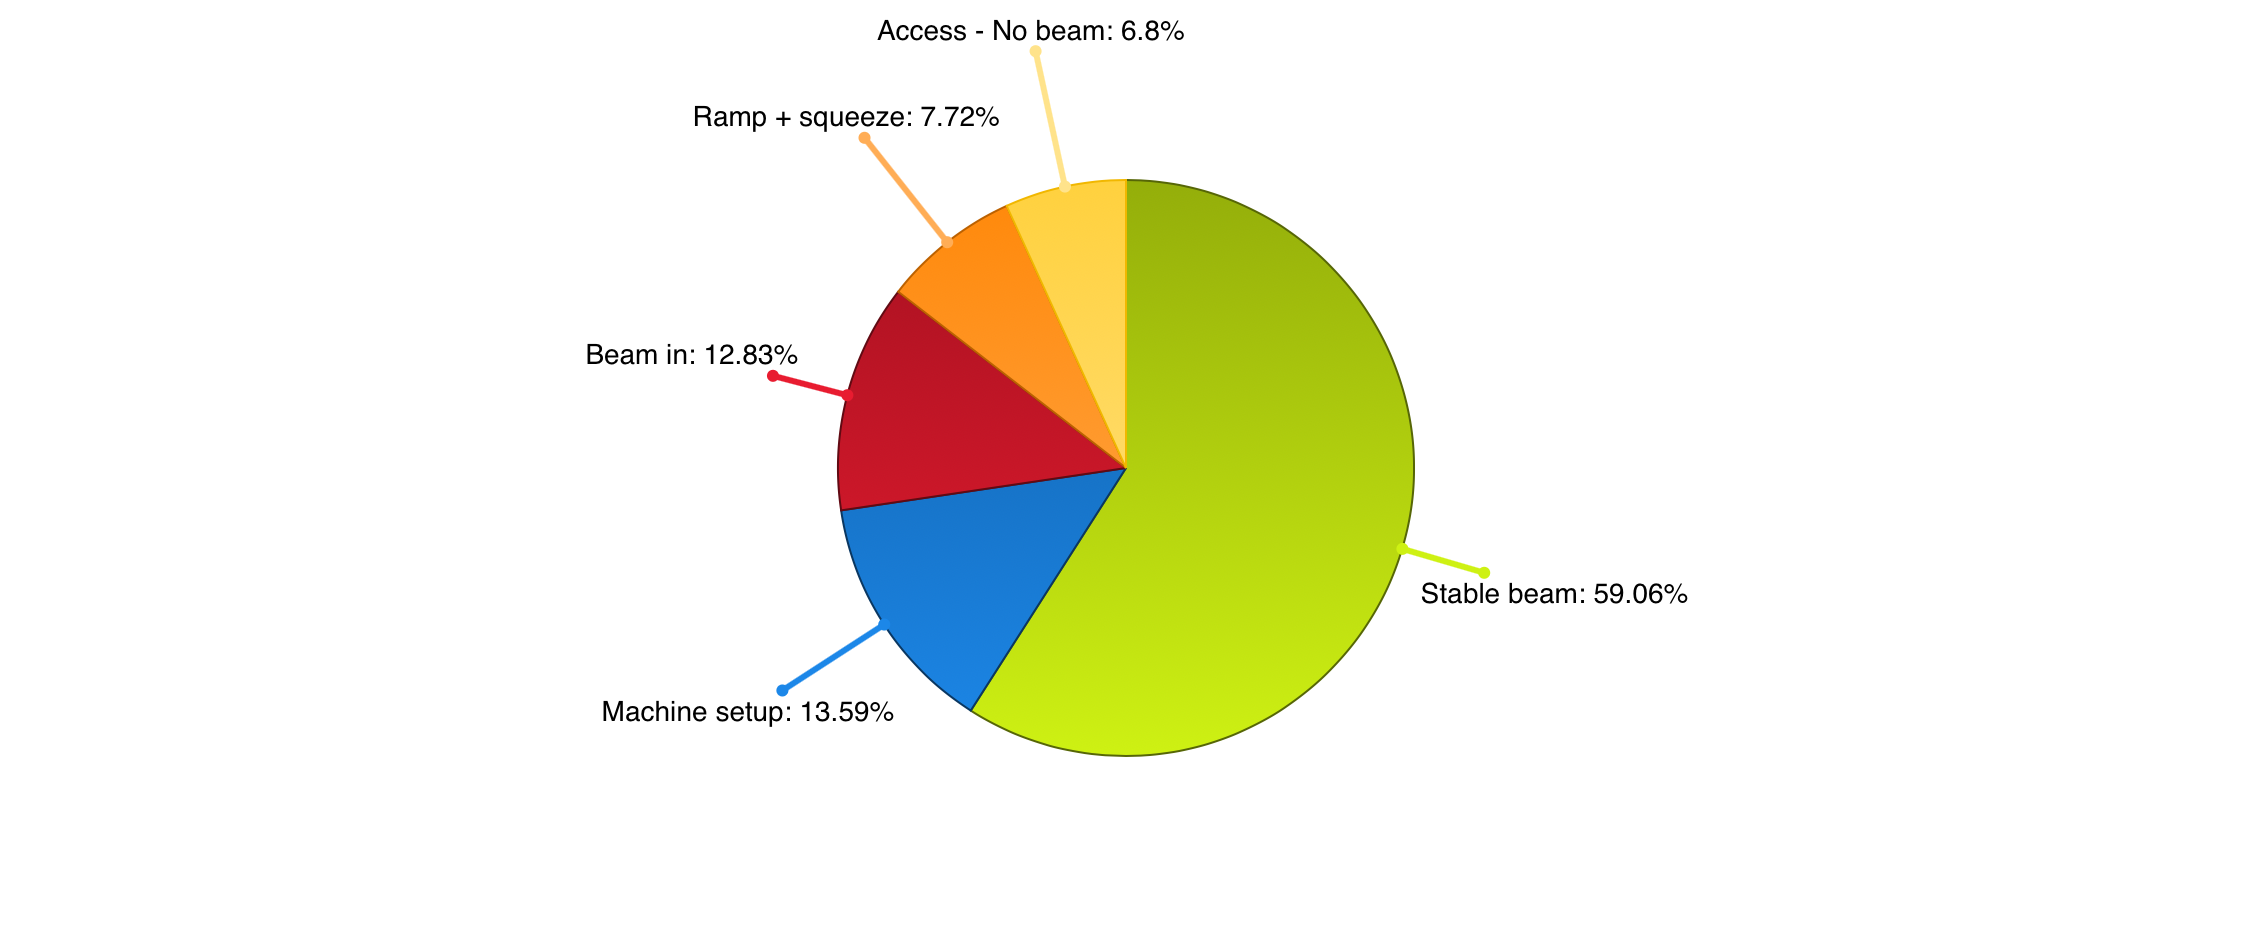
\includegraphics[width=17cm]{8TeVRunefficency}
\centering
\caption{LHC state during the 8 TeV run. }
\label{fig:RunEffer}
\end{figure}


Almost 200 million events were recorded by ALICE that satisfied the Min Bias trigger.  The pp Min Bias trigger is satisfied with at least one hit recorded in the SPD or V0.  The 8 TeV data set also recorded high-$p_{T}$ events using the EMCal triggered data, which in the case of the Gamma trigger was set at 5 GeV.  

This large amount of data offers a unique chance to explore jet cross-sections using high statistics.   In order to measure the jet double differential cross-section, the following formula is used,

\begin{equation}
	\frac{d^{2} \sigma^{jet}}{d\eta \, dp_{T}} = \frac{1}{\epsilon_{reco}} \frac{A_{trigger}}{\epsilon_{trigger}(p_{T})} \times C_{MC} \times \frac{1}{A(p_{T}) } \times \frac{1}{\mathscr{L}_{int}} \times \frac{dN^{2}_{jet}}{dp_{T} \, d\eta}
\label{eq:xsecdef}
\end{equation}

\noindent
where,

\begin{itemize}
  \item $\epsilon_{reco}$ is the efficency for reconstructing the jet in the ALICE detector.
  \item $A_{trigger}$ is the acceptance for EMCal triggered events and $\epsilon_{trigger}(p_{T})$ is the EMCal trigger efficiency.  These factors correct for imperfections in the electronics of the EMCal and the overall factors are equal to one in Min Bias events.
  \item $C_{MC}$ is a correction factor due to detector effects and it allows for comparisons between the ALICE experiment and other experiments or theoretical calculations.  Unfolding is used to determine this factor.
  \item $\mathscr{L}_{int}$ is the integrated luminosity during the period when the data was recorded.
  \item $A(p_{T})$ is the geometrical detector acceptance.
  \item $\frac{dN^{2}_{jet}}{dp_{T} \, d\eta}$ is the inclusive jet momentum spectra.
  
\end{itemize}

\noindent

ALICE is a state-of-the-art experiment with excellent tracking and particle identification capabilities, as discussed in Chapter \ref{ch:alice}.  However, just like any real world experiment, it contains a number of inefficiencies and imperfections.  This means that the data collected during the 8 TeV pp collisions must be examined and any inaccuracies in the data must be removed before any conclusions may be reached.  Data may be compromised at either the event-level, the experiment erroneously recorded something as an event, or at the constituent-level, one of the subdetectors mismeasured a feature of a particle.  The remainder of this chapter focuses on the corrections and quality assurance performed on the 8 TeV data.


\section{Raw Jet Spectra}

This analysis measured inclusive jet results for radii between 0.1 and 0.5.  However, jet results for radii R = 0.2 to R = 0.4 will be presented in the body of this chapter while results from the other jet radii are still being investigated.  Figures \ref{fig:rawjetR02}, \ref{fig:rawjetR03}, and \ref{fig:rawjetR04} show the raw (uncorrected) $p_{T}$ spectra for inclusive jets from both Min Bias and EMCal triggered data.  It is also evident from these figures that the EMCal triggered data greatly extends the kinematic reach of the measured jet spectra, to about 200 GeV/c.  The next sections of this chapter will discuss the QA implemented to the data, trigger scaling, unfolding, and other corrections used in this thesis. 

\begin{figure}[h]
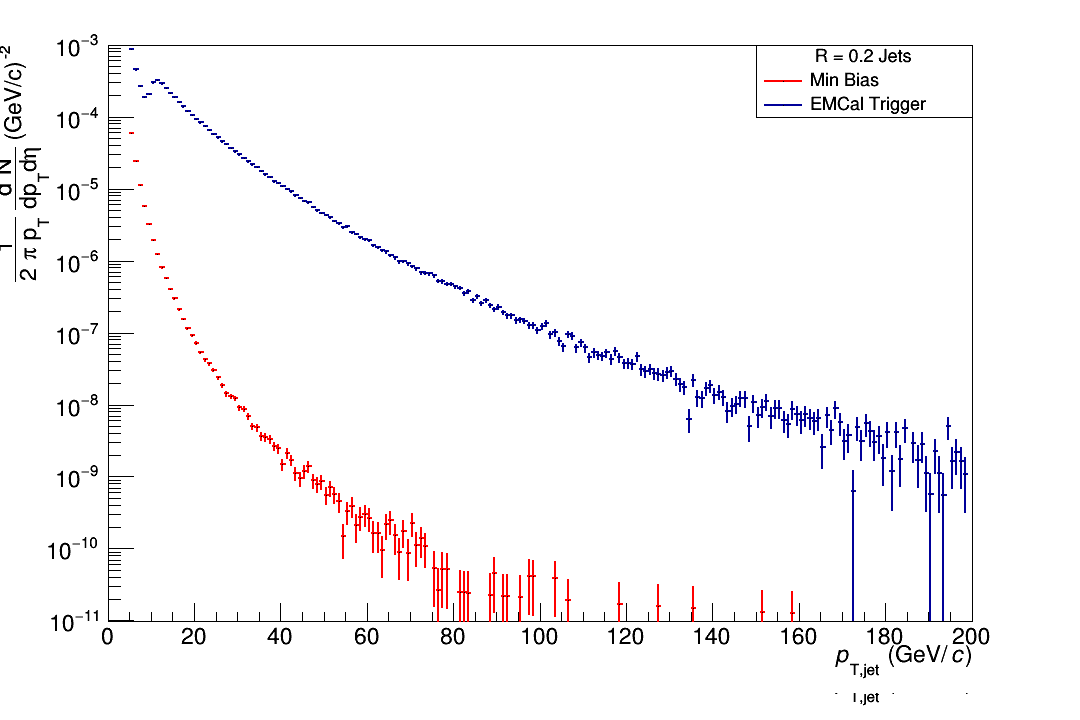
\includegraphics[width=8cm]{RawR02JetSpectra}
\centering
\caption{Raw inclusive R = 0.2 jet spectra from the 8 TeV Min Bias and EMCal triggered data}
\label{fig:rawjetR02}
\end{figure}
\begin{figure}[h]
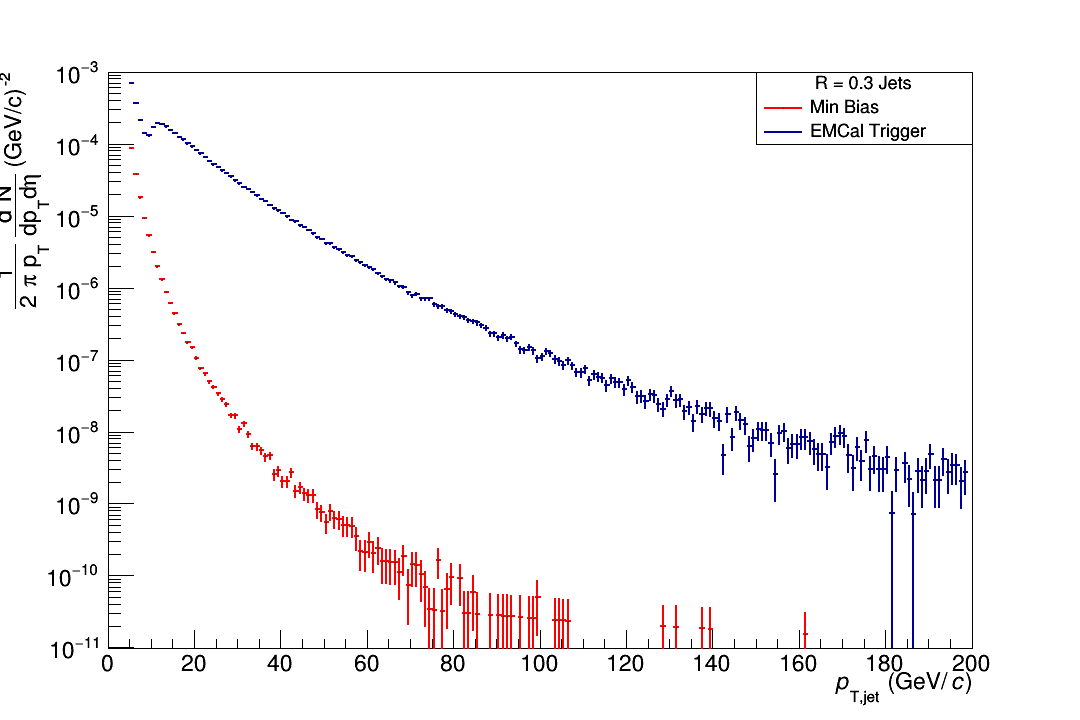
\includegraphics[width=8cm]{RawR03JetSpectra}
\centering
\caption{Raw inclusive R = 0.3 jet spectra from the 8 TeV Min Bias and EMCal triggered data}
\label{fig:rawjetR03}
\end{figure}
\begin{figure}[h]
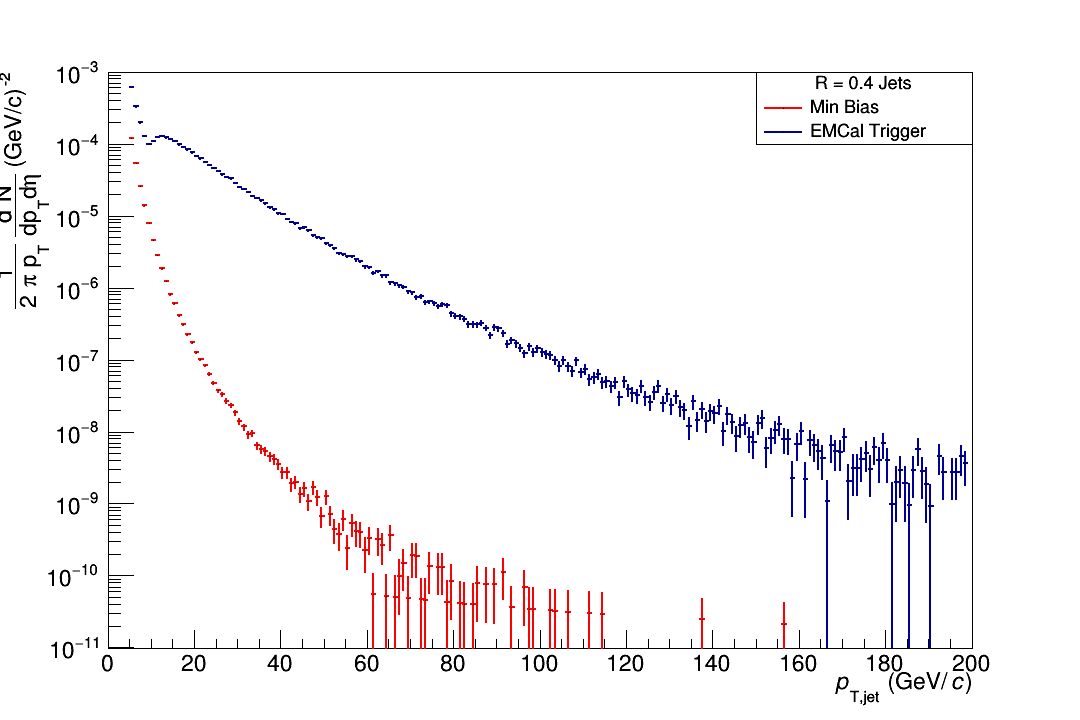
\includegraphics[width=8cm]{RawR04JetSpectra}
\centering
\caption{Raw inclusive R = 0.4 jet spectra from the 8 TeV Min Bias and EMCal triggered data}
\label{fig:rawjetR04}
\end{figure}

\noindent



\subsubsection{Event Selection}

During the 8 TeV data collection period, approximately 180 million Min Bias events were recorded, as summarized in table 5.1.  These events were separated into periods, which dictate the particular beam and detector configurations used during the data taking.  The 8 TeV data was broken into 7 periods, which werefurther broken into runs.  Runs represent an uninterrupted period of time during which the ALICE experiment is recording data. A run can be as short as 5 minutes or as long as 10 hours.  Runs were separated into `good' runs when both the TPC and EMCal were fully operational, `semi-good runs when a sector of the TPC was turned off but not around the region below the EMCal, and `bad' runs when a portion of the TPC was turned off directly below the EMCal or something else critically compromised the data.  This analysis only incorporated good and semi-good runs.

\begin{table}[hb]
\label{tab:RunSummary}
\begin{center}
\begin{tabular}[b]{|c|c|c|}
	\hline
	Period & \# of runs & \# of Min Bias events \\ \hline
	LHC12c & 89 & $\sim \,$24 M \\ \hline
	LHC12d & 140 & $\sim \,$62 M \\ \hline
	LHC12e & 5 & $\sim \,$2 M \\ \hline
	LHC12f & 56 & $\sim \,$15 M \\ \hline
	LHC12g & 8 & $\sim \,$0.4 M \\ \hline
	LHC12h & 159 & $\sim \,$75 M \\ \hline
	LHC12i & 40 & $\sim \,$3 M \\ \hline
	Total & 497 & $\sim \,$181 M \\ \hline

\end{tabular}
\end{center}
\caption{2012 8 TeV data taking period.}
\end{table}

Approximately 15\% of the data sampled was unusable due to malfunctions in TPC chambers, EMCal super modules, or the electronics of the EMCal or TPC.  The LHC12f  and LHC12g EMCal triggered data is not used in this analysis due to the trigger threshold being varied from the other periods.  Besides the bad runs excluded from each of the periods due to detector inefficiencies and the triggered LHC12f and LHC12g data, the rest of the 8 TeV data was used to generate the jet cross-sections in this thesis.  The LHC reported the integrated luminosity as $\mathscr{L}_{int} = 8.95 \, pb^{-1}$ during this data taking\cite{ALICE-PUBLIC-2017-002}.

\subsubsection{Monte Carlo Anchored Data}
Two Monte Carlo data sets, LHC15l2a1 and LHC15l2a2, which included a full GEANT4 simulation of the ALICE detector were produced by the ALICE collaboration and used for the Monte Carlo corrections in this analysis.   LHC15l2a1 uses a Pythia particle-level simulation embedded, or anchored, in a ALICE GEANT4 simulation with about 17 million Min Bias generated events.  LHC15l2a2 uses a PHOjet anchored data set consisting of about 21 million Min Bias triggered events.  Neither of these data driven Monte Carlos modeled the EMCal triggers.  Monte Carlo corrections of the EMCal triggered data suffered due to the lack of any simulations of the trigger and this is discussed in more detail later in this chapter.

\subsubsection{Event Selection Criteria}
For an event to be selected into a physics analysis it must pass a number of quality control tests.  For example, the LHC must be in a state of stable beams, cosmic rays must be excluded by only accepting tracks that originate from a vertex inside the detector, and the relevant detectors for a given analysis must be functioning as intended.  A number of these quality assurance, QA, were performed at the event level to exclude bad data, this thesis required the following criteria:

\begin{itemize}
  \item The event has a primary vertex reconstructed.
  \item The primary vertex occurs within a 10 cm window of the primary interaction point.
  \item The vertex resolution must be below 0.25 cm.
  \item The event passes basic pile-up checks based on the V0 and T0 signals.
\end{itemize}


A summary of the rejection reasons for an event are shown in Figure \ref{fig:eventqa}.  Most of the rejected events were excluded due to the event not satisfying the vertex requirements.

\begin{figure}[h]
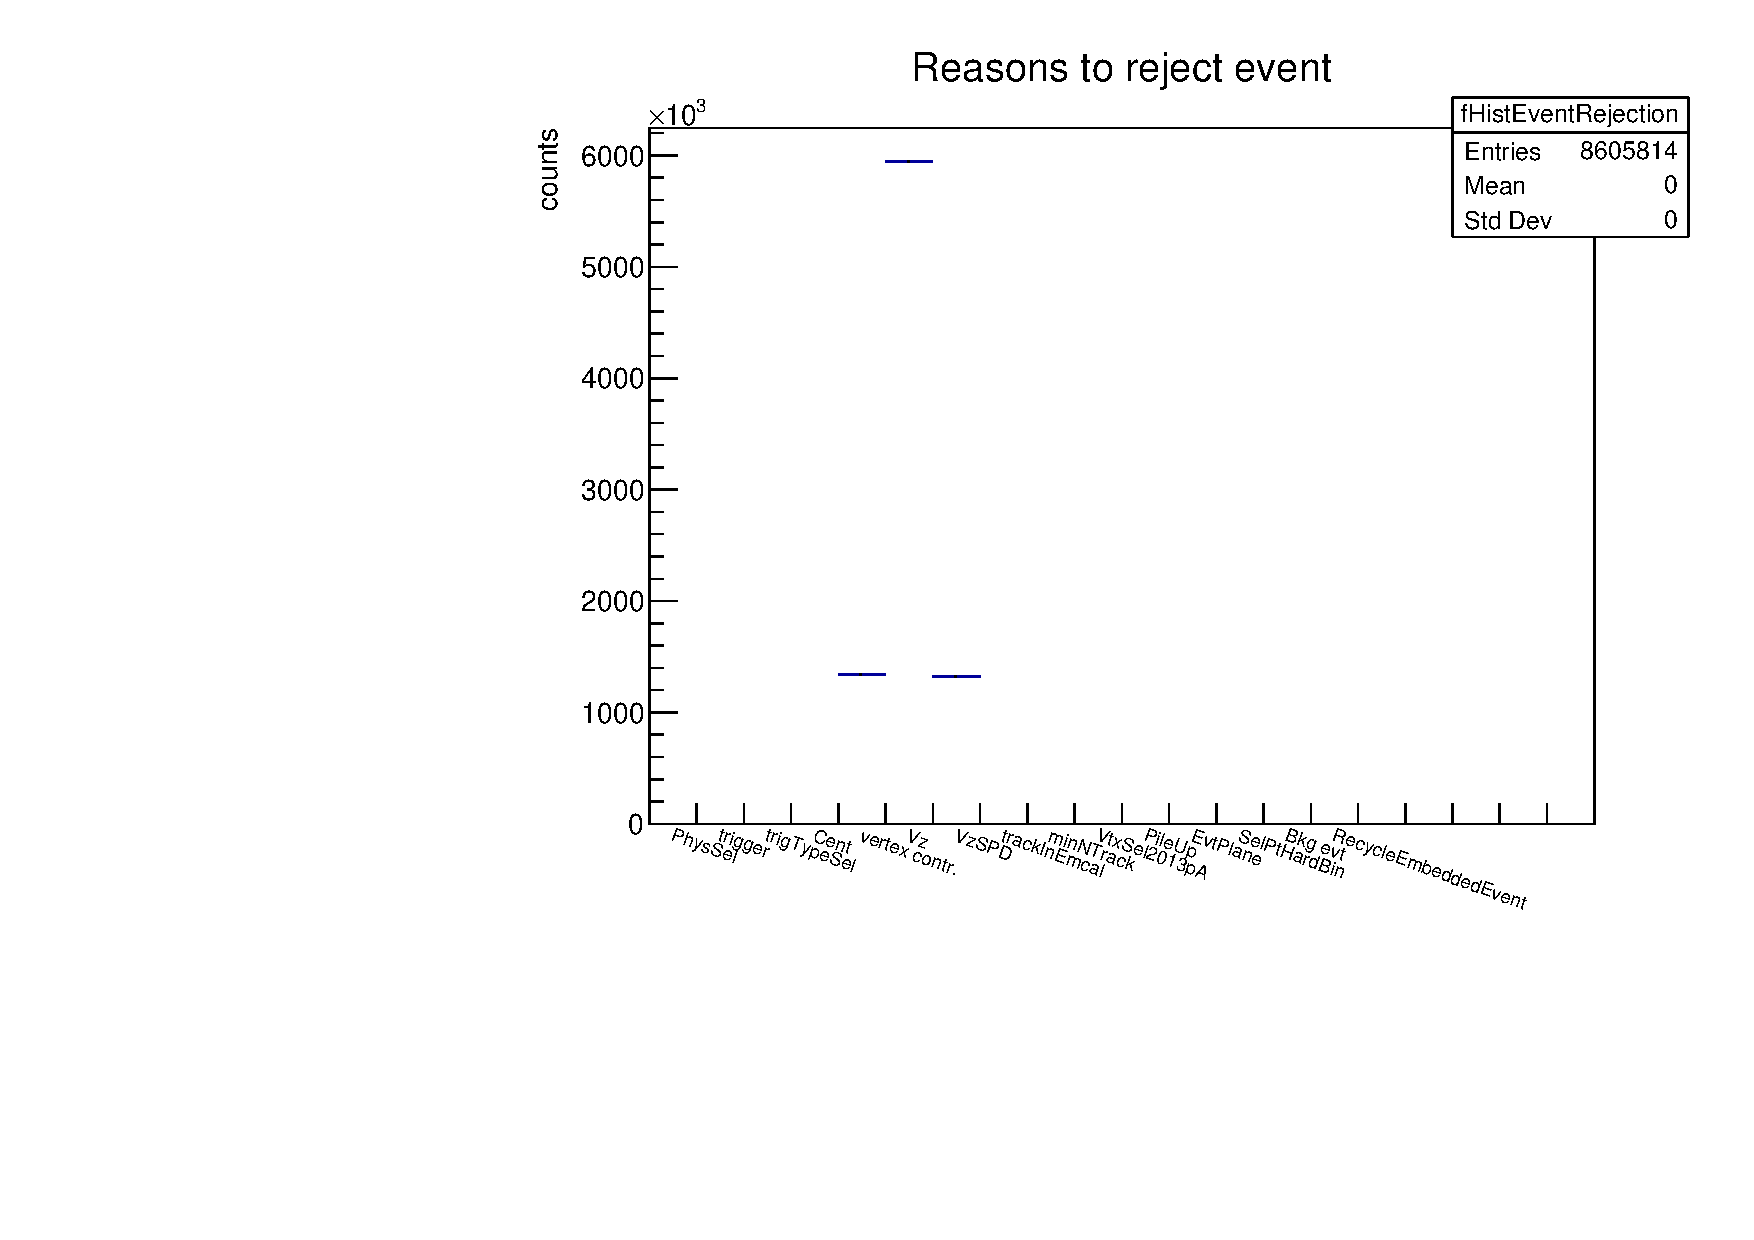
\includegraphics[width=8.5cm]{RejectionReasons}
\centering
\caption{Min Bias event rejection summary.}
\label{fig:eventqa}
\end{figure}

\begin{figure}[h]
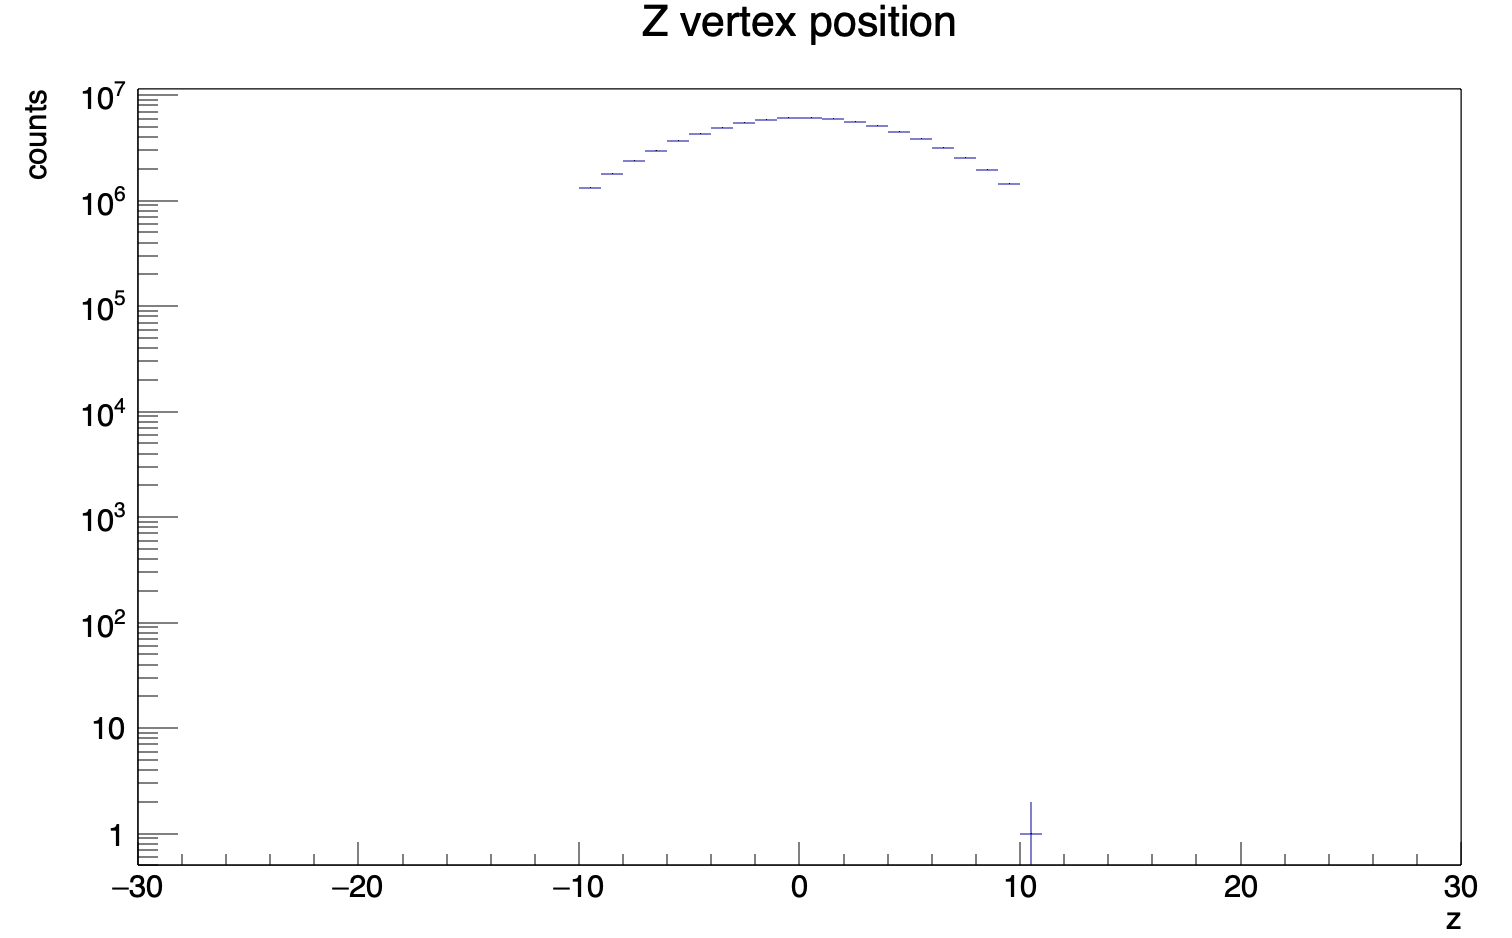
\includegraphics[width=8.5cm]{zvertex}
\centering
\caption{Vertex displacement from primary interaction point for accepted Min Bias events.}
\label{fig:vertrec}
\end{figure}


Figure \ref{fig:vertrec} shows the reconstructed vertex for the accepted Min Bias events after the QA was performed.  We see that the vertex distribution peaks at the primary interaction point as expected and that the distribution is well defined.  It should also be noted that a similar set of event QA was implemented to the EMCal triggered data and that the results were consistent with the Min Bias data.


\section{EMCal Triggered Data}

The EMCal triggered data for the 8 TeV data greatly extends the kinematic reach for the spectra.  This thesis looked at the two primary Level-1 triggers configured for the EMCal, the jet trigger (EJE) and the gamma (EGA) trigger\cite{Bourrion:2010js}.  Although both of the Level-1 triggers were investigated in this analysis, only the EGA trigger was ultimately corrected  and used for the final jet cross-sections and spectra.  

The EJE trigger utilizes a trigger patch consisting of 32 x 32 EMCal towers sliding by 8 towers until a patch is reconstructed that meets the minimum predefined trigger energy threshold.  Once this threshold is surpassed the event is recorded and tagged as a EJE triggered event.  A similar procedure is followed for the EGA trigger, but with a smaller patch region of 4 x 4 towers with a sliding window of 2 towers and its own predefined trigger threshold.  

The bump at low-$p_{T}$ seen in Figures \ref{fig:rawjetR02} - \ref{fig:rawjetR04} is the trigger turn on curve and the peak corresponds to the trigger threshold for the EGA trigger.  Ideally, a jet in the EMCal acceptance should fire the EJE trigger and the EGA should fire due to the presence of a photon or electron.  Since the triggers increase the yield of jets measured, the spectra from the triggered data must be corrected and downscaled.  In order to calculate these corrections two pieces of code were developed.  One reconstructs the EMCal and trigger patch geometries and allows a user to set the trigger thresholds for the EJE and EGA triggers to values used during a given LHC data taking period.  The other code attempts to match the reconstructed trigger center to the jet center.  The trigger centroid is obtained using a weighted means method by summing over the number of towers in a patch and dividing this quantity by the energy in each tower.  Both sets of codes are publicly available tp the public and are officially part of ALICE software framework.  For this analysis I used a lose requirement that the EGA or EJE patch center were within the radius of a given jet.  The geometrical matching requirement followed a simple quadratic relationship,,

\begin{equation}
\sqrt{ ( \phi_{jet} - \phi_{EGA, patch} )^{2} + ( \eta_{jet} - \eta_{EGA, patch} )^{2}}  \leq R_{jet} .
\label{eq:triggermatch}
\end{equation}

\begin{figure}[h]
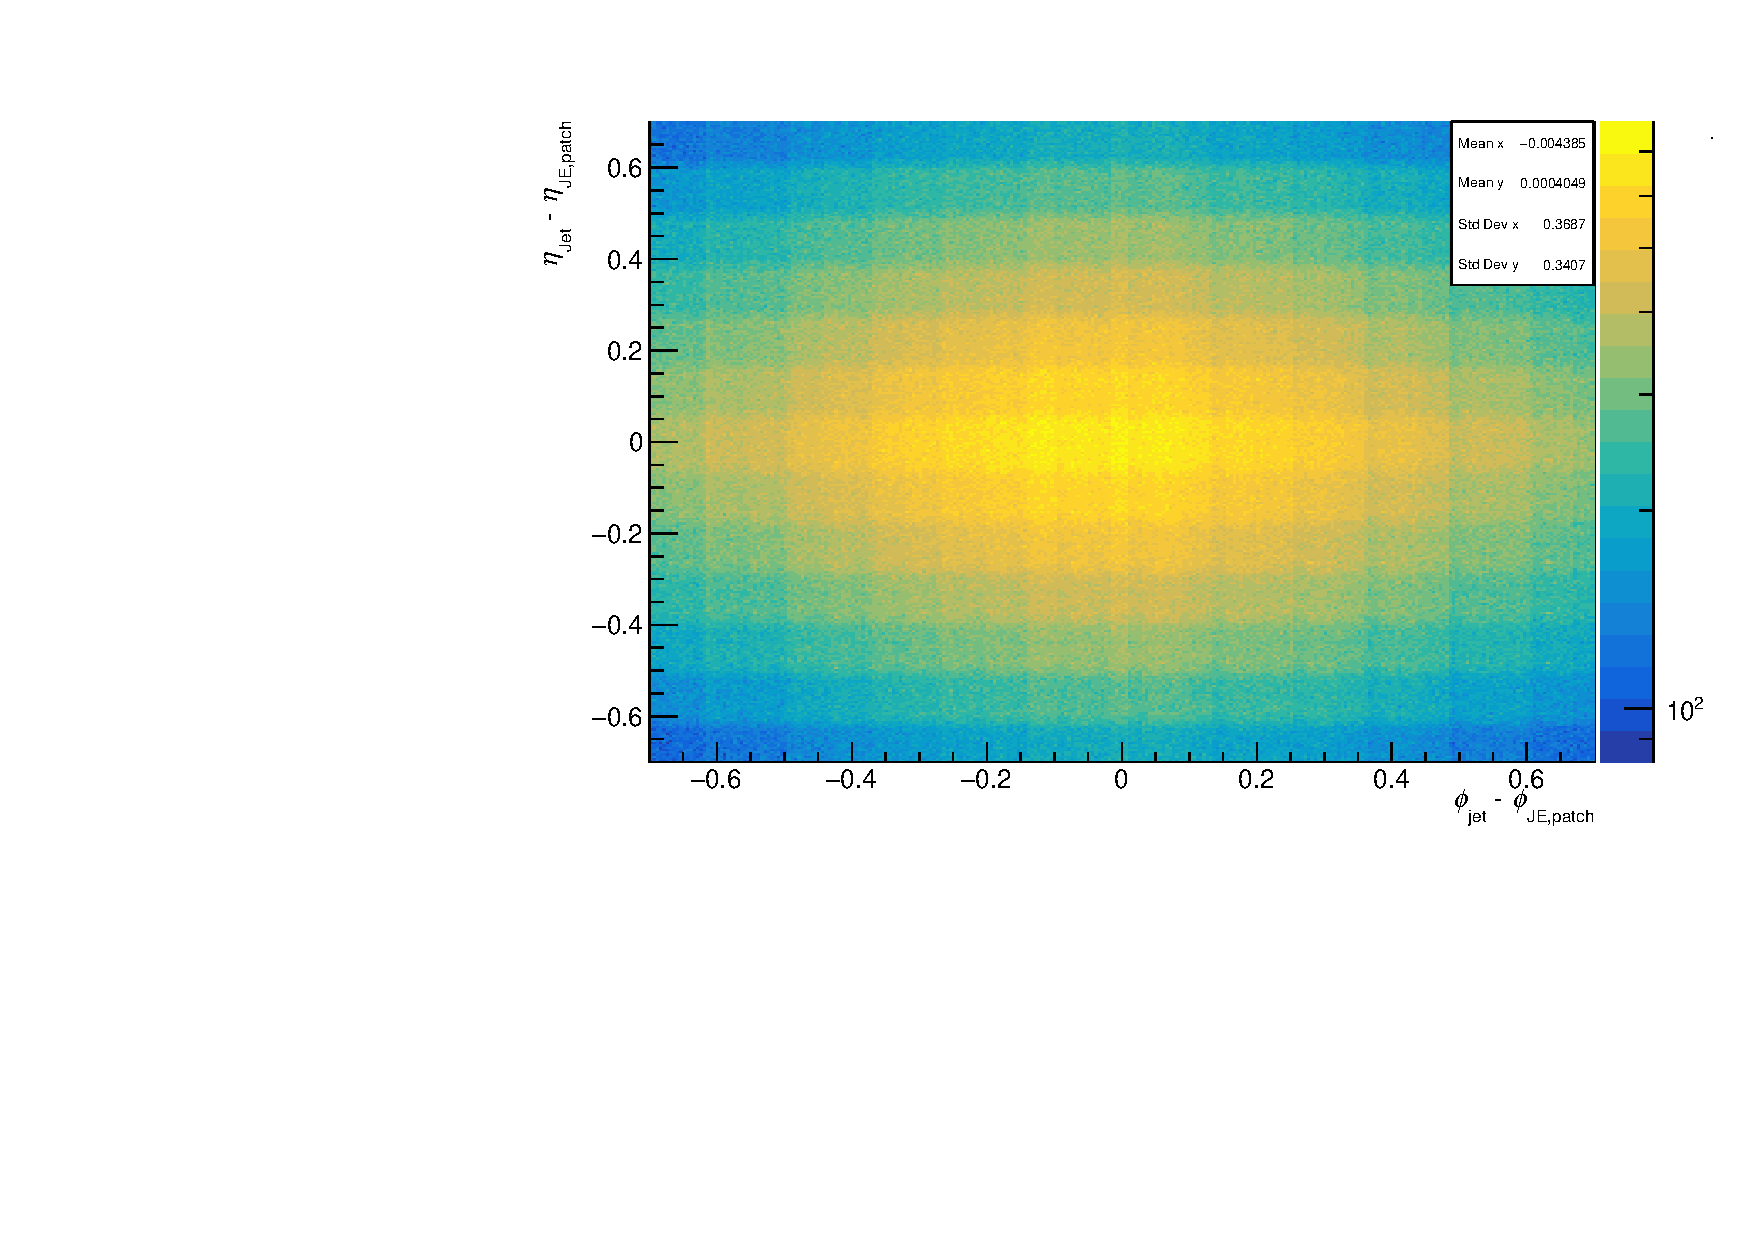
\includegraphics[width=10cm]{DistanceJetEJER02}
\centering
\caption{Distance to closest reconstructed EJE patch to R = 0.2 jet with the Min Bias Pythia Monte Carlo.}
\label{fig:DisJetEJE}
\end{figure}

\begin{figure}[h]
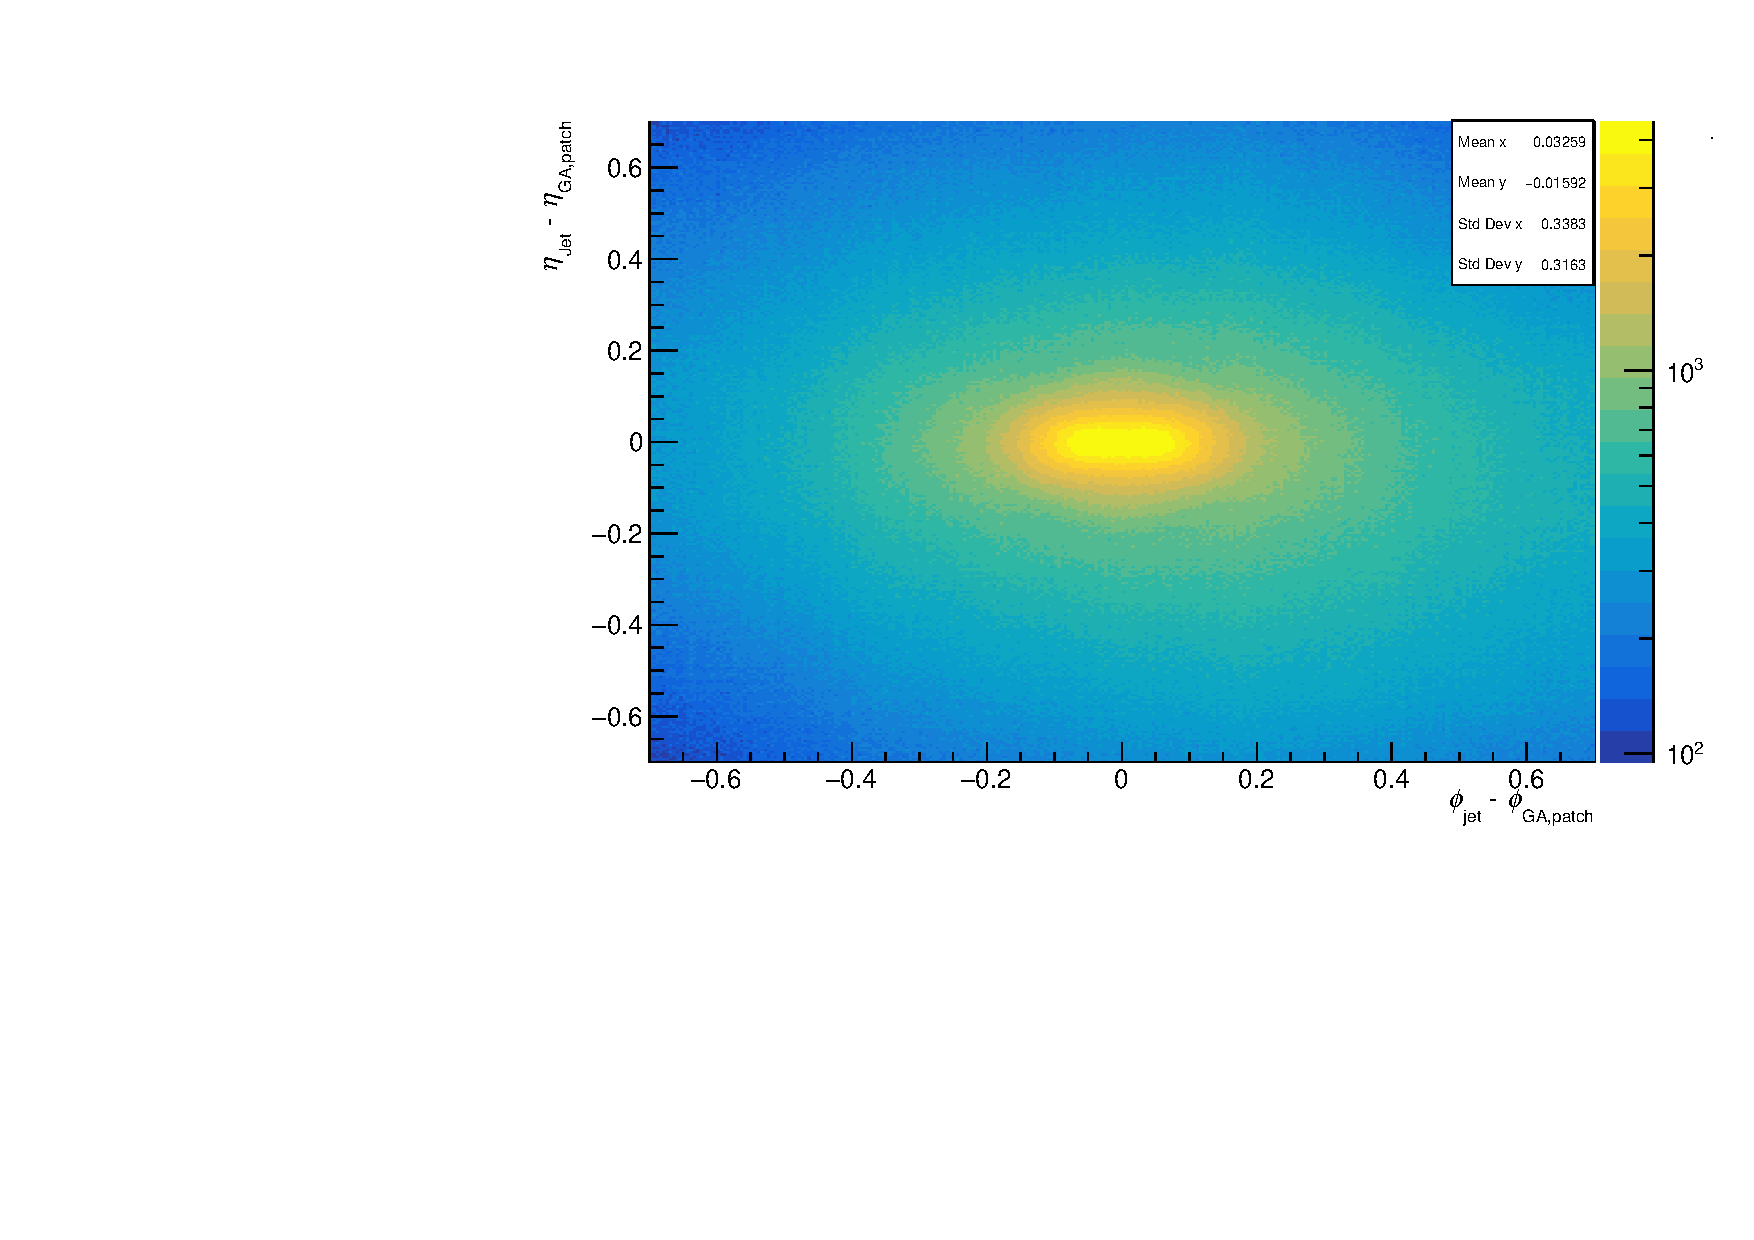
\includegraphics[width=10cm]{DistanceJetEGAR02}
\centering
\caption{Distance to closest reconstructed EGA patch to R = 0.2 jet with the Min Bias Pythia Monte Carlo.}
\label{fig:DisJetEGA}
\end{figure}

\noindent
Figures \ref{fig:DisJetEJE} and \ref{fig:DisJetEGA} show the distance between a reconstructed jet and its closest reconstructed EMCal trigger patch for R = 0.2 jets in the Pythia Monte Carlo.  Since a trigger patch may be fired if two or more jets are within the geometric area of the trigger patch this could lead to double counting.  In order to correct for this, the jet spectra from the triggered data is scaled by the number of triggers, $N_{trig}$, fired that fell within the jet.  We can see that with the EGA trigger that the peak of the distribution is within the jet radius of R = 0.2 while with the EJE trigger the distribution is more uniformly distributed.  The EJE distribution can be accounted for the fact that the EJE trigger is large enough to have multiple jets matched to EJE trigger patch or vice-versa.  The fact that the distribution of seen in Figure \ref{fig:DisJetEJE} spans such a large area means that the jet center was typically not well correlated with the center of the EJE patch and this is the primary reason why the inclusion of the EMCal jet triggered data was abandoned for this thesis.

Once this correction was implemented, the triggered data was then downscaled in order to combine it with the Min Bias data.  The downscale correction factors, shown in Figure \ref{fig:EMCalDownScale}, wee obtained by taking the ratio of the EMCal jet spectra to the Min Bias jet spectra and fitting the plateau region to a line.  At low-$p_{T}$, below $\sim$40 GeV,  the two data sets do not scale linearly and so the EMCal data below 40 GeV was ignored.


\begin{figure*}[t!]
$\begin{array}{rl}
    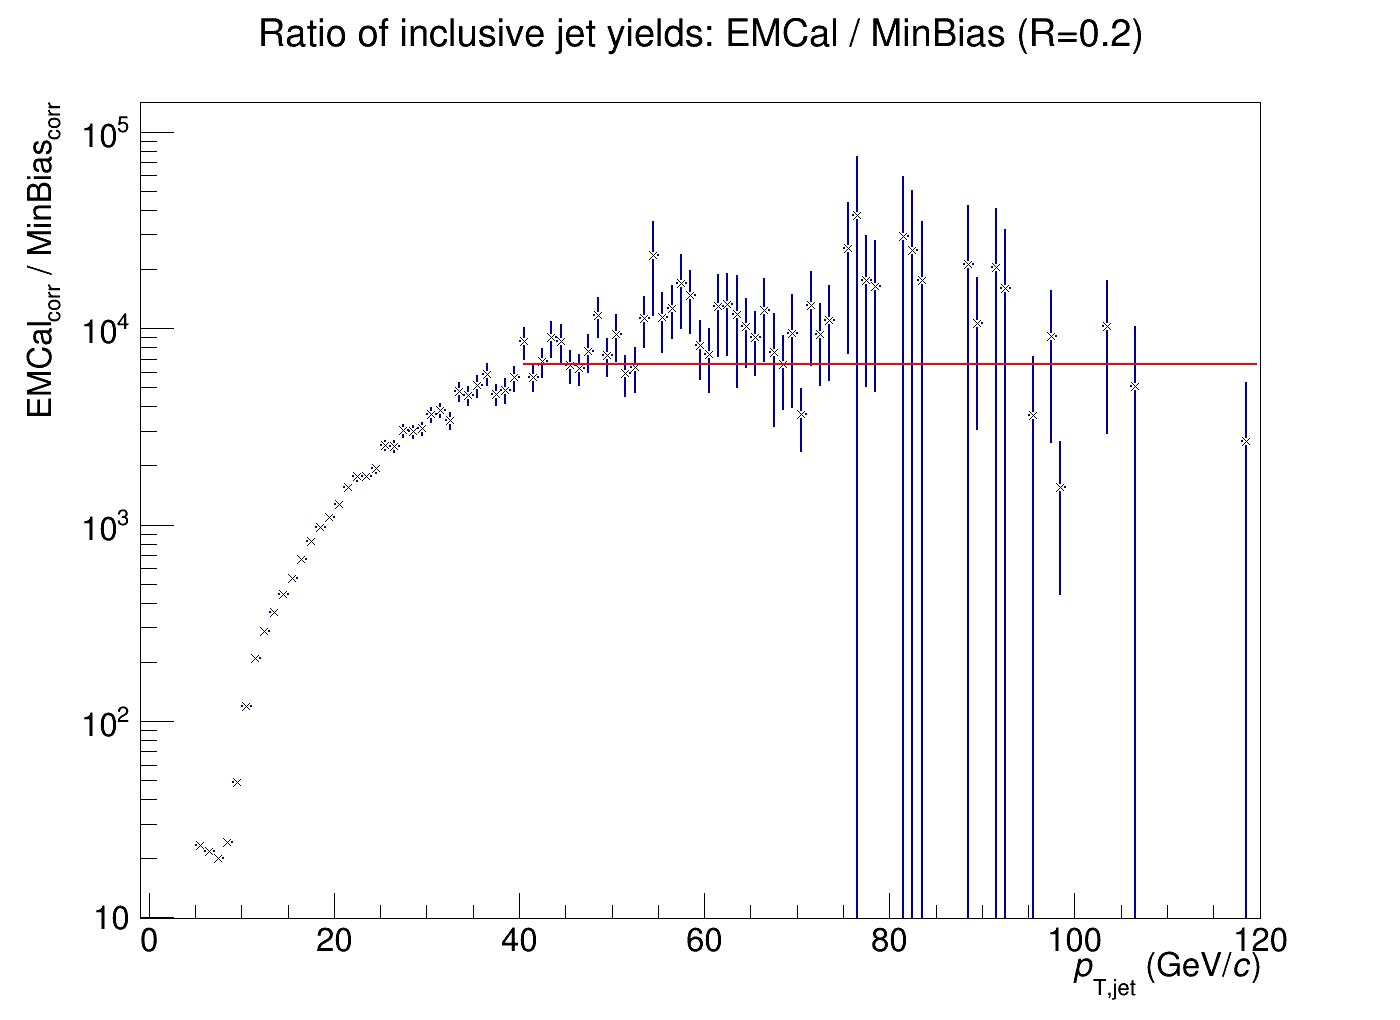
\includegraphics[width=0.5\textwidth]{R02TriggerYields} &
    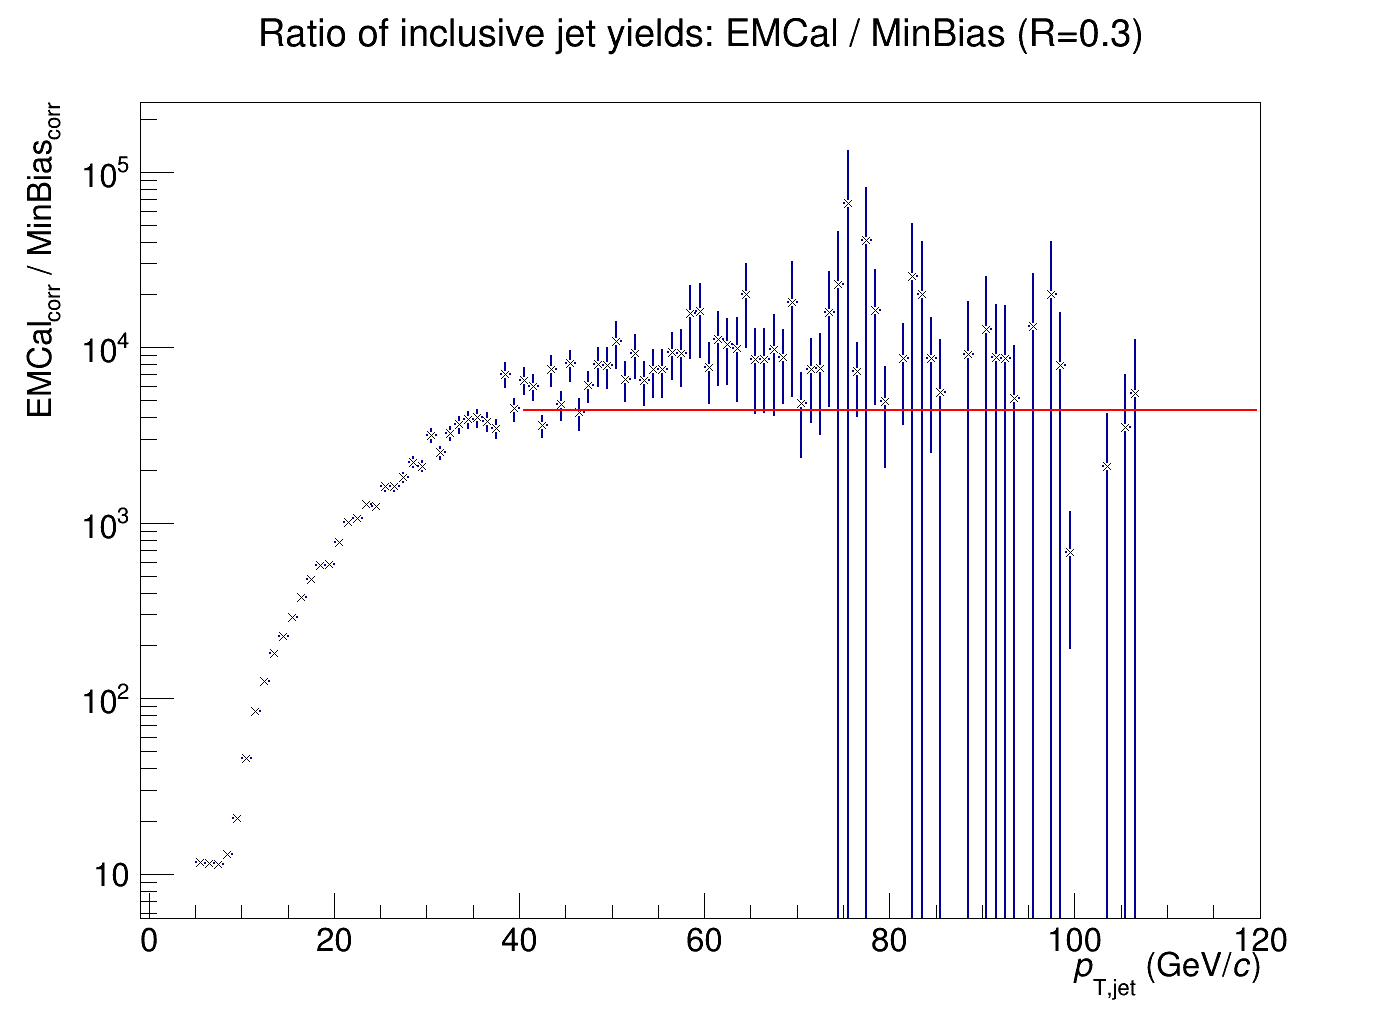
\includegraphics[width=0.5\textwidth]{R03TriggerYields}\\
    \multicolumn{2}{c}{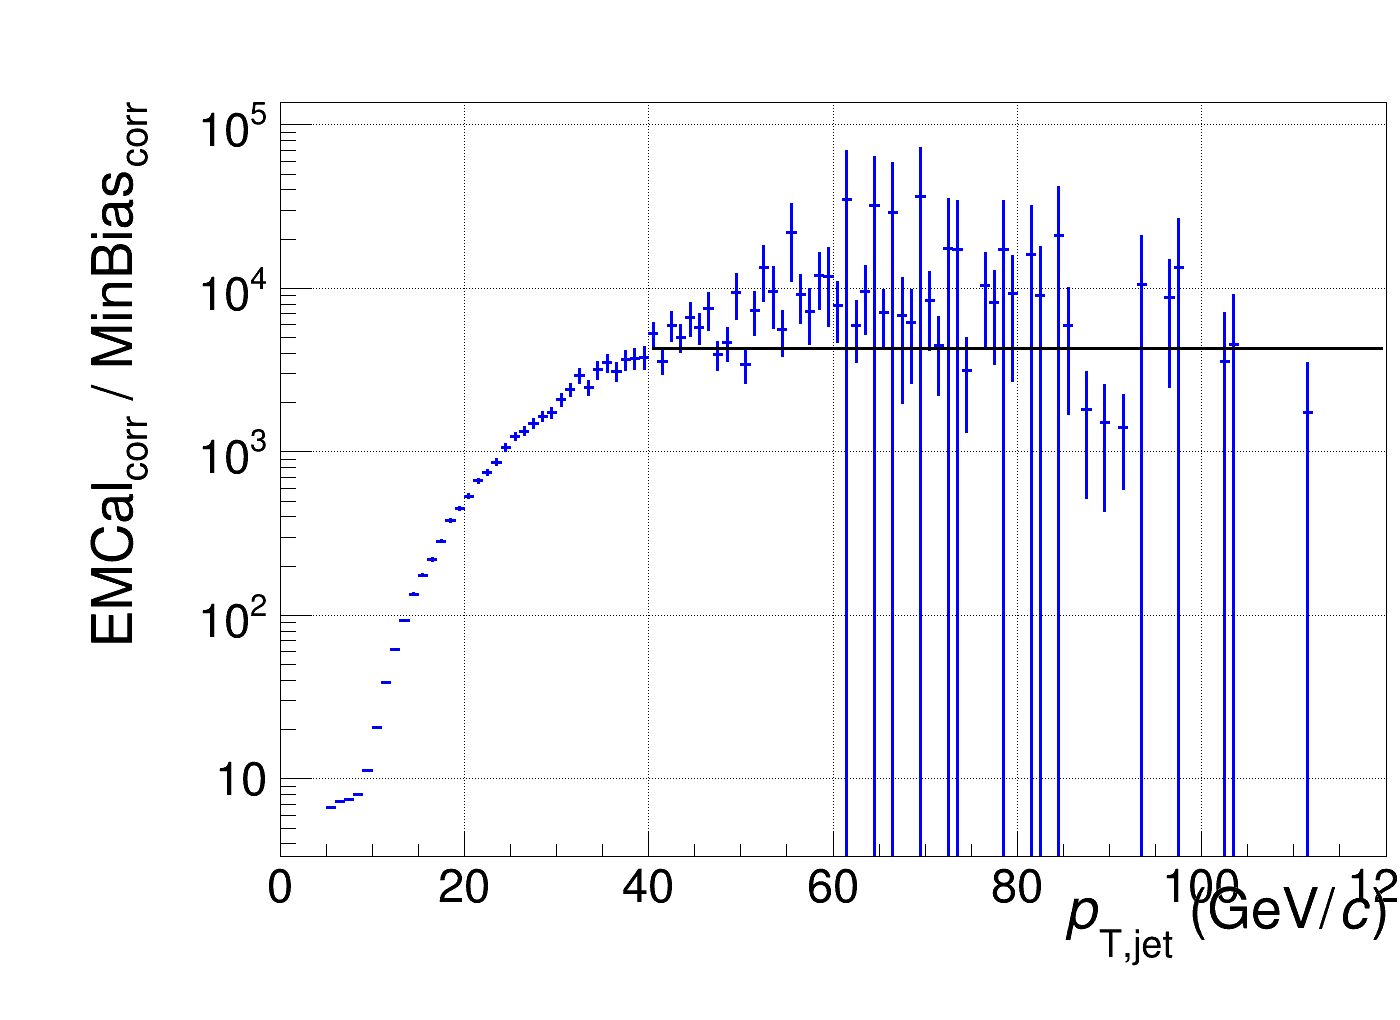
\includegraphics[width=0.5\textwidth]{R04TriggerYields}}
\end{array}$
\caption[EMCal triggered data correction factors for R=0.2, R=0.3, and R=0.4 jets.]{\label{fig:EMCalDownScale}EMCal triggered data correction factors for R=0.2, R=0.3, and R=0.4 jets.}
\end{figure*}

These two corrections allow for the EMCal data to be combined with the Min Bias data.  It should be noted that the scale factors were after the Monte Carlo corrections were implemented which is discussed further on in this chapter.  With the data scaled and combined the next sections will detail more of the QA performed for this analysis.


\section{Cluster Selection}
Corrections were performed on EMCal cells including the removal of hot and dead towers (bad channels) based on the average occupancy and energy of the towers, calibrations to cell timing caused by the physical layout of the EMCal (such as differences in cabling length), and an energy calibration based on the $\pi^{0}$ mass.  After these corrections were applied, the towers were grouped together into clusters using the v2 algorithm.  The v2 algorithm has a minimum tower seed, $E_{seed} = \,$ 300 MeV, after which all adjacent towers with a minimum energy, $E_{cell} \geq \,$ 100 MeV, are iteratively added until a local minimum is reached.  The cluster energy is the sum of the seed and grouped neighbor tower energies.  Figure \ref{fig:badchannel} shows a bad channel map after removing the hot and dead towers from a typical run.  The $\phi$ distribution is segmented into 5 parts representing the five super modules of the EMCal.

\begin{figure}[h]
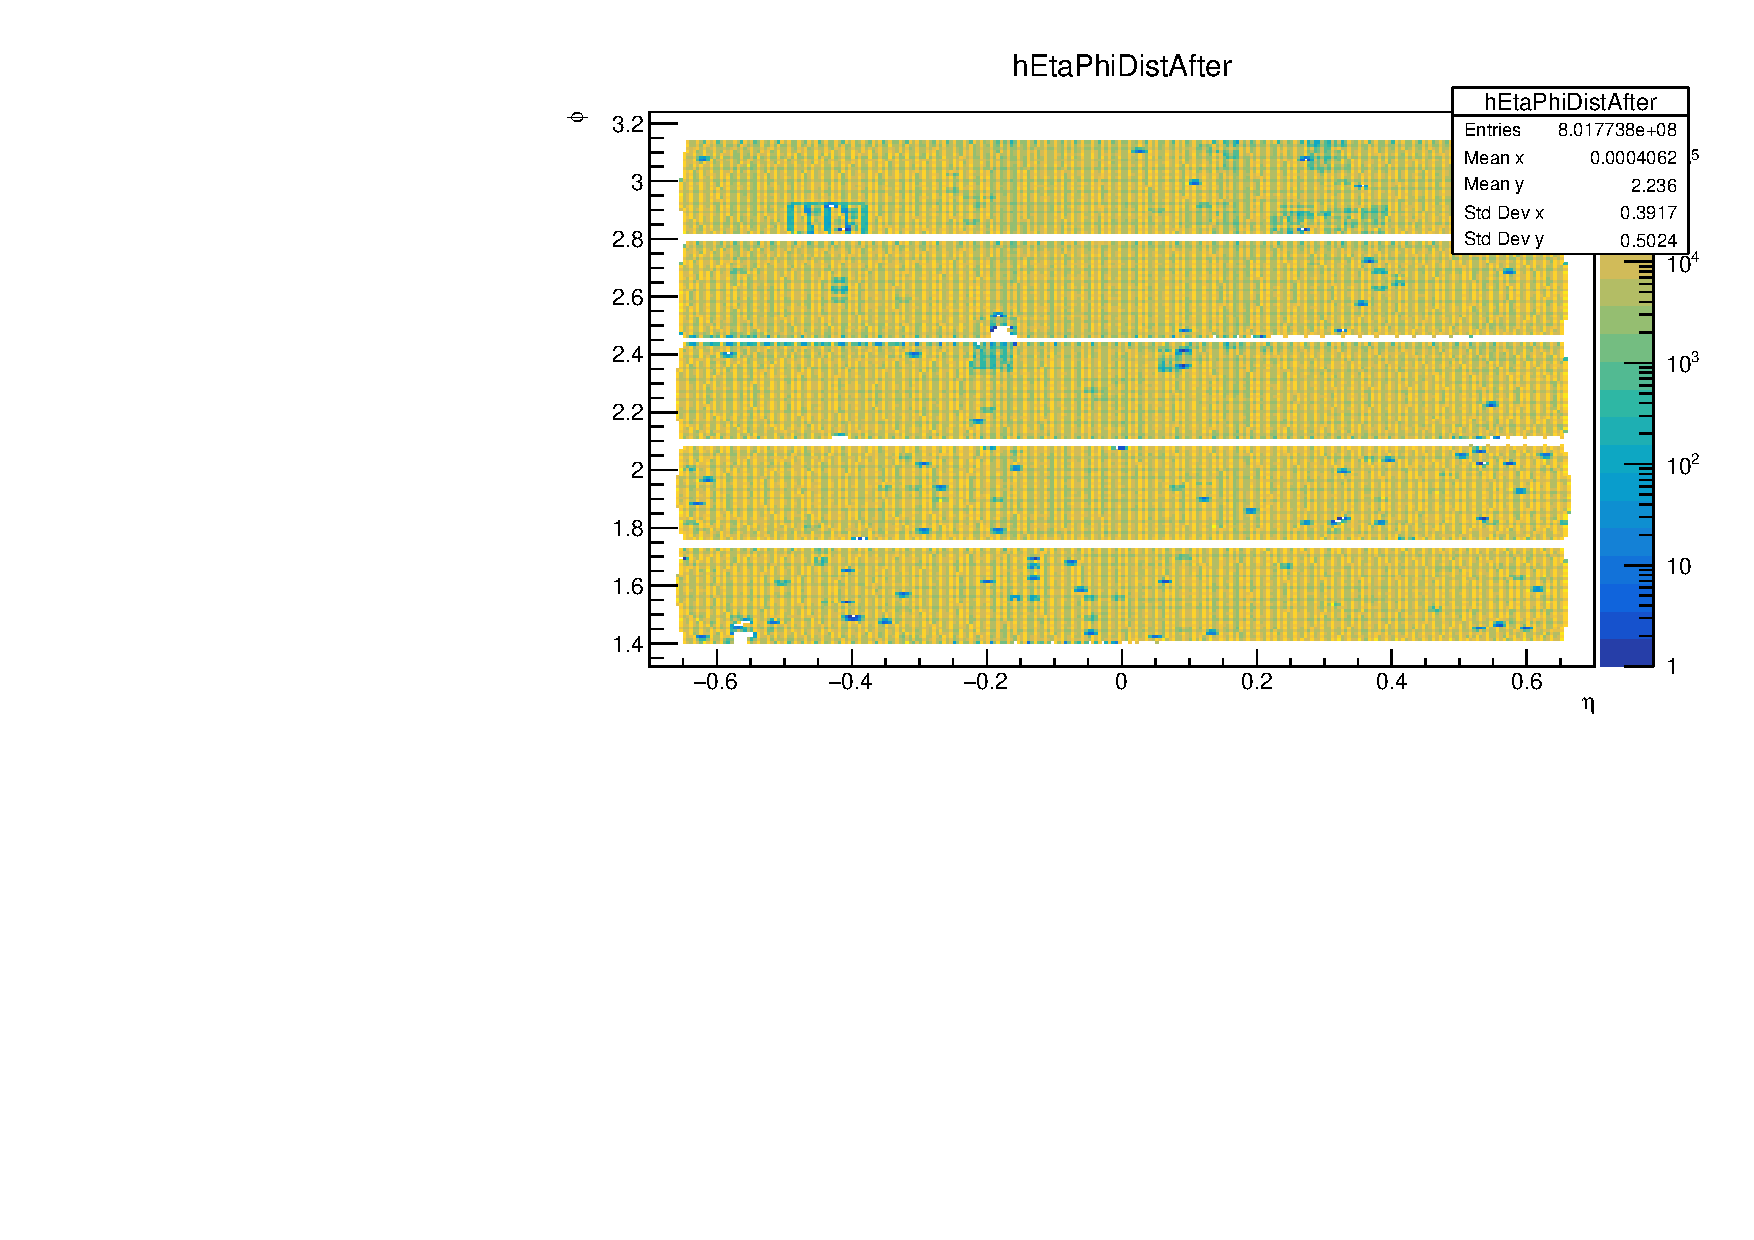
\includegraphics[width=14cm]{BadChannelMap}
\centering
\caption{EMCal cell occupancy after bad channels removed.}
\label{fig:badchannel}
\end{figure}

After the cells are clustered together the clusters are corrected for exotics.  This correction was performed by cutting all clusters with a $F_{cross} \geq \,$ 0.97, where

\begin{equation}
F_{cross} = 1 - \frac{ E_{cross} }{ E_{cell} },
\label{eq:Fcross}
\end{equation}

\noindent
where $E_{cross}$ is the sum of the four cells sharing a full edge with the leading cell and $E_{cell}$ is the center pixels energy.  The main source of exotic clusters in the EMCal is most often due to a hadron hitting the Avalanche Photodiode (APD) in a tower.  This will concentrate the energy of the cluster into a single tower while the adjacent towers will contain only a small fraction of the cluster energy.  The clusters were removed before jet finding occurred as they are an artifact of the detector performance.

The EMCal is optimized to measure the energy of electrons and photons as they tend to fully shower inside the EMCal structure.  Hadrons are detected by the EMCal, but will only shower a fraction of their intrinsic energy.  A hadronic correction was performed in order to account for this missing energy due to the partial hadron shower.  Charged tracks from the outer layer of the TPC were propagated to the EMCal, by fitting the trajectory of the track to a curve, and the of the clusters and tracks were matched together geometrically.  Figure \ref{fig:EMChadetaphi} shows the distance between the centroid of a cluster in the EMCal and the nearest track propagated from the TPC.  Hadrons are identified by requiring the matched distance to be, $\sqrt{ \Delta\phi^{2} + \Delta\eta^{2} } \leq \,$ 0.015, which is within one EMCal tower distance.

\begin{figure}[h]
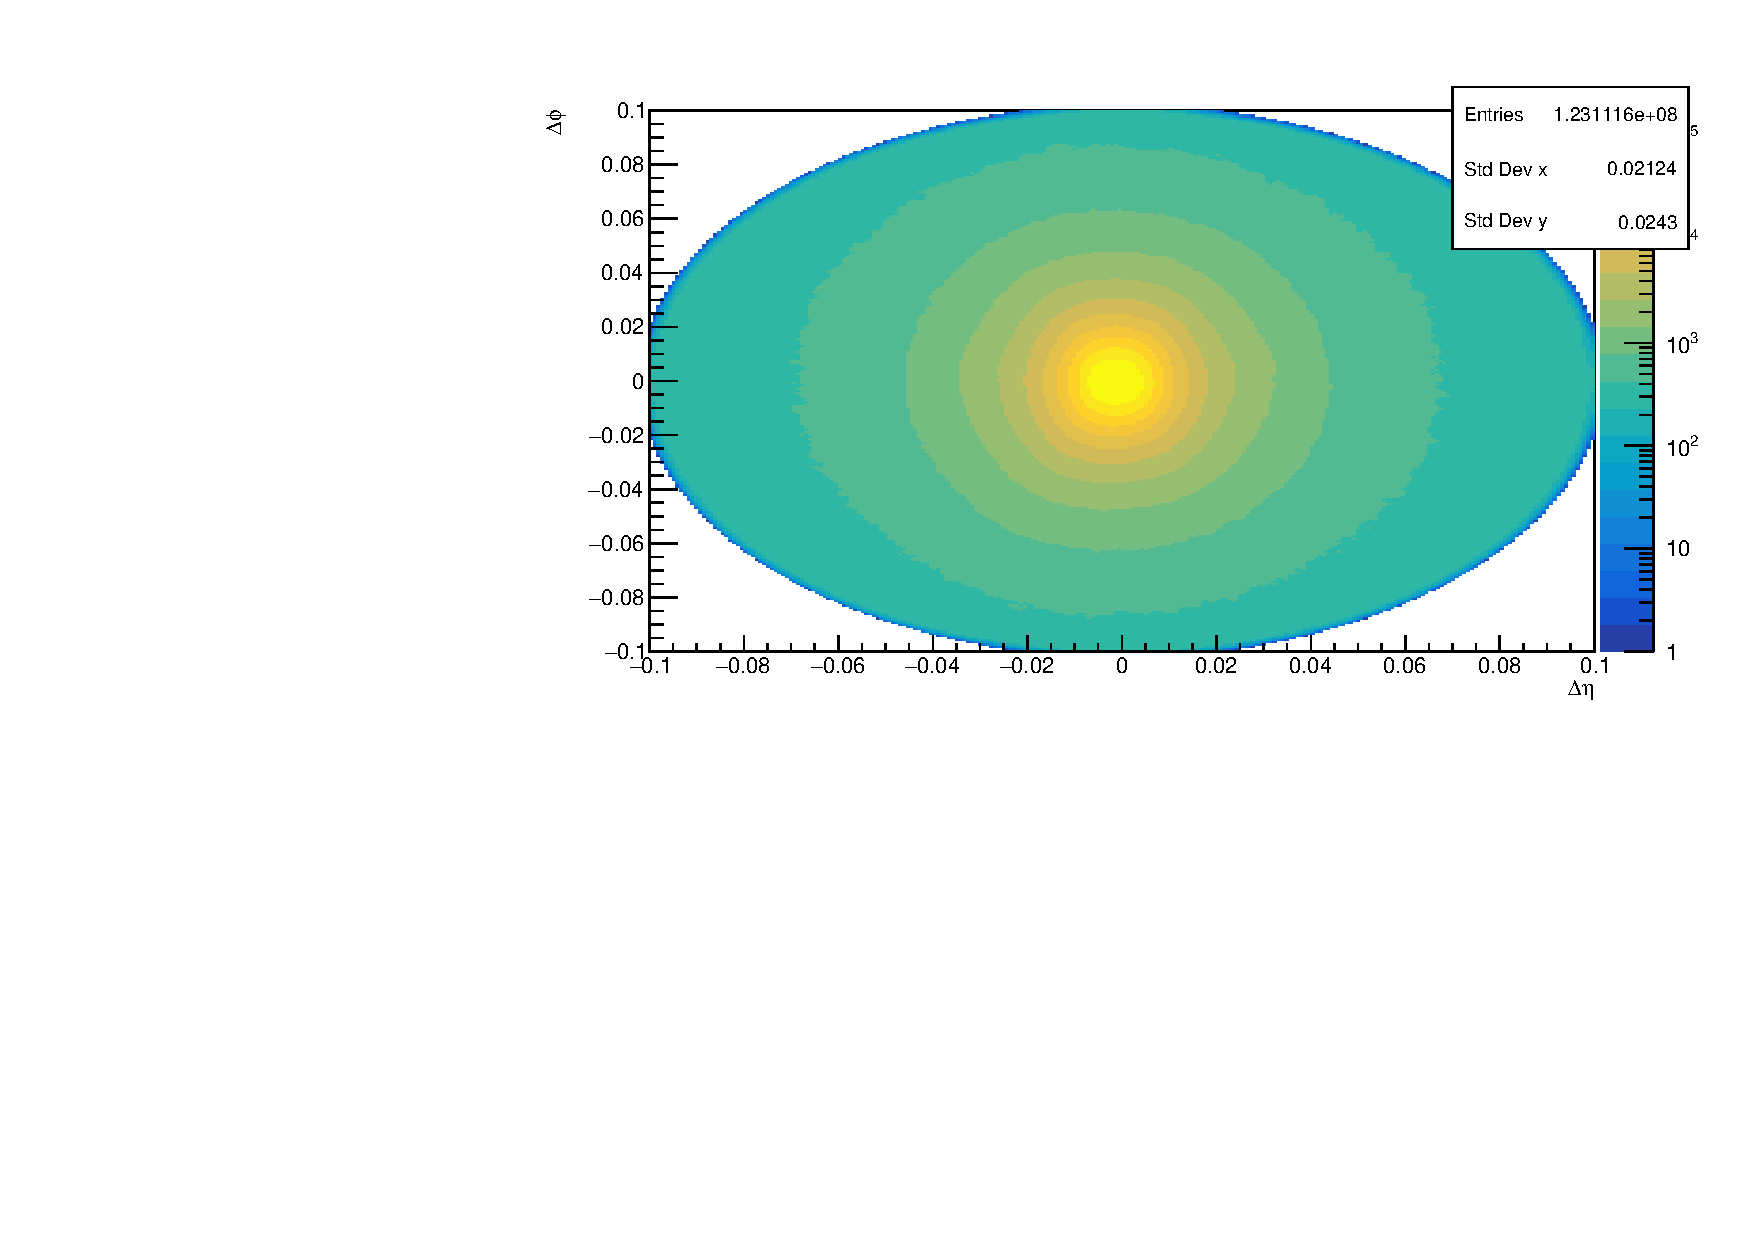
\includegraphics[width=12cm]{hadronetaphi}
\centering
\caption{Matched track-cluster distance.}
\label{fig:EMChadetaphi}
\end{figure}

\noindent
Corrections for the double counting from hadrons is based on correcting the EMCal cluster energy by a weight function,

\begin{equation}
E_{corr} = E_{clust} - f_{sub} \times \sum p ,
\label{eq:HadCorr}
\end{equation}

\noindent
where $\sum p$ is the magnitude of the 3-momentum of the hadron and $f_{sub} = 1$ is the nominal value for the weight.  If $E_{corr} \leq 0$ the cluster was removed, this may be caused by cluster pile-up and only accounted for a small fraction of the clusters.  In order for a cluster to be accepted $E_{corr} \geq \,$ 300 MeV was required, because a minimum ionizing particle (MIP) will on average deposit 280 MeV in the EMCal.  

A final cut was performed on the cluster timing, obtained from the T0, the time of arrival for a particle is shown on the y-axis of Figure \ref{fig:EMCaltime}.  

\begin{figure}[!h]
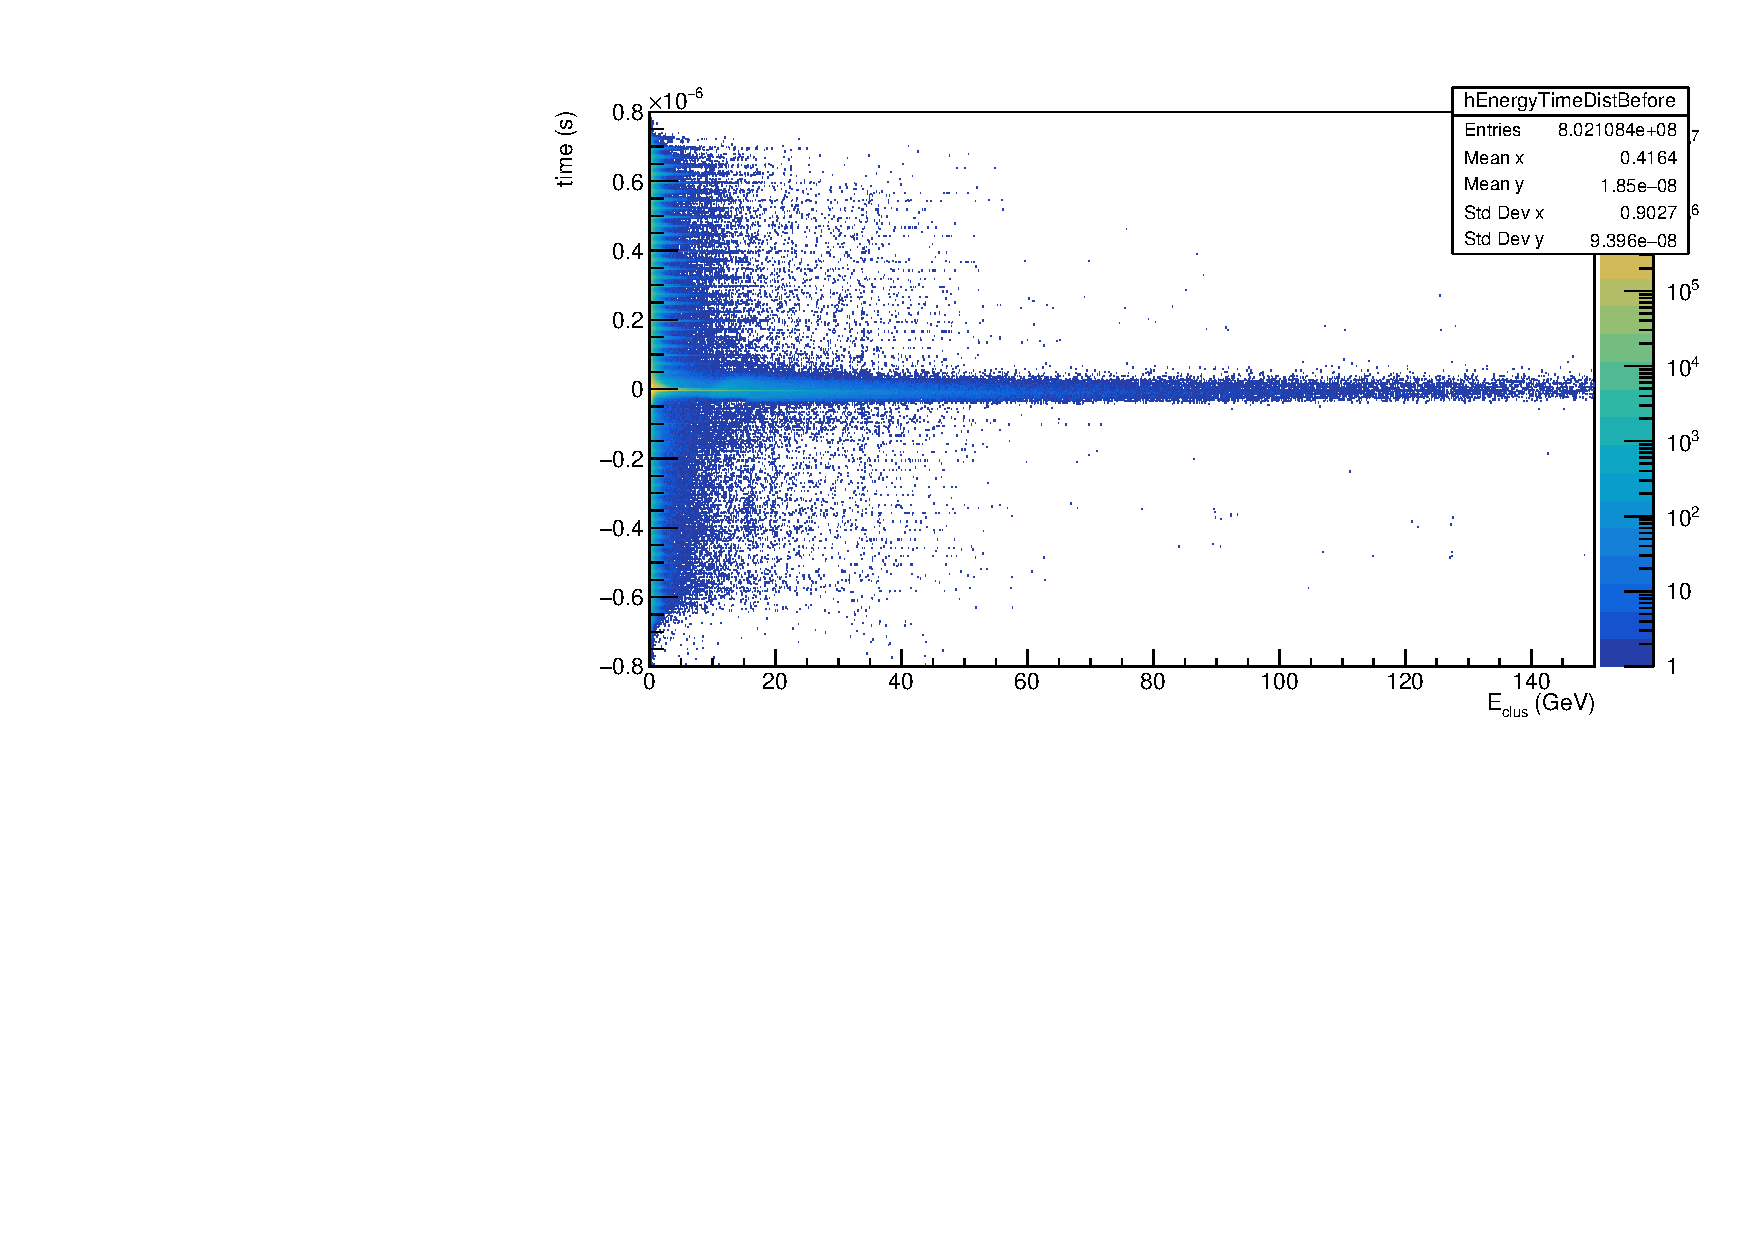
\includegraphics[width=11cm]{timming}
\centering
\caption{EMCal cluster time distribution before cuts.}
\label{fig:EMCaltime}
\end{figure}


Cutting on the cluster time is done in order to readout only the particles created from an event and to limit the contamination due to slower particles from previous events.  The main source of the slow moving particles are neutrons and $K_{L}^{0}$ and this analysis limited cluster time to $t_{clus} \, \epsilon \,$ [-50 ns, 100 ns].


\begin{figure}[h]
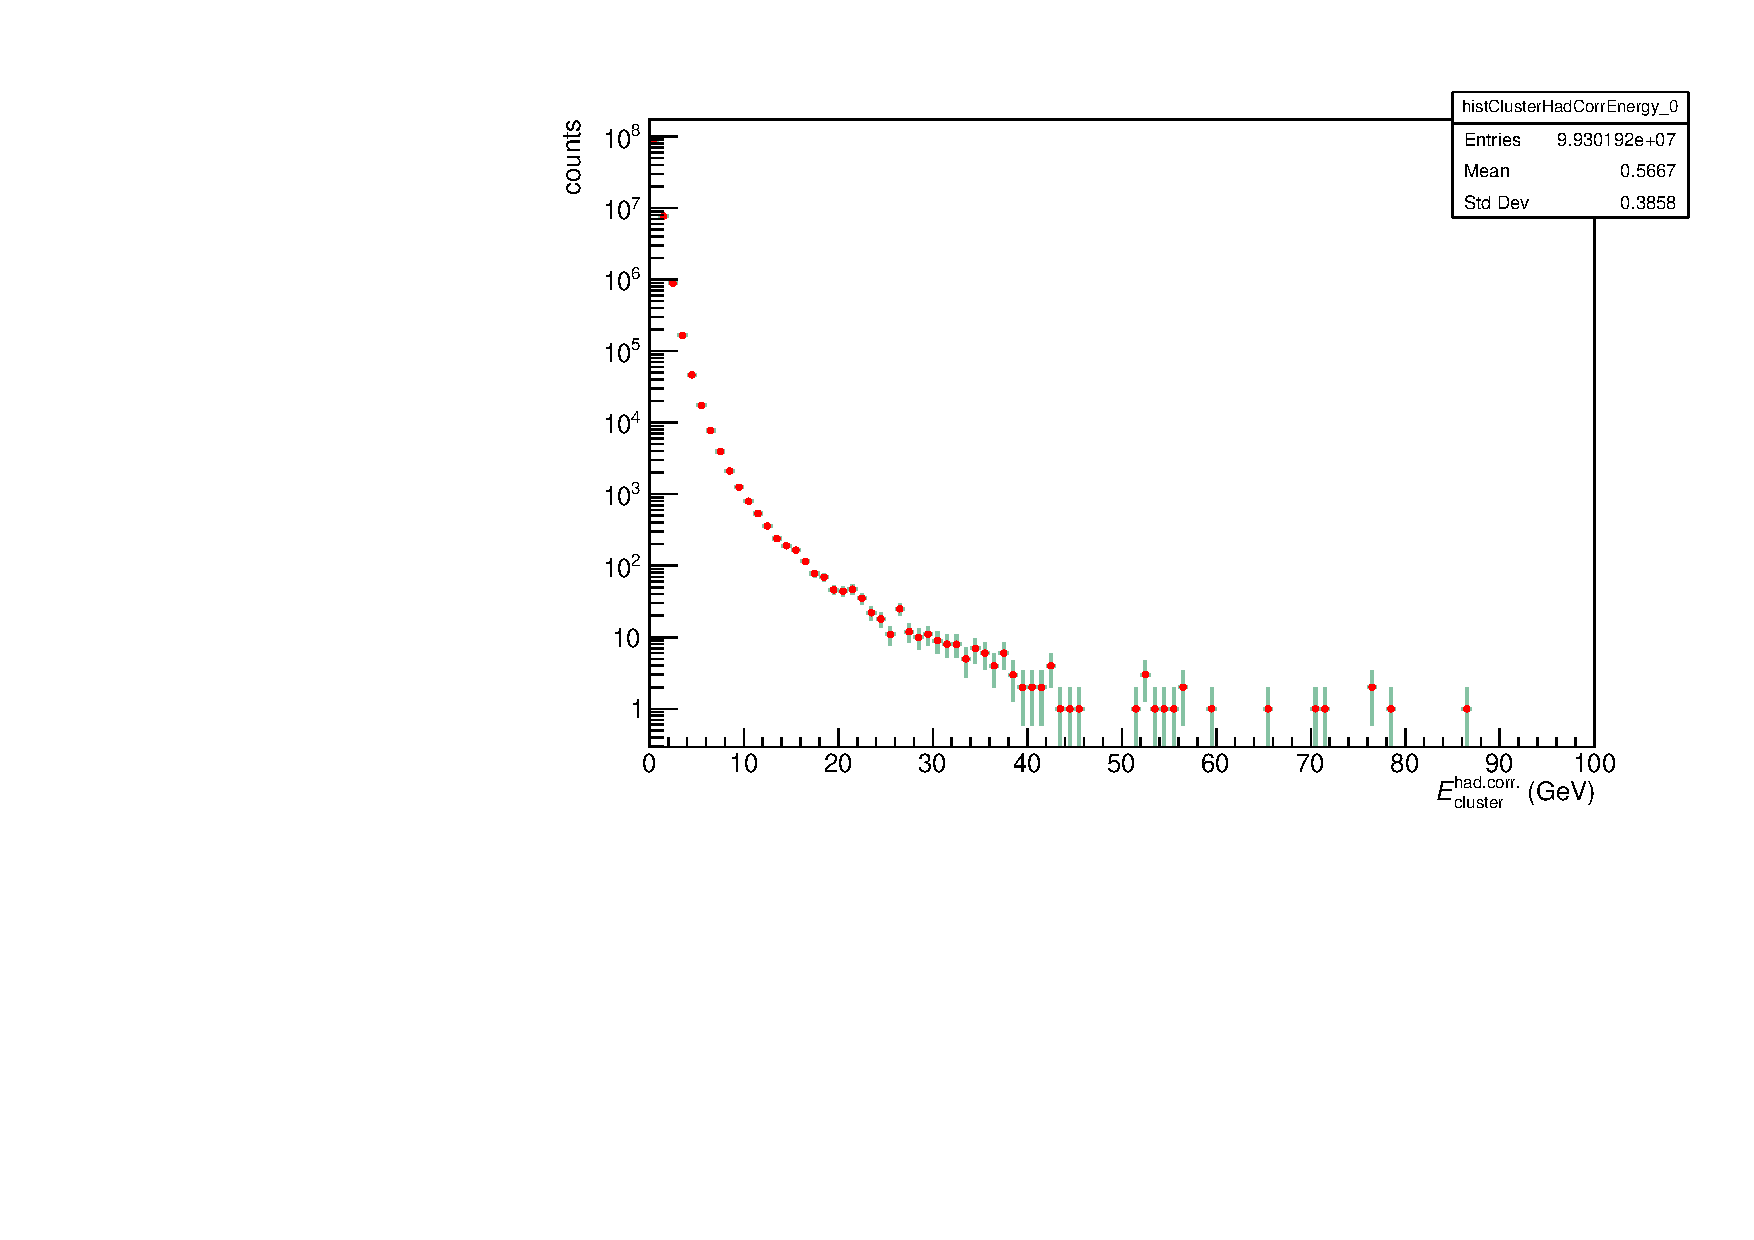
\includegraphics[width=8cm]{Eclusfinal}
\centering
\caption{Corrected EMCal cluster yield.}
\label{fig:EMCalfinal}
\end{figure}
\newpage

Figure \ref{fig:EMCalfinal} shows the final cluster energy distribution with all the cuts and corrections previously discussed applied, and makes up the set of clusters over which the jet finding was performed.  The same cuts and corrections were applied to the EMCal triggered data.

\section{Track Selection}

Tracks were reconstructed in the TPC using a Kalman filtering which helps alleviate any corrections needed due to multiple scatterings, dead sectors, etc.  Jet finding was performed using `hybrid' tracks.  Hybrid tracks consist of two track sets, the first being all tracks with at least one hit in the SPD (Global), and the second set being all tracks that can be constrained to the primary vertex (Complimentary).  The reconstruction of a signal from the ITS and TPC form good tracks if the $\chi^{2}/NDF$, chi-square per degrees of freedom, is required to be less than 4 in the TPC and $\chi^{2}$ is required to be less than 36 in the ITS. For this analysis, the minimal $p_{T, track}$ was 150 MeV/c and the track was constrained to the TPC acceptance: - 0.9 $\leq \eta \leq$ 0.9 and 0 $\leq \phi \leq$ 2$\pi$, shown in Figure \ref{fig:Hybridtracketaphi}.  The spatial distributions of the hybrid tracks remain relatively flat as expected in the 8 TeV data set for good and semi-good runs.

\begin{figure}%
    \centering
    \subfloat[Hybrid Track $\eta$]{{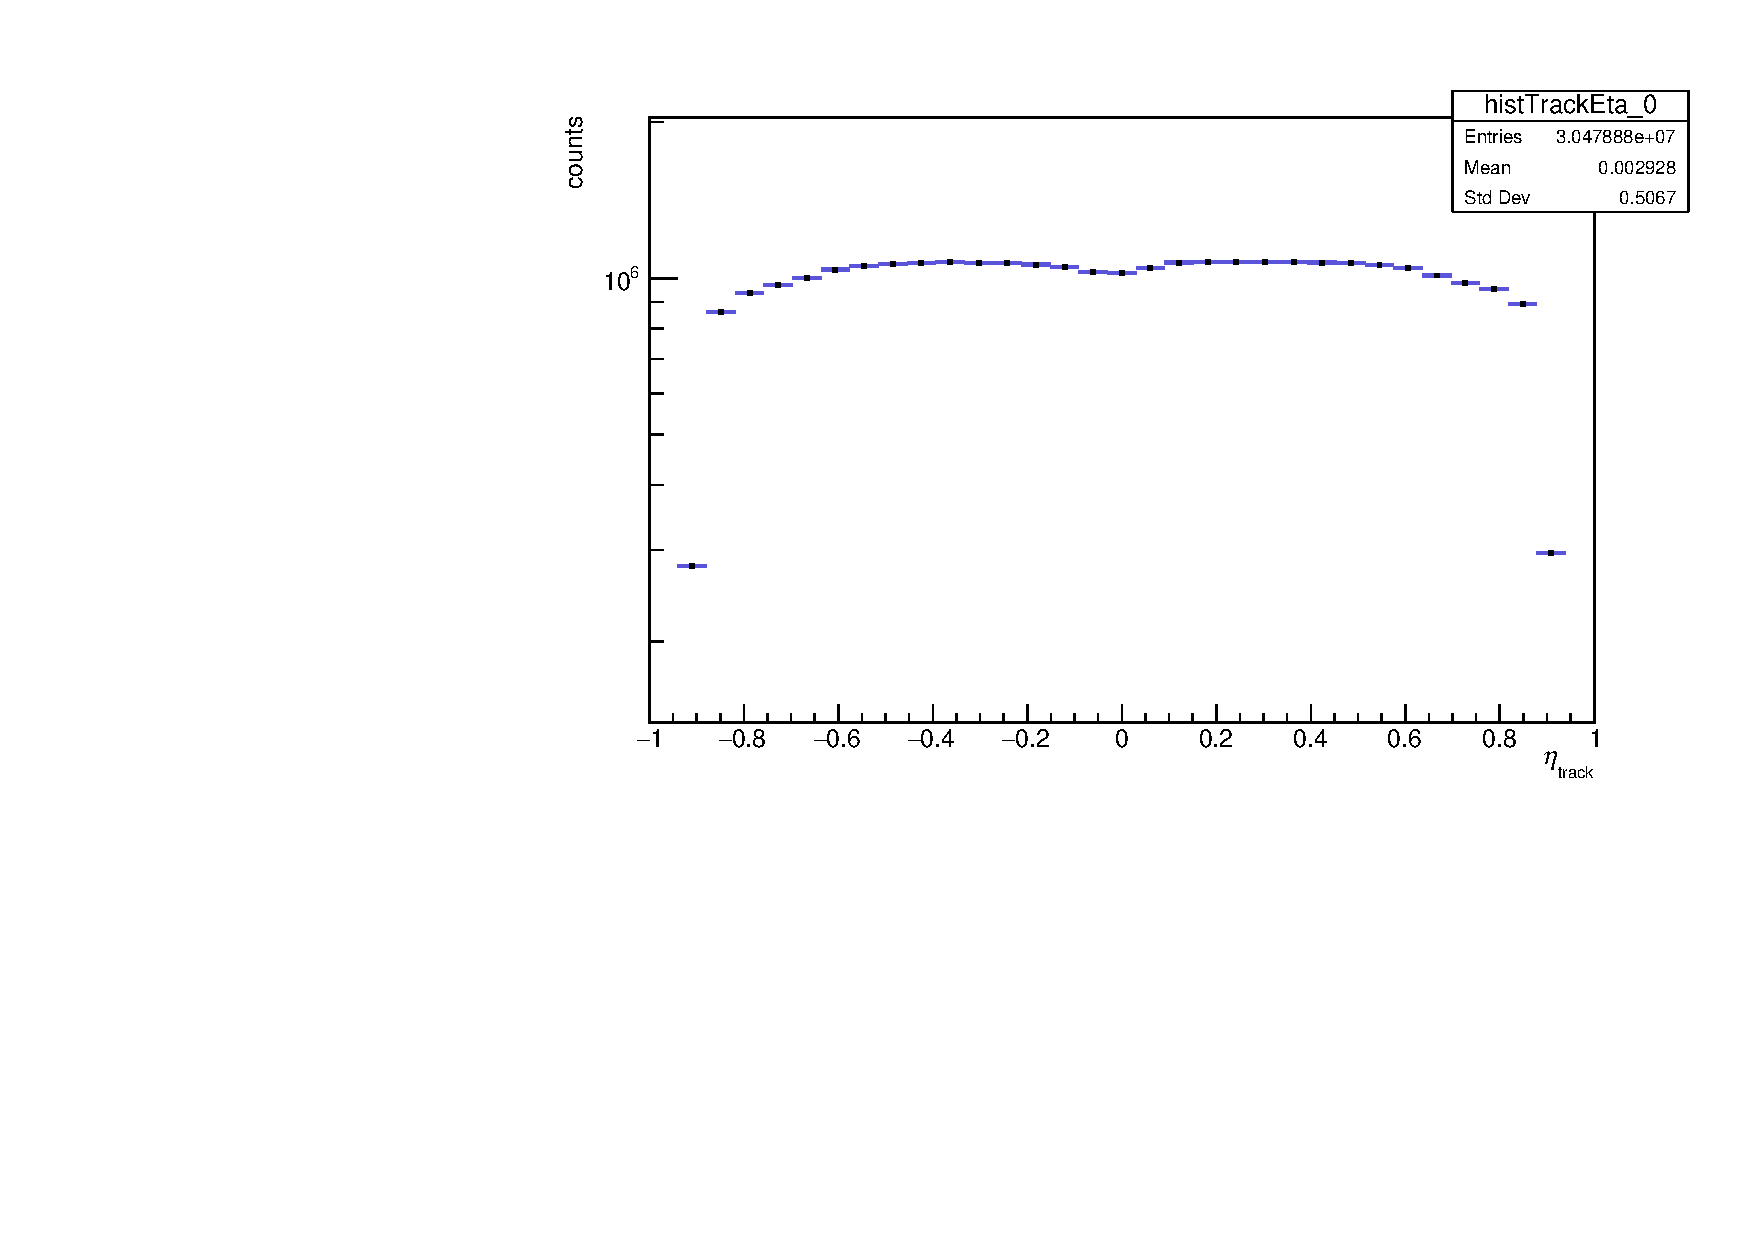
\includegraphics[width=0.4\textwidth]{tracketa} }}%
    \qquad
    \subfloat[Hybrid Track $\phi$]{{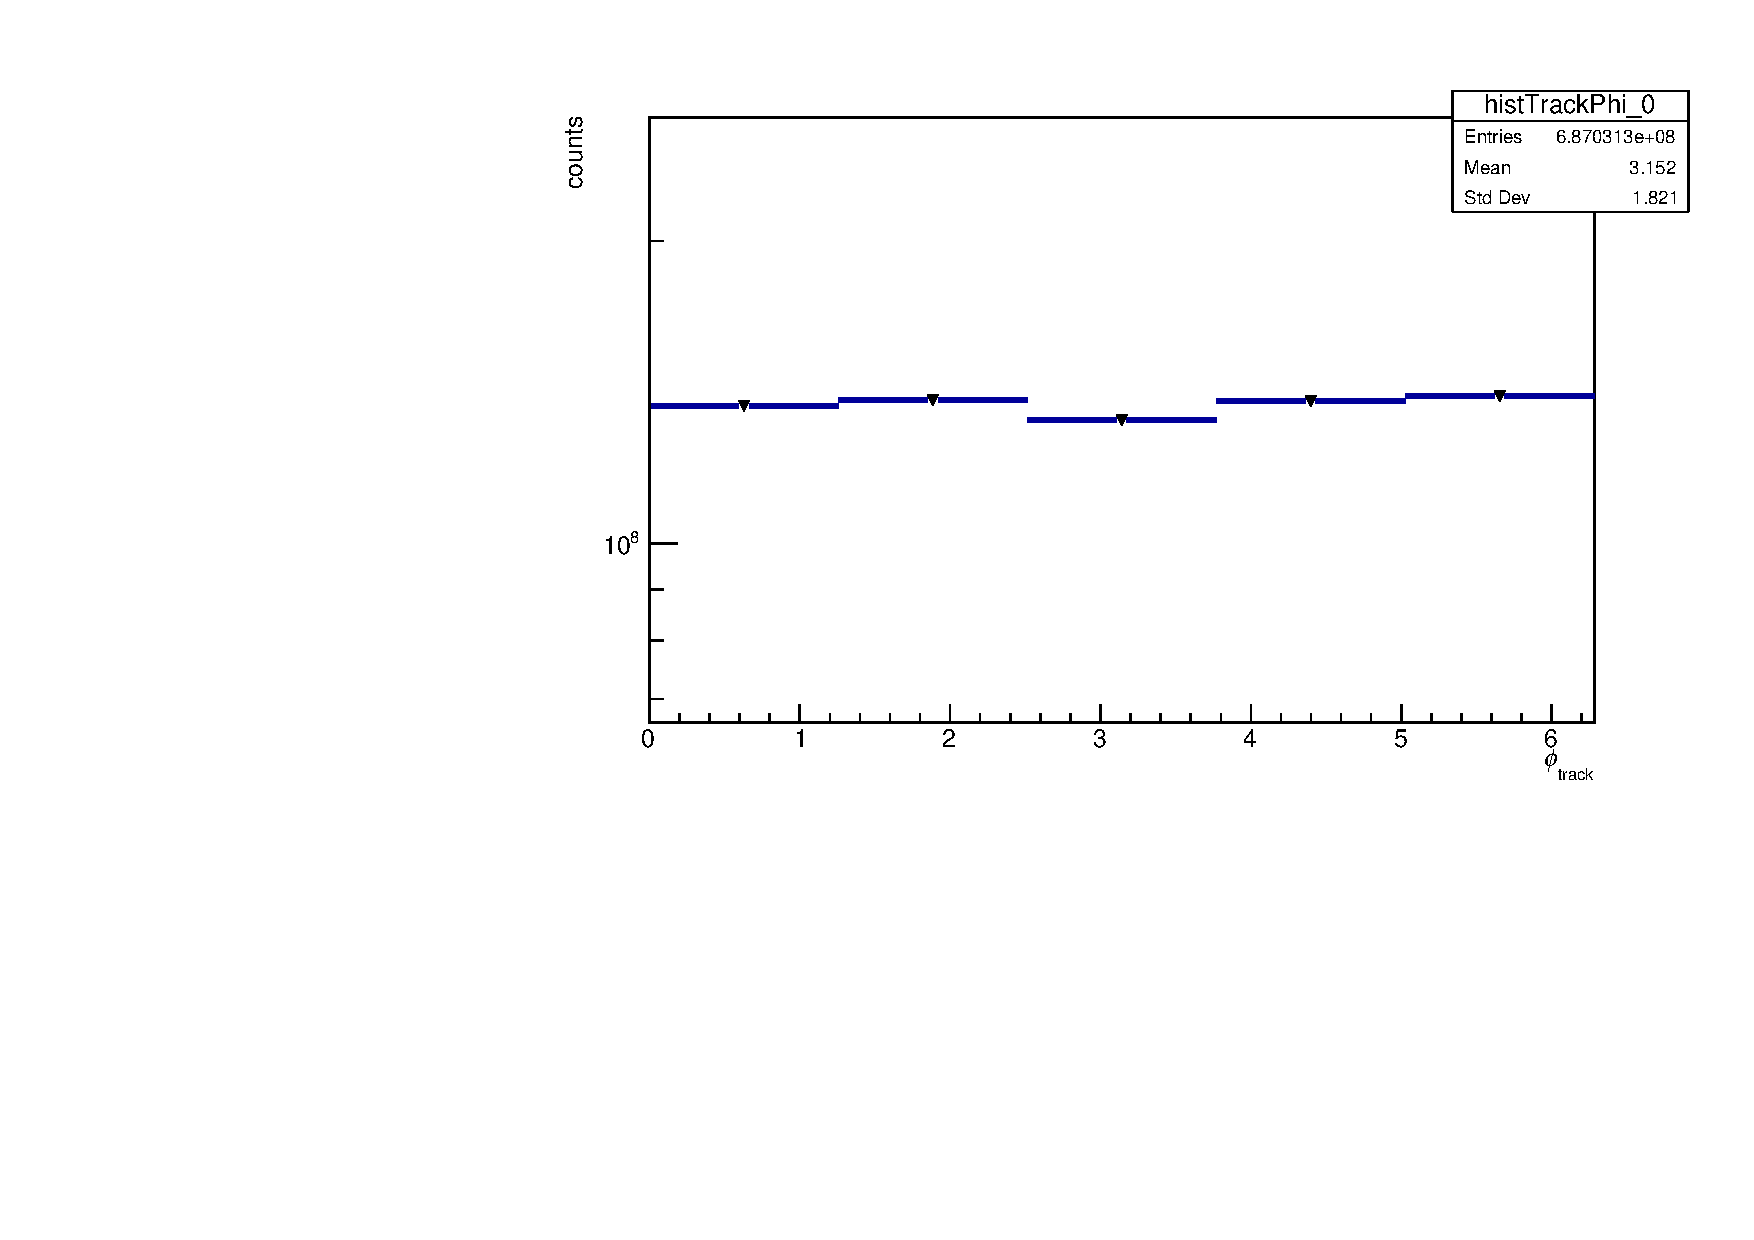
\includegraphics[width=0.4\textwidth]{trackphi} }}%
    \caption{Hybrid Track $\eta$ and $\phi$ yields.}%
    \label{fig:Hybridtracketaphi}%
\end{figure}


The quality of the jet $p_{T}$ resolution was maintained by only accepting jets into the jet finder with a resolution below 1\% as seen in Figure \ref{fig:trackresolution}, and this $p_{T}$ distribution may be seen in Figure \ref{fig:hybtrackpt}.  Tracks should travel in a smooth curve unless they decay in the detector.  Some tracks in the TPC exhibit a kink due to the particle decaying.  Due to complications that would arise from trying to include these tracks in jet finding, any track with a kink was excluded from this analysis.  These cuts followed a number of previous track cuts seen in a number of jet results published from ALICE\cite{Acharya:2018eat}.

\begin{figure}[h]
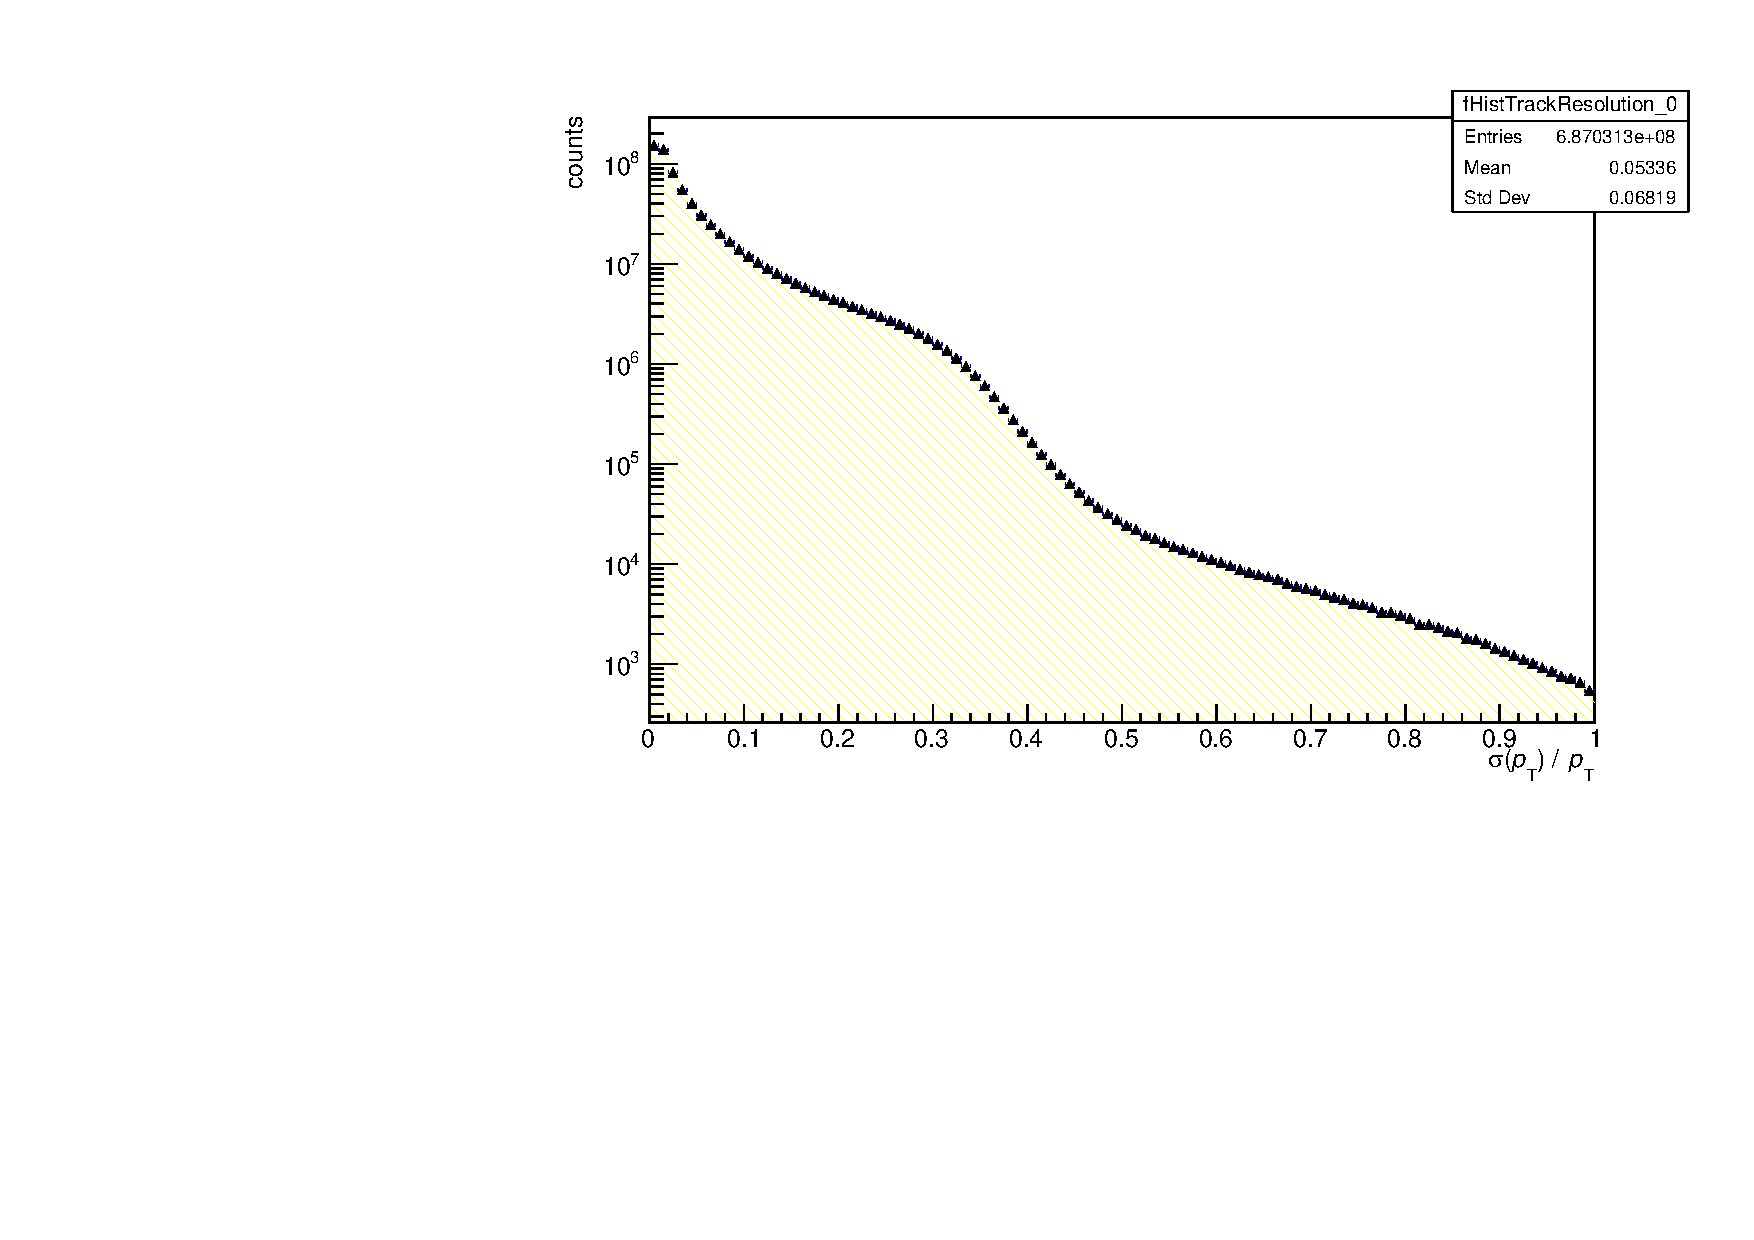
\includegraphics[width=8cm]{trackresolution}
\centering
\caption{Accepted hybrid track resolution.}
\label{fig:trackresolution}
\end{figure}

\begin{figure}[h]
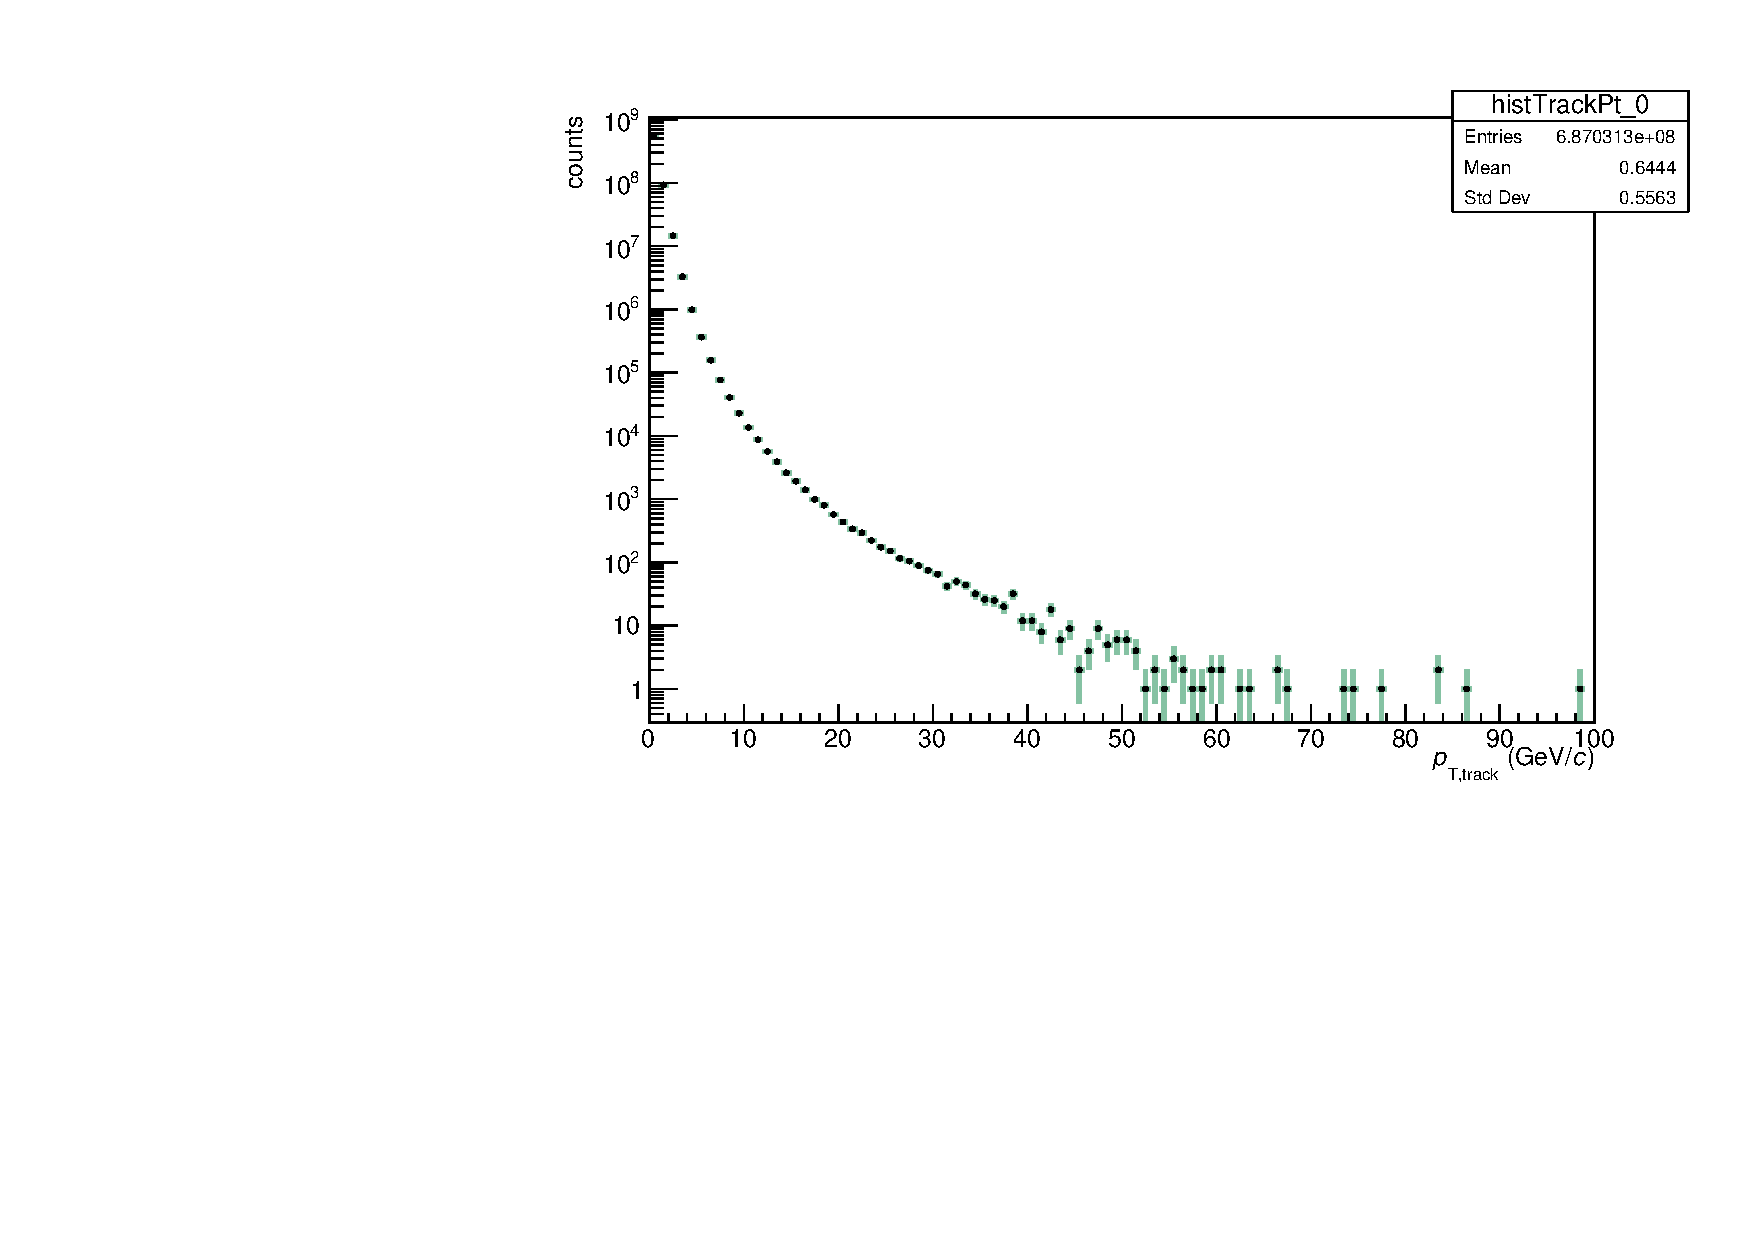
\includegraphics[width=8cm]{trackpt}
\centering
\caption{Accepted track $p_{T}$ yield.}
\label{fig:hybtrackpt}
\end{figure}


\section{Jet Selection}

Accepted tracks and clusters were pipped into the anti-kt jet reconstruction algorithm to measure inclusive jets.  A minimum threshold of 5 GeV was used to reconstruct a jet in this analysis.  A high-$p_{T}$ track threshold of 100 GeV was placed on the reconstructed jets.  This was motivated by the degradation of the momentum resolution above that energy range.  In addition a cut was applied that a jet must be composed of at least one constituent, as shown in Figure \ref{fig:JetPt} and \ref{fig:JetConst}.

\begin{figure}[h]
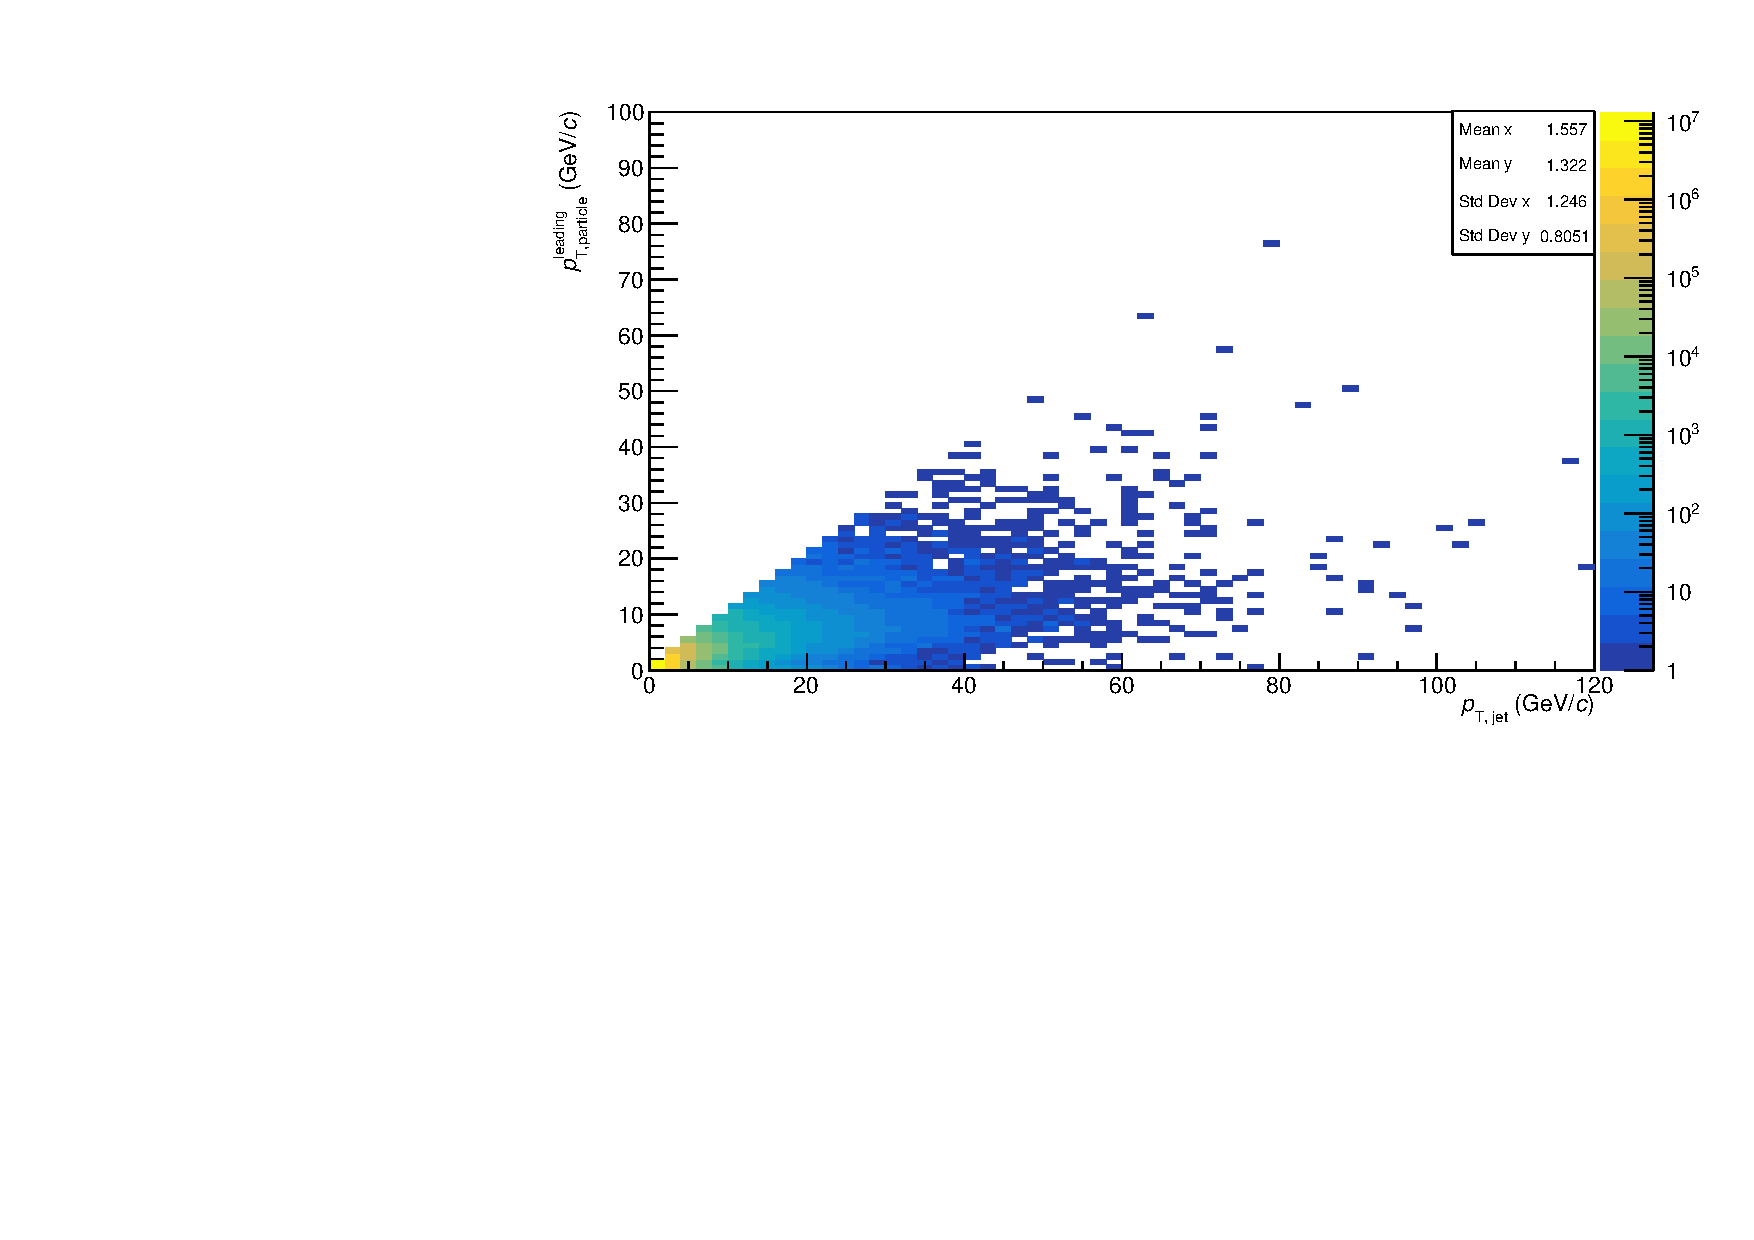
\includegraphics[width=8cm]{ptleadingR02}
\centering
\caption{R = 0.2 leading track $p_{T}$ per jet $p_{T}$.}
\label{fig:JetPt}
\end{figure}

\begin{figure}[h]
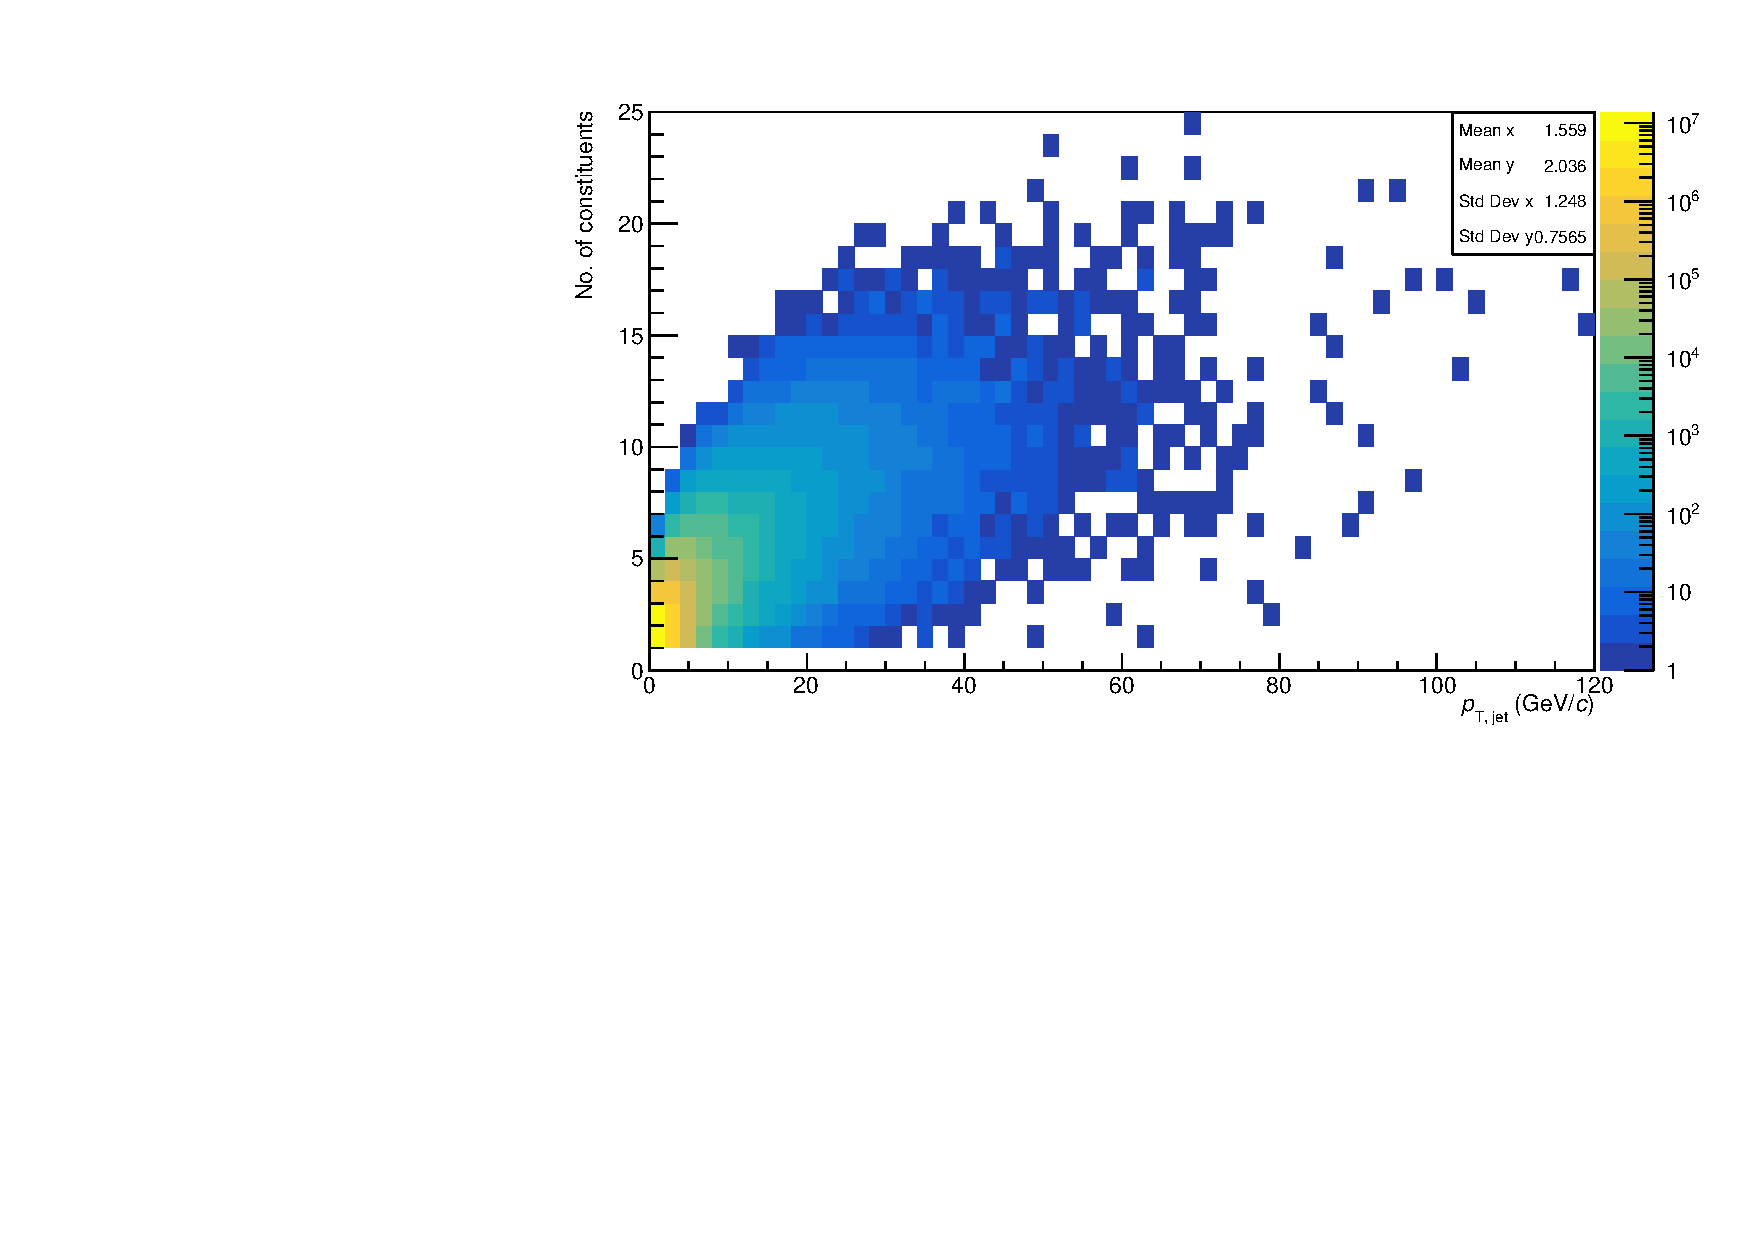
\includegraphics[width=8cm]{JetnumcconstR02}
\centering
\caption{R = 0.2 number of constituents in a jet per jet $p_{T}$.}
\label{fig:JetConst}
\end{figure}



The fragmentation function for the leading track in a jet,

\begin{equation}
z_{leading} = \frac{ p_{leading, proj} }{ p_{jet} },
\label{eq:zleading}
\end{equation}

\noindent
may be artificially high due to misidentifying secondary decay particles as primary vertex tracks and assigning them a much larger $p_{T}$.  Additionally, fake clusters, such as exotics, may skew the jet $p_{T}$ to apparently large values and thus make $z_{leading}$ infinitesimal.  

\begin{figure}[h]
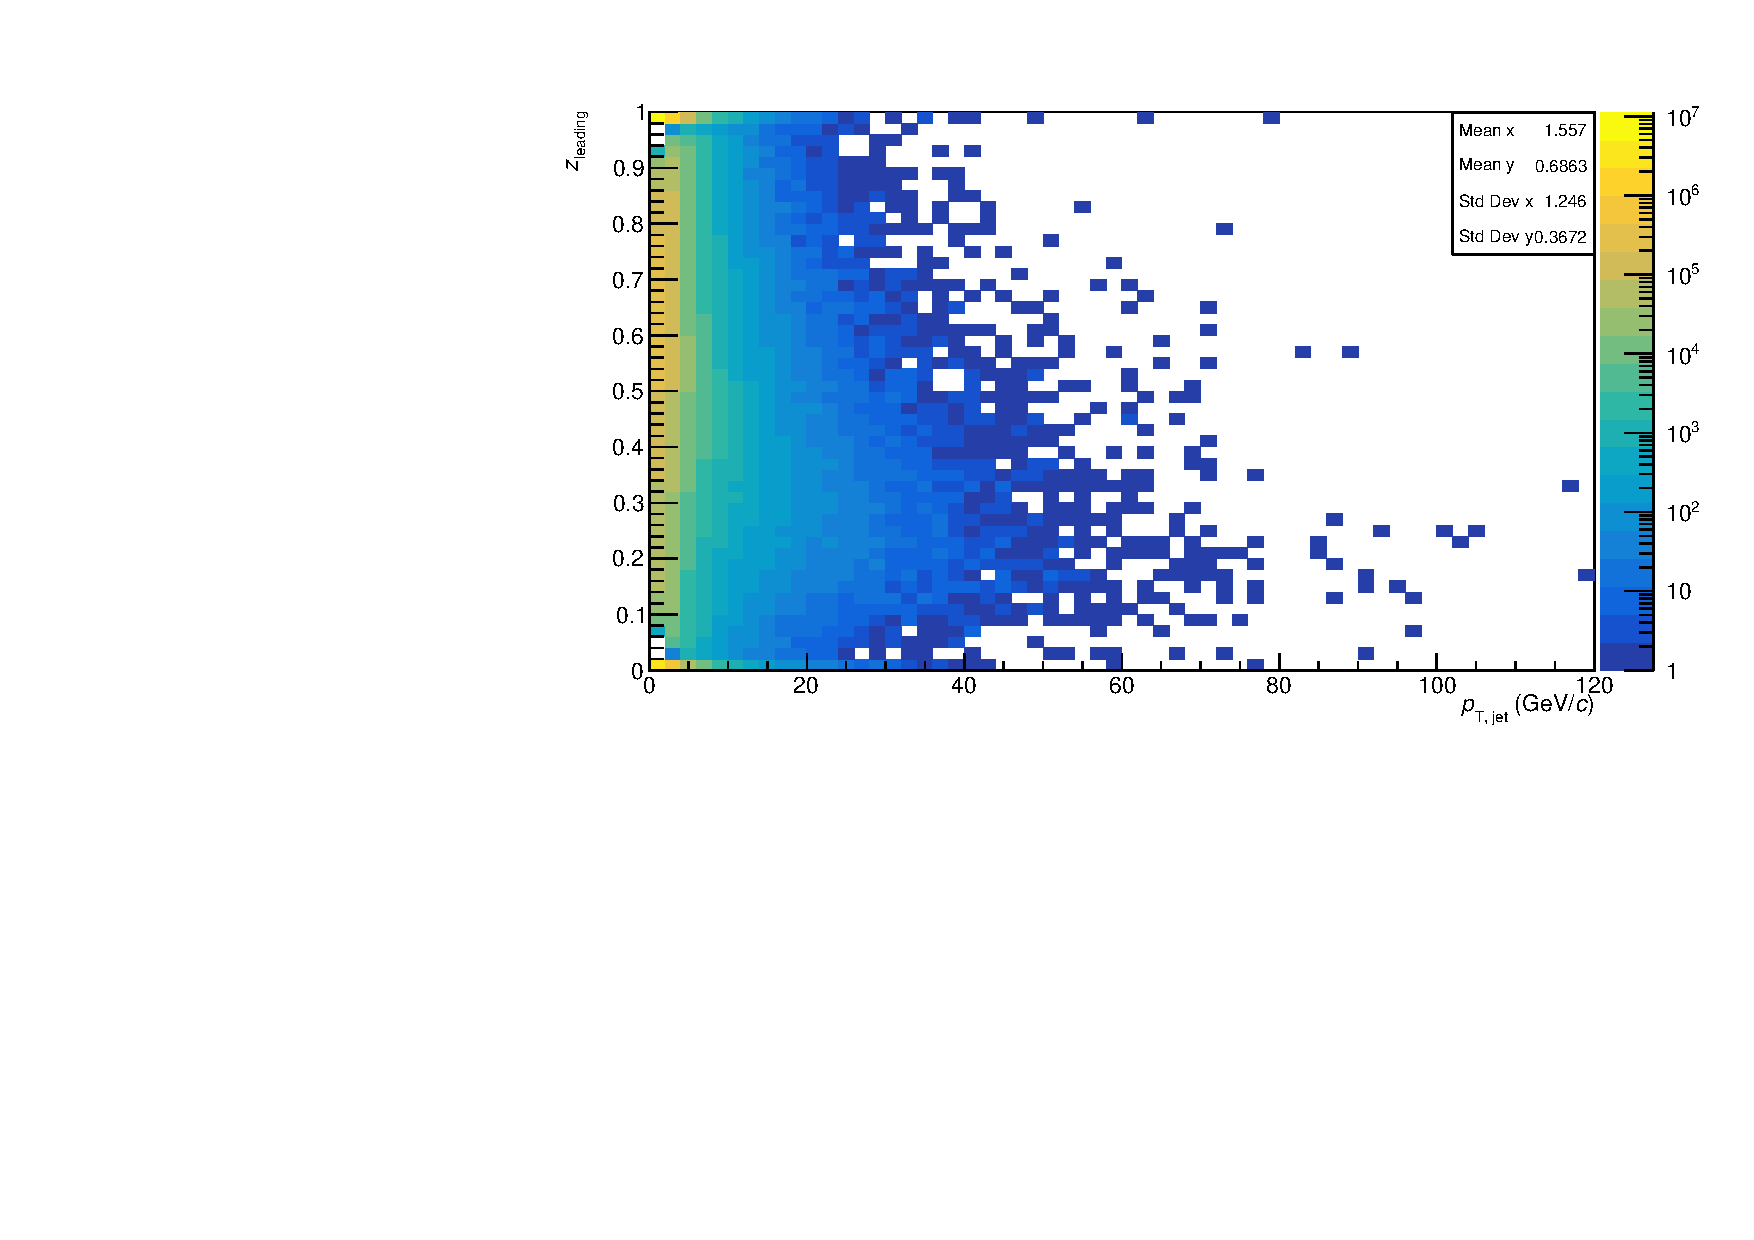
\includegraphics[width=10cm]{JetzR02}
\centering
\caption{R = 0.2 $z_{leading}$ from the Min Bias data sample.}
\label{fig:Jetz}
\end{figure}

Figure \ref{fig:Jetz} shows the projection of the hadronic 3-momentum onto the jet axis.  We observed an excess of jets, especially at low jet $p_{T}$, of z values close to 1 or zero.  Previous jet results from ALICE removed these biased jets with a cut on $ z_{leading} \geq 0.03$ and $z_{leading} \leq 0.97$ is imposed.  It should also be noted that due to QCD hadronization $z_{leading} \sim 1$ corresponds to a jet dominated by a singular high-$p_{T}$ particle, howver this is allowed by QCD and thus no $z_{leading}$ cut was implemented in this analysis.  In between .03 and .97 we see the $z_{leading}$ is continuous and uniform as expected.  

A jet area of, $A_{jet}$, cut was imposed on accepted jets.

\begin{equation}
A_{jet} \geq 0.6 \pi R_{jet}^{2}
\label{eq:AreaJet}
\end{equation}

The area is estimated in FastJet using `ghost' particles.  As jet reconstruction is being performed, these fake particles with infinitesimal $p_{T}$ are placed randomly throughout the event.  The number of ghost particles captured in a jet is proportional to the jet area, thus the precision of the jet area is sensative to the reconstruction of soft particles.  Figure \ref{fig:jetRejection} shows the rejection reason for a jet with the dominate reasoning due to the area cut, this cut skewed towards low-$p{T}$ jets.

\begin{figure}[h]
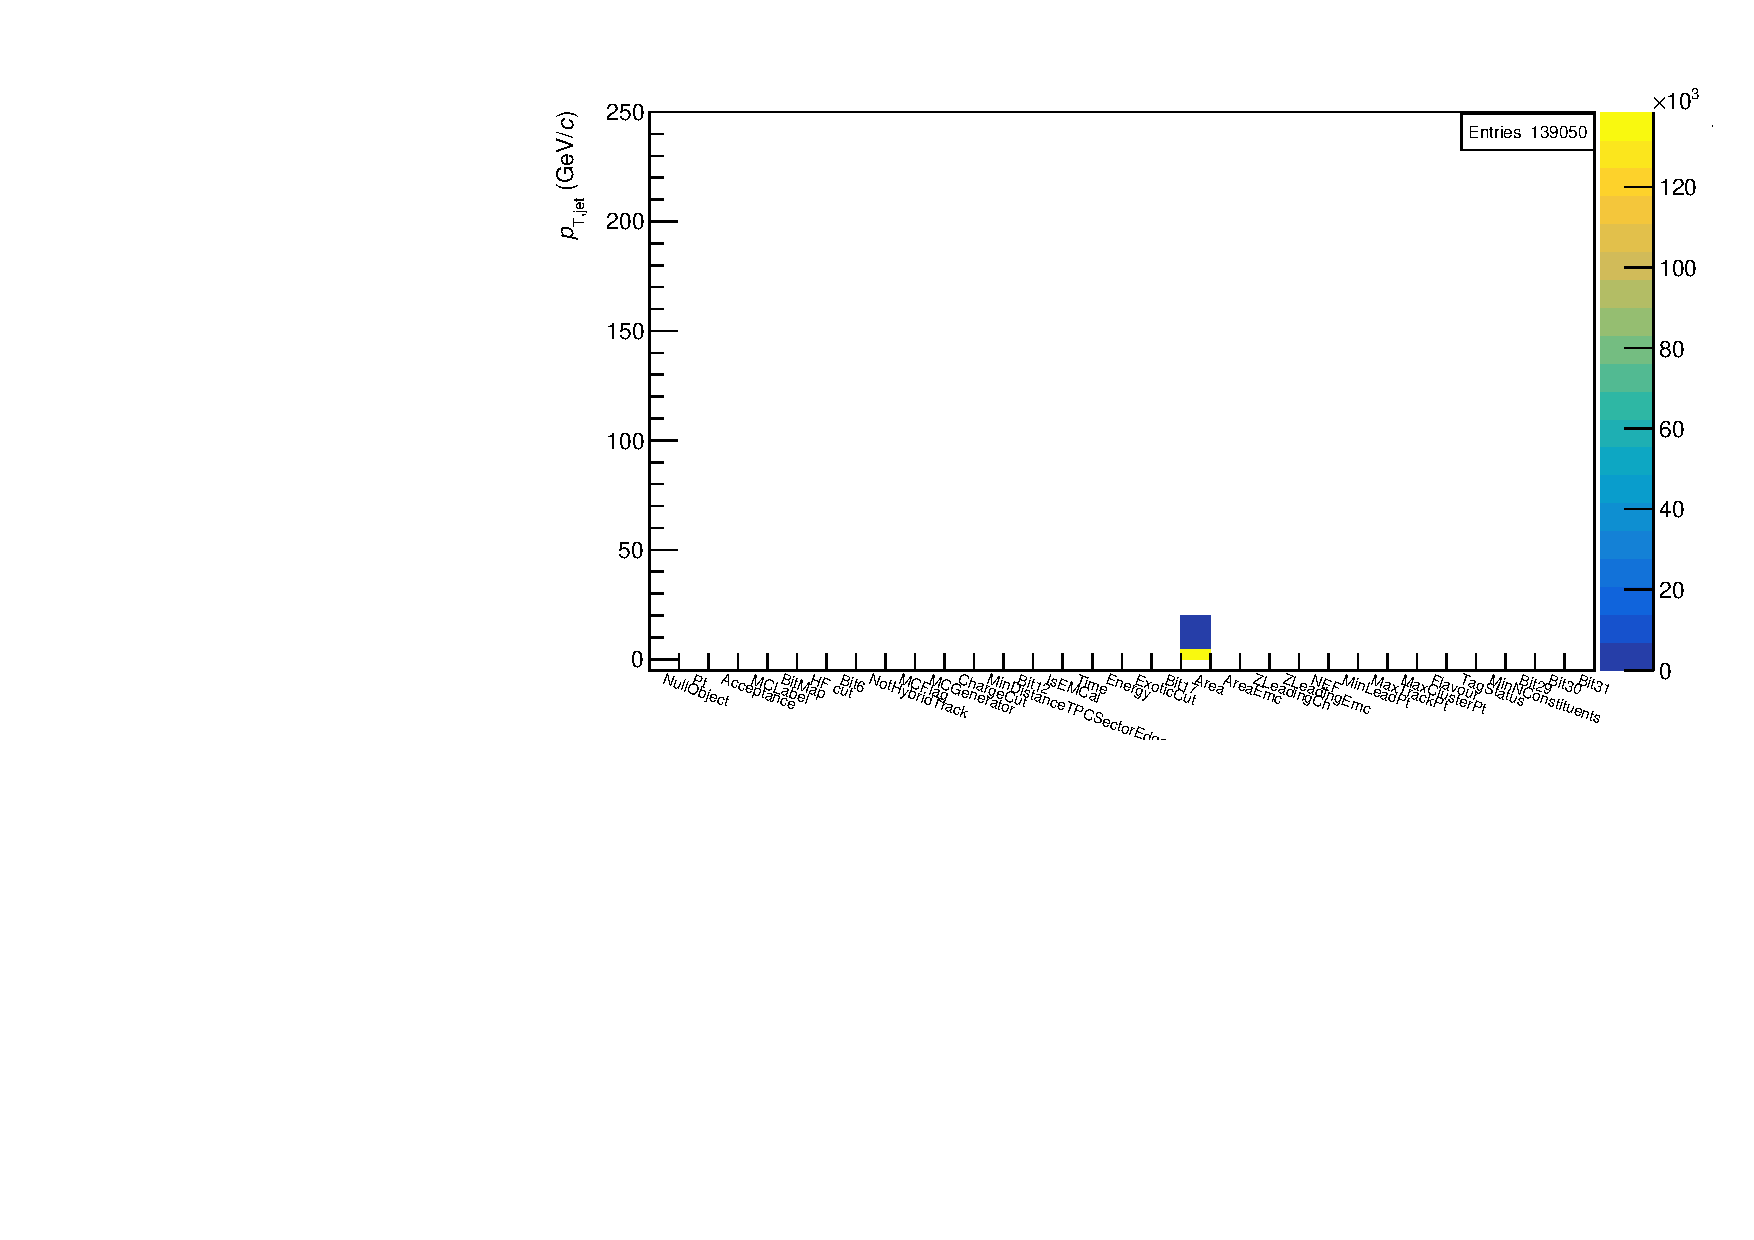
\includegraphics[width=12cm]{jetRejection}
\centering
\caption{Jet rejection reason.}
\label{fig:jetRejection}
\end{figure}


The Neutral Energy Fraction (NEF) is the total jet energy carried by the neutral components of the jet, i.e. EMCal clusters.  Figure \ref{fig:JetNEF} shows the NEF for R = 0.2 jets from the Min Bias sample.


We observed an excess of jets at low-$p_{T}$ with NEF values around zero or one, similar to what was seen with the $z_{leading}$ distribution.  The cause for these excesses were explored in this analysis, but no hard source was identified and no cut to the NEF was used.  Because this is not a well understood pheonmena no NEF cut was implemented, but this is something that should be explored in future analysis.


After this exploratory data analysis was performed and the cuts that were used were implemented I obtained my sample of the signal jets that are reported in the cross section and spectra.  These criteria were implemented for the R = 0.3 and R = 0.4 along with the EMCal triggered data.

\begin{figure}[h]
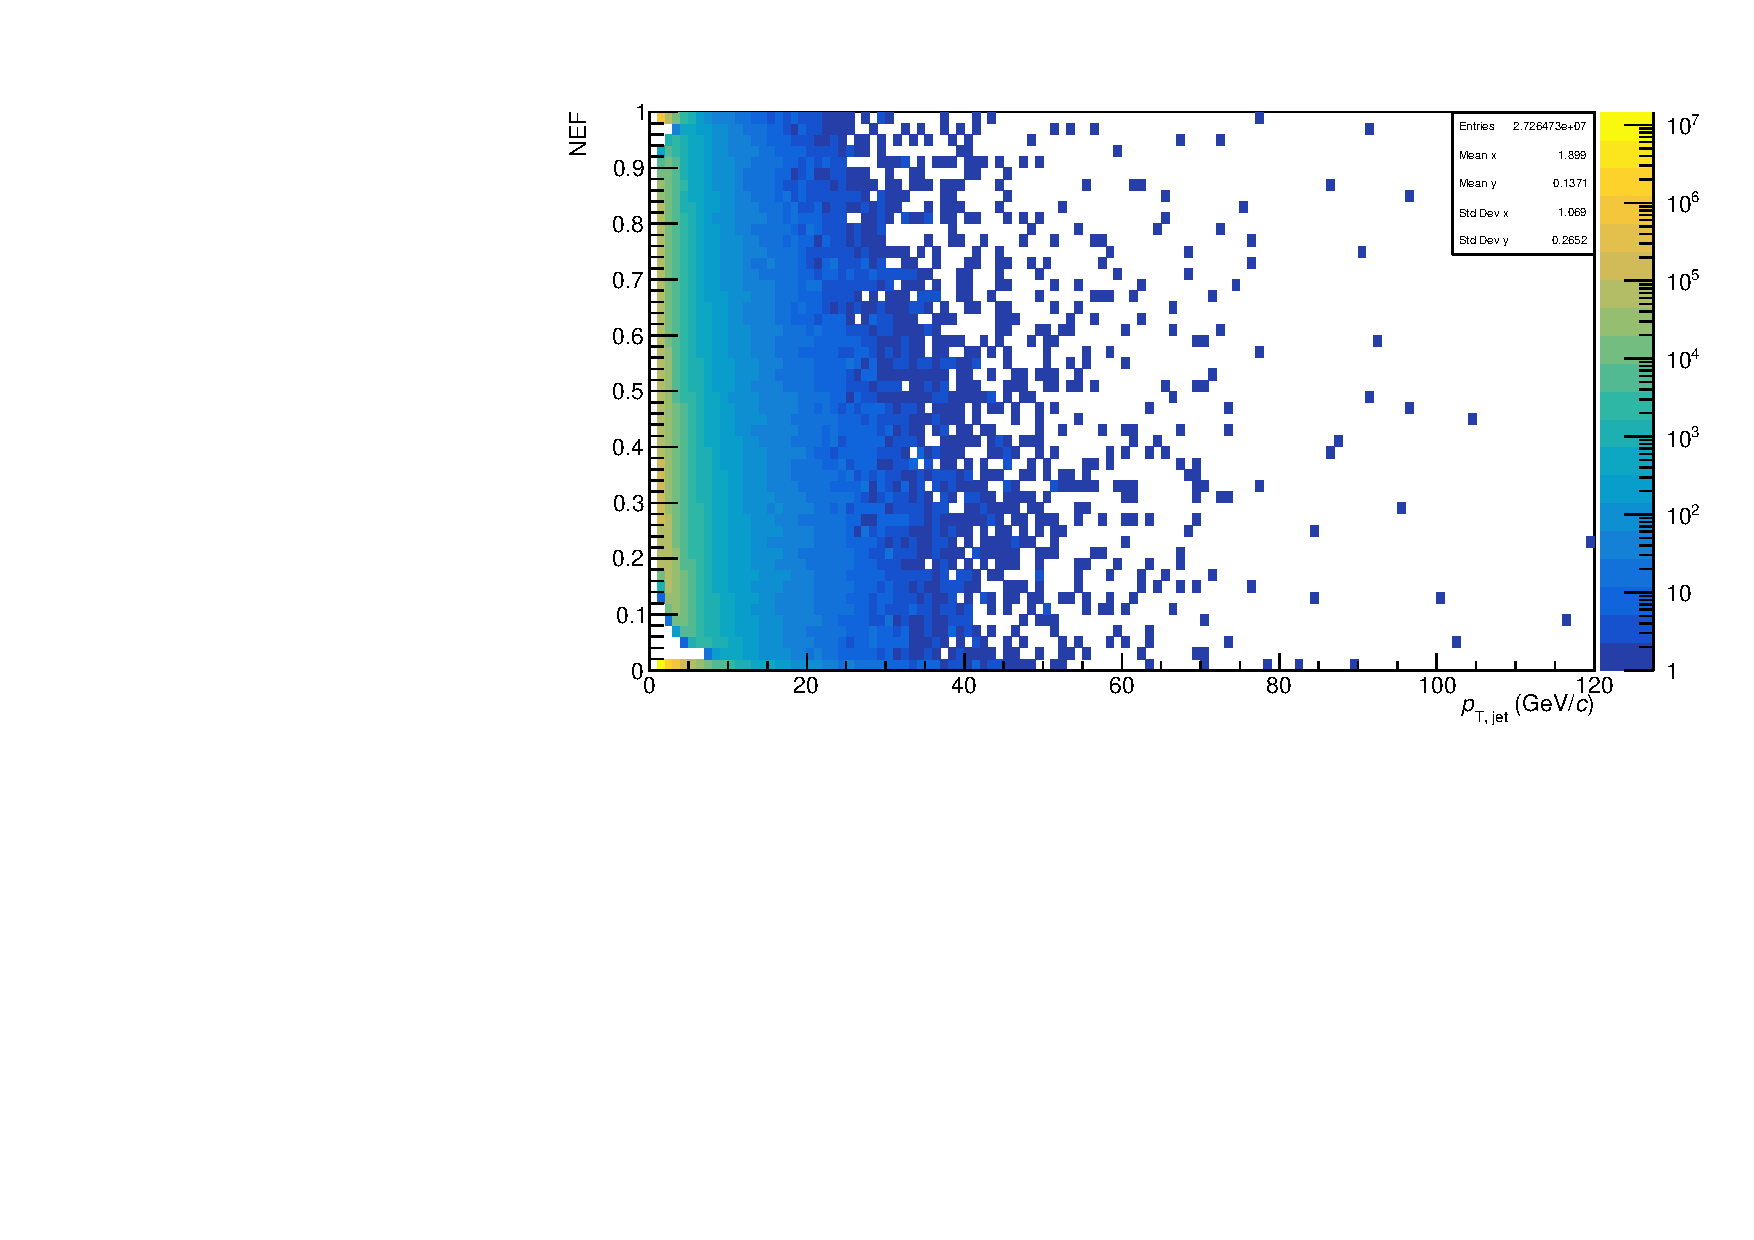
\includegraphics[width=10cm]{NEFR02}
\centering
\caption{R = 0.2 NEF per jet $P_{T}$.}
\label{fig:JetNEF}
\end{figure}


\section{Acceptance Correction}
Jet spectra, cross-sections, and ratios of cross-sections are reported over the full azimuth angle and psuedorapidity acceptance in this thesis.  However, due to jets being constrained to the EMCal, a geometric factor was used to correct for the limited acceptance of the detector.  This thesis explored jet radii between 0.1 and 0.5, in order to study the effects of wide angle radiation on jet fragmentation.  Jet measurements in heavy-ion collisions use radii, typically of 0.2, to help negate the high multiplicity background.  Due to these geometric corrections the centroid of a jet is constrained to,

\begin{equation}
|\eta_{jet}| \leq 0.7 - R, \; 1.4 + R \leq \phi_{jet} \leq 3.14 -R.
\label{eq:jetconstration}
\end{equation}

\begin{equation}
A(p_{T}) = \frac{(1.4 - 2R) \times (1.745 - 2R)}{2 \pi}.
\label{eq:acceptance}
\end{equation}

For jets between R = 0.1 through R = 0.5 the following jet acceptance corrections were used, see Table 5.2.

\begin{table}[hb]
\label{tab:AcceptanceFactor}
\begin{center}
\begin{tabular}[b]{|c|c|c|}
	\hline
	Jet R & $A(p_{T})$ \\ \hline
	0.1 & 0.296 \\ \hline
	0.2 & 0.214\\ \hline
	0.3 & 0.146\\ \hline
	0.4 & 0.091\\ \hline
	0.5 & 0.048\\ \hline
\end{tabular}
\end{center}
\caption{EMCal jet acceptance for radii 0.1 - 0.5.}
\end{table}



\section{Corrections to Monte Carlo}

The reconstructed jet $p_{T}$ has a number of detector effects `folded' into the measurement.  These effects included such things as:

\begin{itemize}
\item Tracking inefficiencies from the TPC and ITS.
\item Missing jet energy components from long-lived particles, such as the $K^{0}_{L}$ and neutron, that are cut by the EMCal timing requirement.
\item TPC track $p_{T}$ and EMCal cluster energy resolutions.
\item Hadronic corrections to the EMCal cluster spectrum.
\item Material loss in the detectors.
\end{itemize}

\noindent
Unfolding is a method by which these detector effects are removed from the raw inclusive jet spectra so that a `true' jet spectra may be obtained and compared with theoretical calculations or other experimental results.  

In order to unfold a jet spectra, it is necessary to generate a response matrix that simulates the described effects above.  After the response matrix is generated a number of statistical approaches including, Bayesian, Singular Value Decomposition (SVD), or Bin-by-Bin, may be applied to unfold the raw jet spectra.  In order to generate the response matrix, a Pythia generated event is embedded into a GEANT simulation of the ALICE detector.  Due to the fact that the performance and efficiency of the ALICE detector may change between the data taking periods each simulation is `anchored' to a given LHC.  These anchors contain all the hot and dead sectors for the subdetectors, along with their calibrated performance during that specified data taking.  Two Monte Carlo data sets were produced with the Min Bias trigger simulated for the full 8 TeV run, the first was a Pythia generator using the Monesh-2013 tune and the second was a Min Bias tune of the PHOjet Monte Carlo package.  Both data sets were explored for this thesis and it was decided that the final corrected spectra would be obtained via unfolding with the Pythia Monte Carlo data set.  The magnitude of any one of the effects unfolding is supposed to account for is not expected to be very large, but combined may be significant, thus unfolding is an important step in this analysis.

\subsubsection{Response Matrix}
Given a truth-level, the Monte Carlo event at the particle level, jet $p_{T}$ we wish to reconstruct that jet's $p_{T}$ at the detector-level.  The particle-level Pythia jets are constructed from the primary particles generated via Pythia, while excluding any daughter decay particles in order to avoid double counting.  In addition the tracking efficiency in Pythia is known to deviate from nature.  This is due to Pythia under predicting the production of strange quarks.  
Constructing the response matrix in this case was calculated on a jet-by-jet basis.  The particle-level jet centroid ($\phi_{part}$,$\eta_{part}$)is matched to the detector-level jet via a constrain on the displaced distance between the two jet centroids in ($\phi$,$\eta$).  This distance was constrained to: $\Delta  R = \sqrt{(\phi_{part} - \phi_{det})^{2} + (\eta_{part} - \eta_{det})^{2}} \leq 0.25 \; $.  Once a jet was matched at the detector level to a jet generated from the particle level the response matrix was incremented by jet $p_{T}$ at both the detector and Monte Carlo levels.  The response matrix was generated with a fine binning width of 1 GeV. 

\begin{figure*}[t!]
$\begin{array}{rl}
    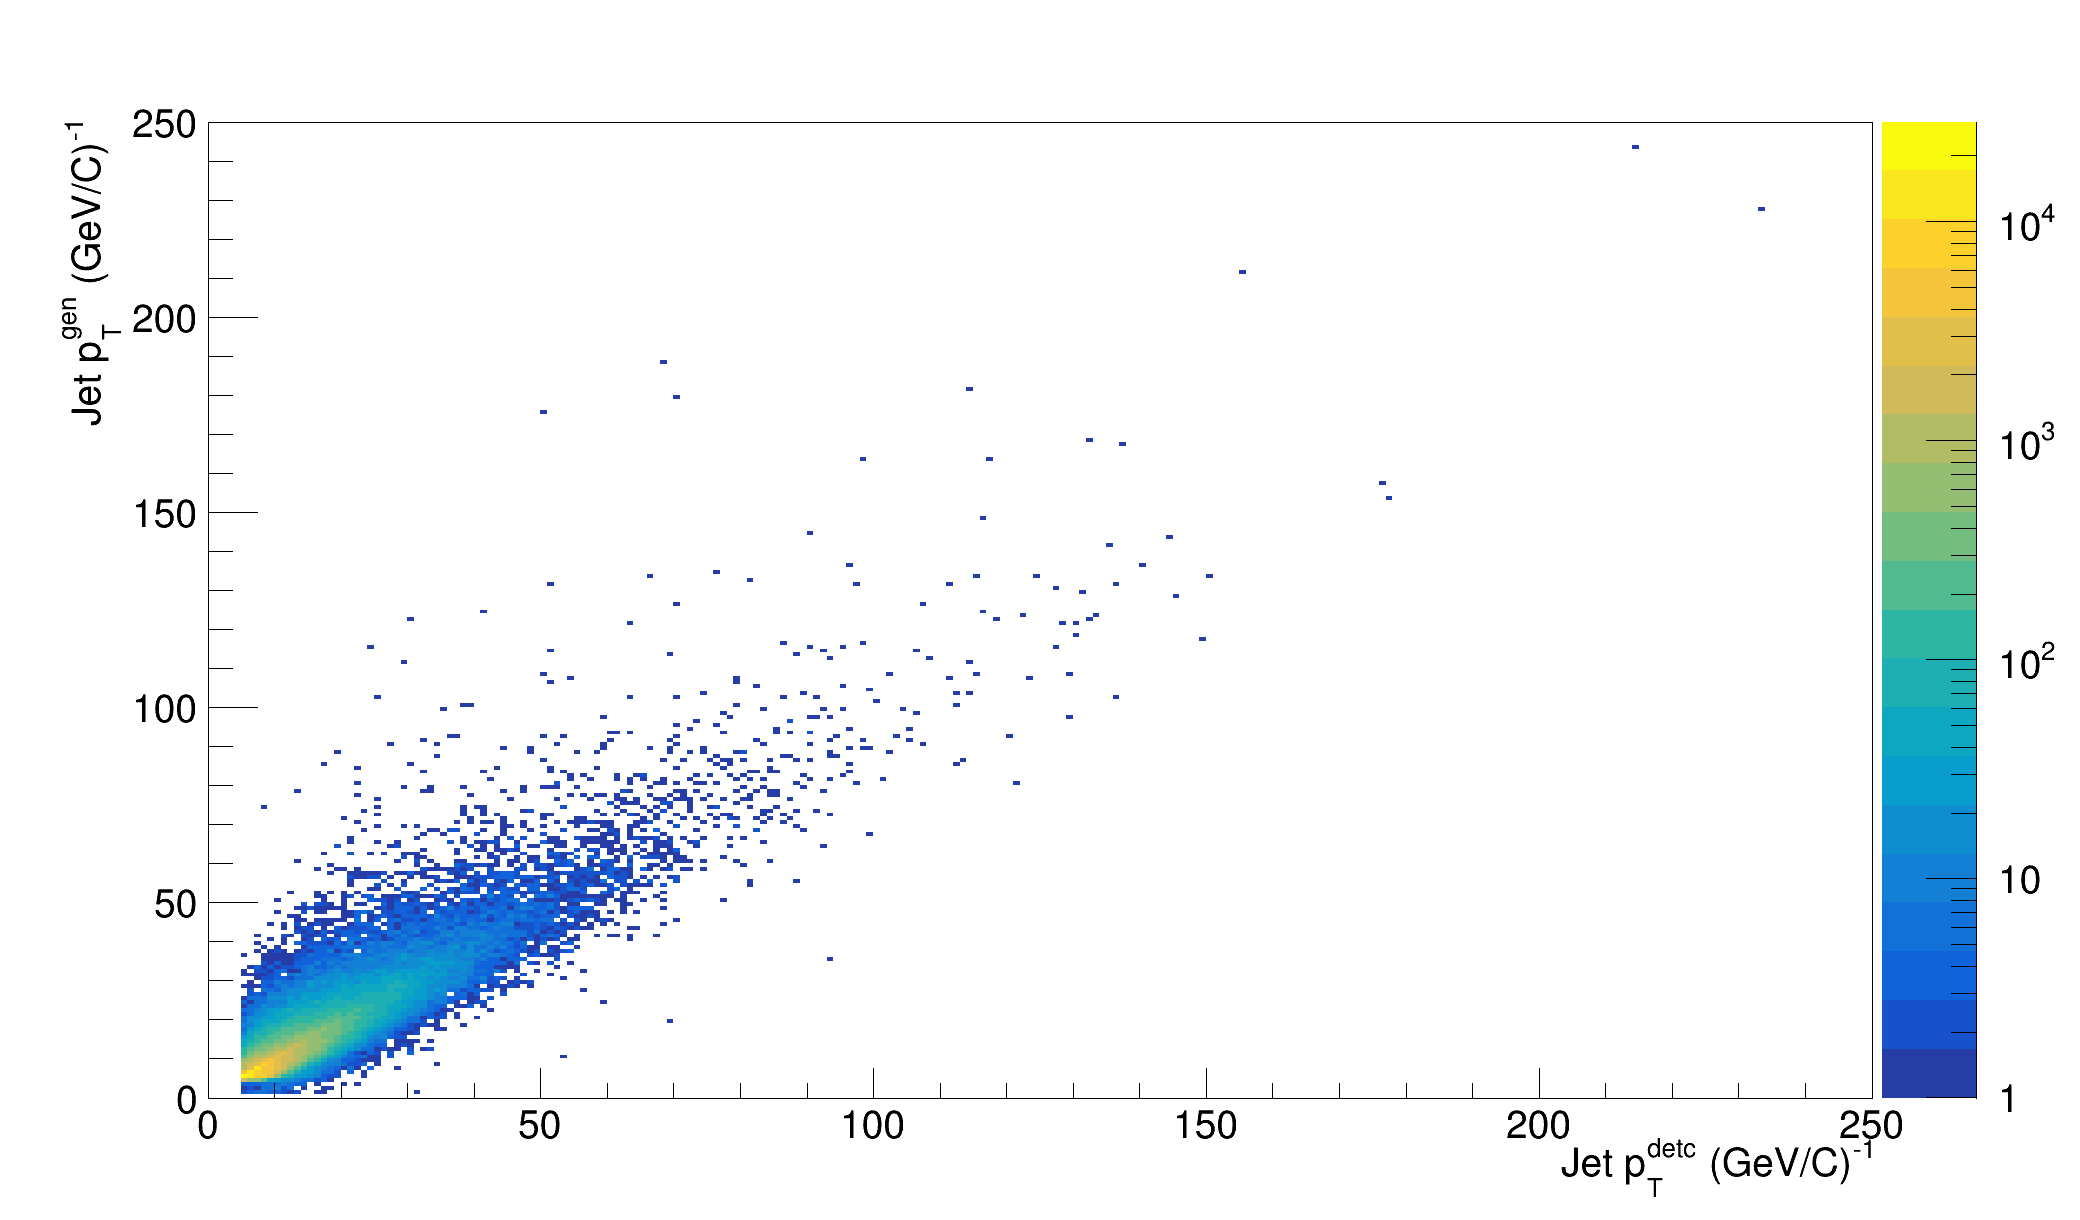
\includegraphics[width=0.5\textwidth]{responseR02} &
    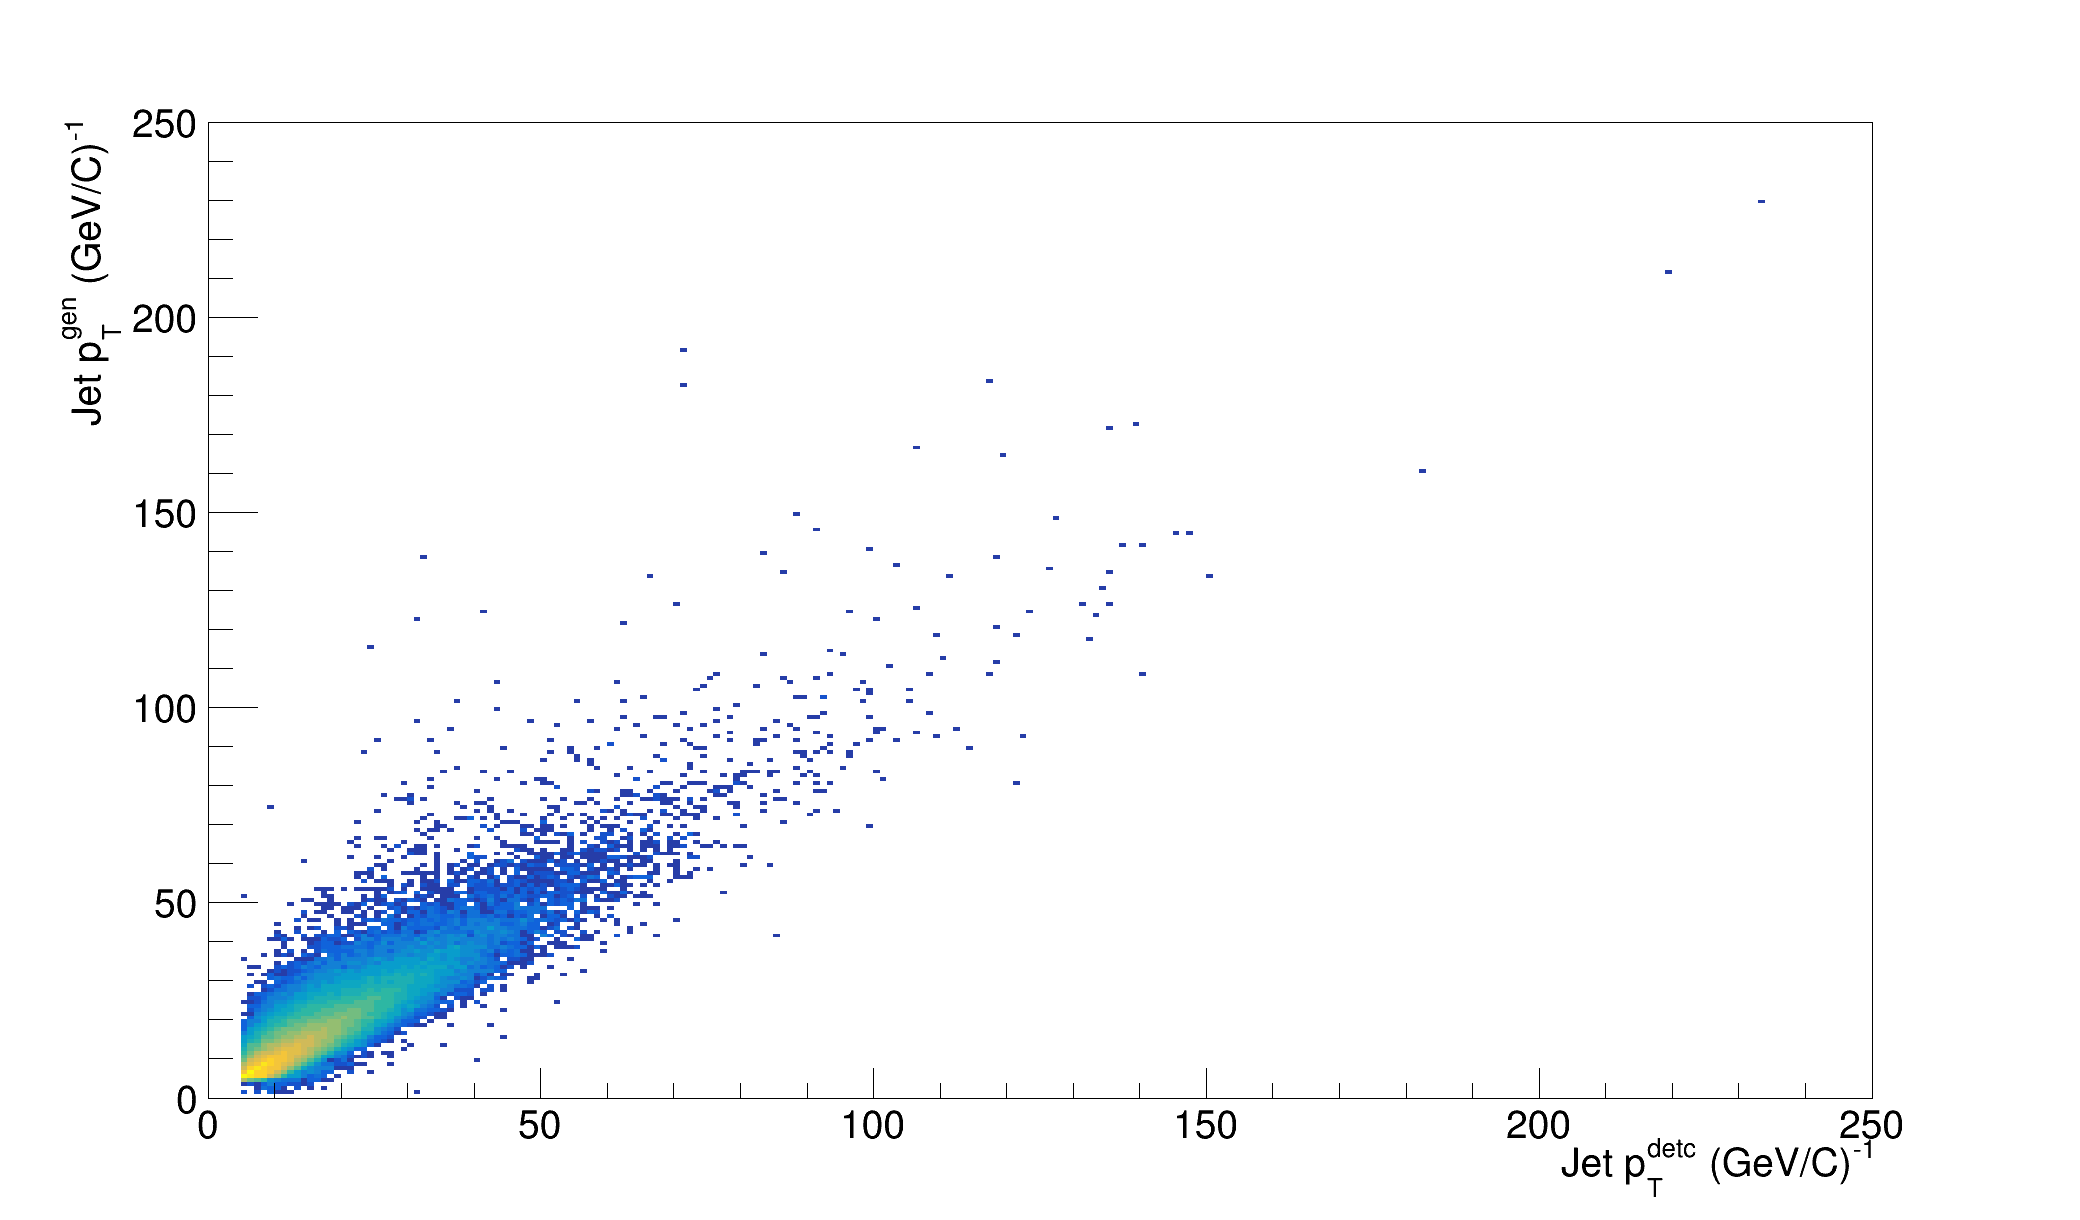
\includegraphics[width=0.5\textwidth]{responseR03}\\
    \multicolumn{2}{c}{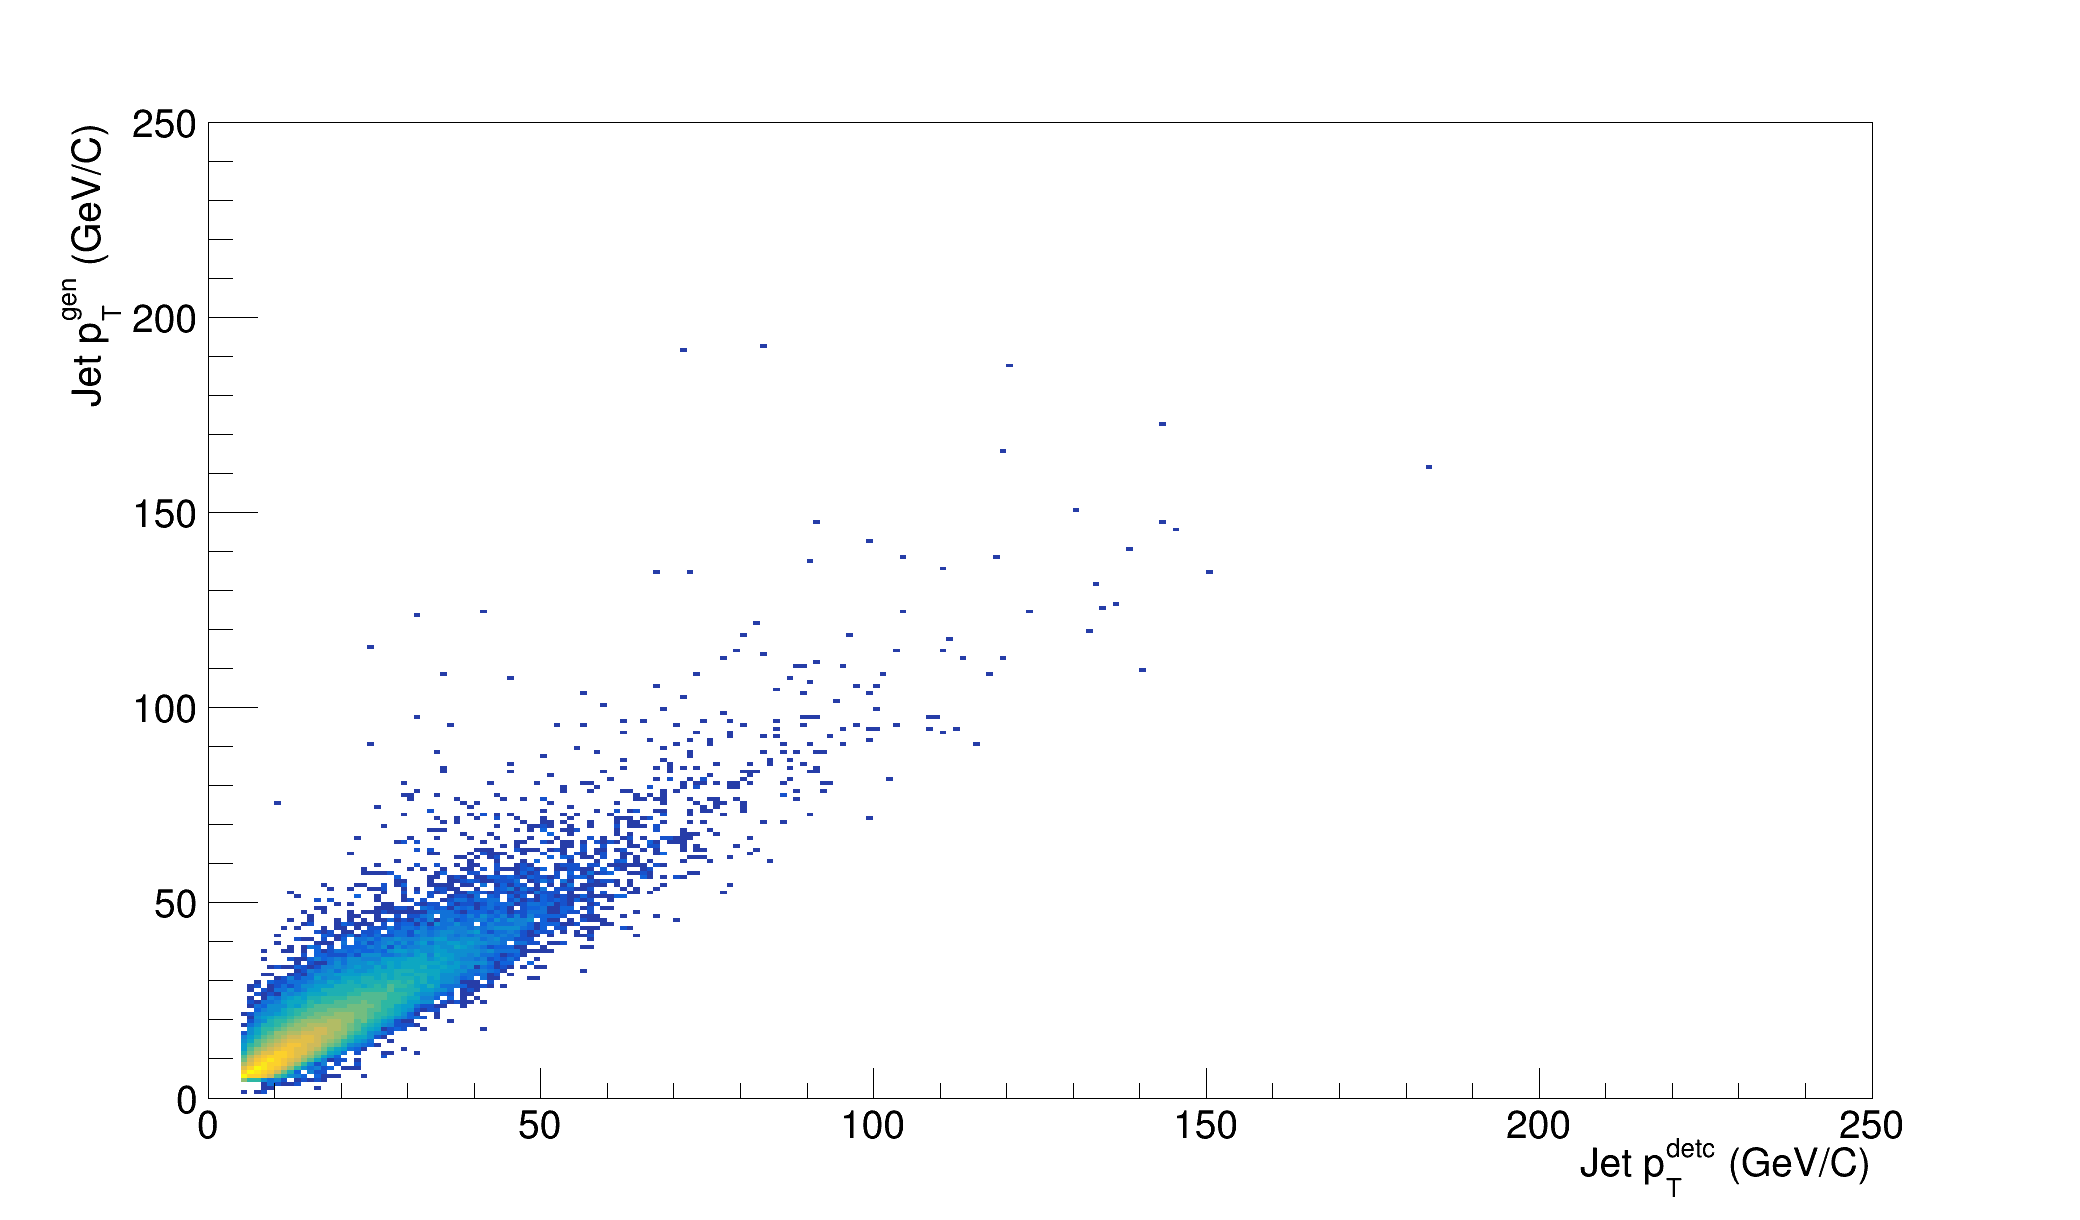
\includegraphics[width=0.5\textwidth]{responseR04}}
\end{array}$
\caption[Response Matrices for R = 0.2, R=0.3, and R = 0.4 jets.]{\label{fig:response}Response Matrices for R = 0.2, R=0.3, and R = 0.4 jets.}
\end{figure*}

Figure \ref{fig:response} shows the response matrices for the R = 0.2, R = 0.3, and R = 0.4 jets generated with the prescribed manner.  The response matrices display a linear relationship below 50 GeV on both axis and show that above $\sim$100 GeV the matrices are statistically starved.  This is primarily because the Monte Carlo Pythia and PHOJet data sets generated for the 8 TeV pp run did not model the high-$p_{T}$ triggers associated with the EMCal.  The particle jet finders configured for the response matrices allowed for jet finding down to a 100 MeV jet candidate at the particle level with no constraints on the minimum particle momentum or energy for a constituent.  The detector level jet finders were configured in the same manner as they were for the raw jet spectra measurement.  

\subsubsection{Corrections to Particle Level}

Unfolding was performed using the \verb+RooUnfold+\cite{Adye:2011gm} software package.  Corrections were applied using the bin-by-bin\cite{Cowan:2002in} algorithm. 

\begin{equation}
C_{MC} \big( p_{T}^{low} : p_{T}^{high} \big) =  \frac{  \int^{p_{T}^{high}}_{p_{T}^{low}} dp_{T} \; \frac{dF^{uncorr}_{meas}}{dp_{T}} \times \frac{d^{2}N^{particle}_{MC}/d\eta \, dp_{T}}{d^{2}N^{detector}_{MC}/d\eta \, dp_{T}}  } { \int^{p_{T}^{high}}_{p_{T}^{low}} dp_{T} \; \frac{dF^{uncorr}_{meas}}{dp_{T}} }
\label{eq:binbybin}
\end{equation}

\noindent
where $d^{2}N^{particle}_{MC}/dp_{T} \, d\eta$ is the Pythia particle level inclusive jet spectra, $d^{2}N^{detector}_{MC}/dp_{T} \, d\eta$ is the GEANT detector level inclusive jet spectra, $dF^{uncorr}_{meas} / dp_{T}$ is a weight function which minimizes the dependence on the two simulation spectra shapes, and finally $p_{T}^{low}$ and $p_{T}^{high}$ are the lower and upper bin limits.  Due to the limited statistics derived from the Monte Carlos available, the unfolding procedure was stable only in unfolding the truth level jet spectra for the range: $p_{T,jet} \, \epsilon \;$ [10 GeV, 120 GeV] for both the raw Min Bias and EMCal triggered data sets.  The only way to get around this crutch to the analysis would be to ask the ALICE collaboration to make new official particle + detector level simulations that included the EMCal trigger.  The final truth value for the jet spectra will be reported in this range.



\subsubsection{Unfolded MB Spectra}

\begin{figure}[h]
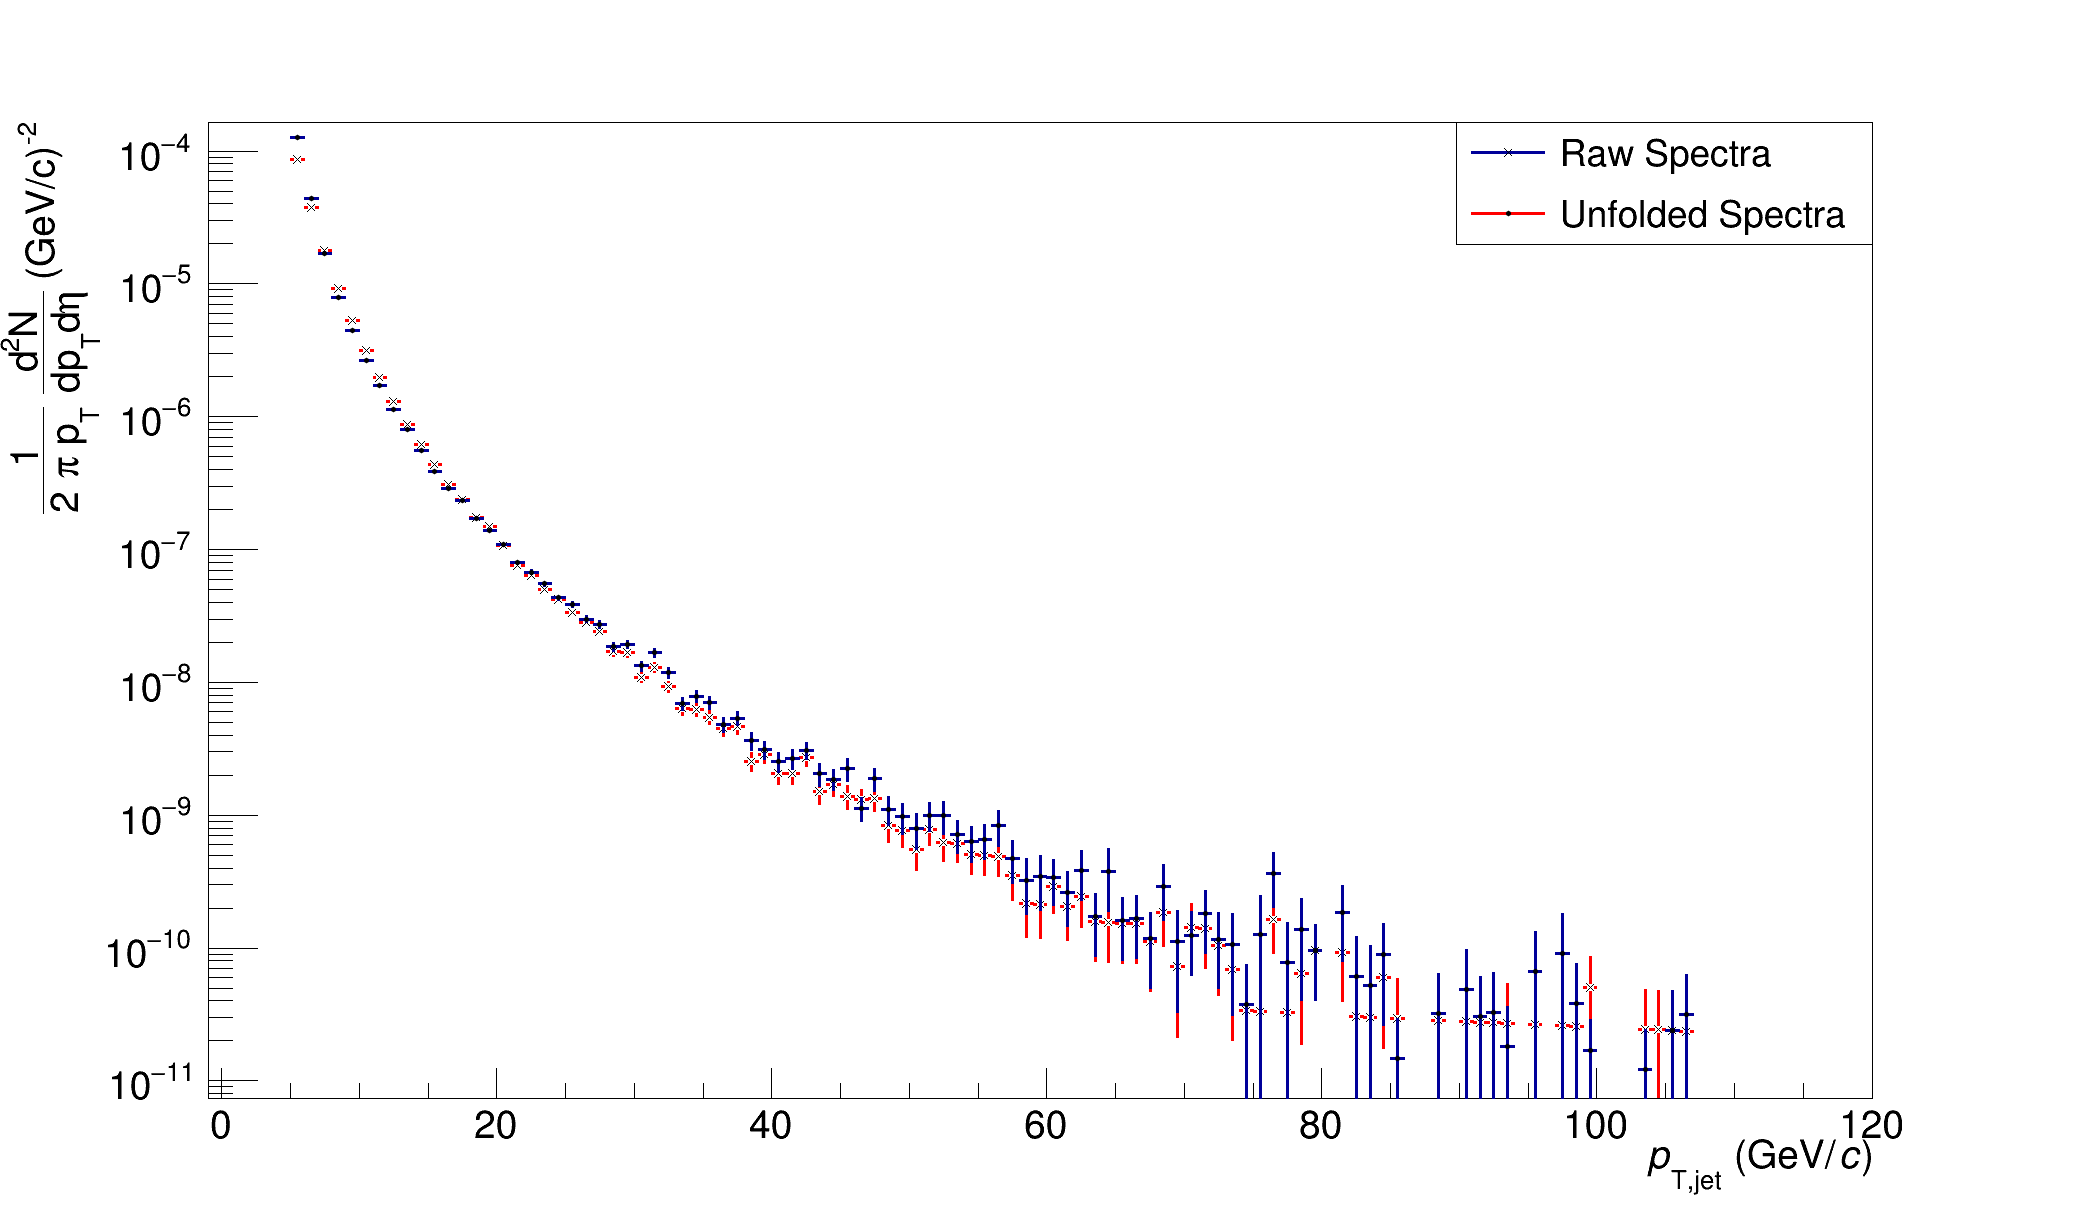
\includegraphics[width=8cm]{RawandUnfoldedSpectraMBR03}
\centering
\caption{Unfolded jet spectra with fine binning for R = 0.3}
\label{fig:Unfoldfine}
\end{figure}

An example of the output from the bin-by-bin unfolding with the fine binning for R = 0.3 jet is shown in Figure \ref{fig:Unfoldfine}.  It should be noted that at low-$p_{T}$ it was observed that unfolding increased the yield of the spectra while at high-$p_{T} \geq \,$ 40 GeV the yield was decreased for all jet radii in this analysis.  This is most likely due to the lack of statistics in the response matrix.  Once the bin-by-bin unfolding has been performed for the fine binned spectra the output along with the bin-by-bin correction factors are rebinned using a variable binning between 10 GeV and 120 GeV, these corrected spectra are shown in Figure \ref{fig:unfoldMinbias}.


\begin{figure*}[t!]
$\begin{array}{rl}
    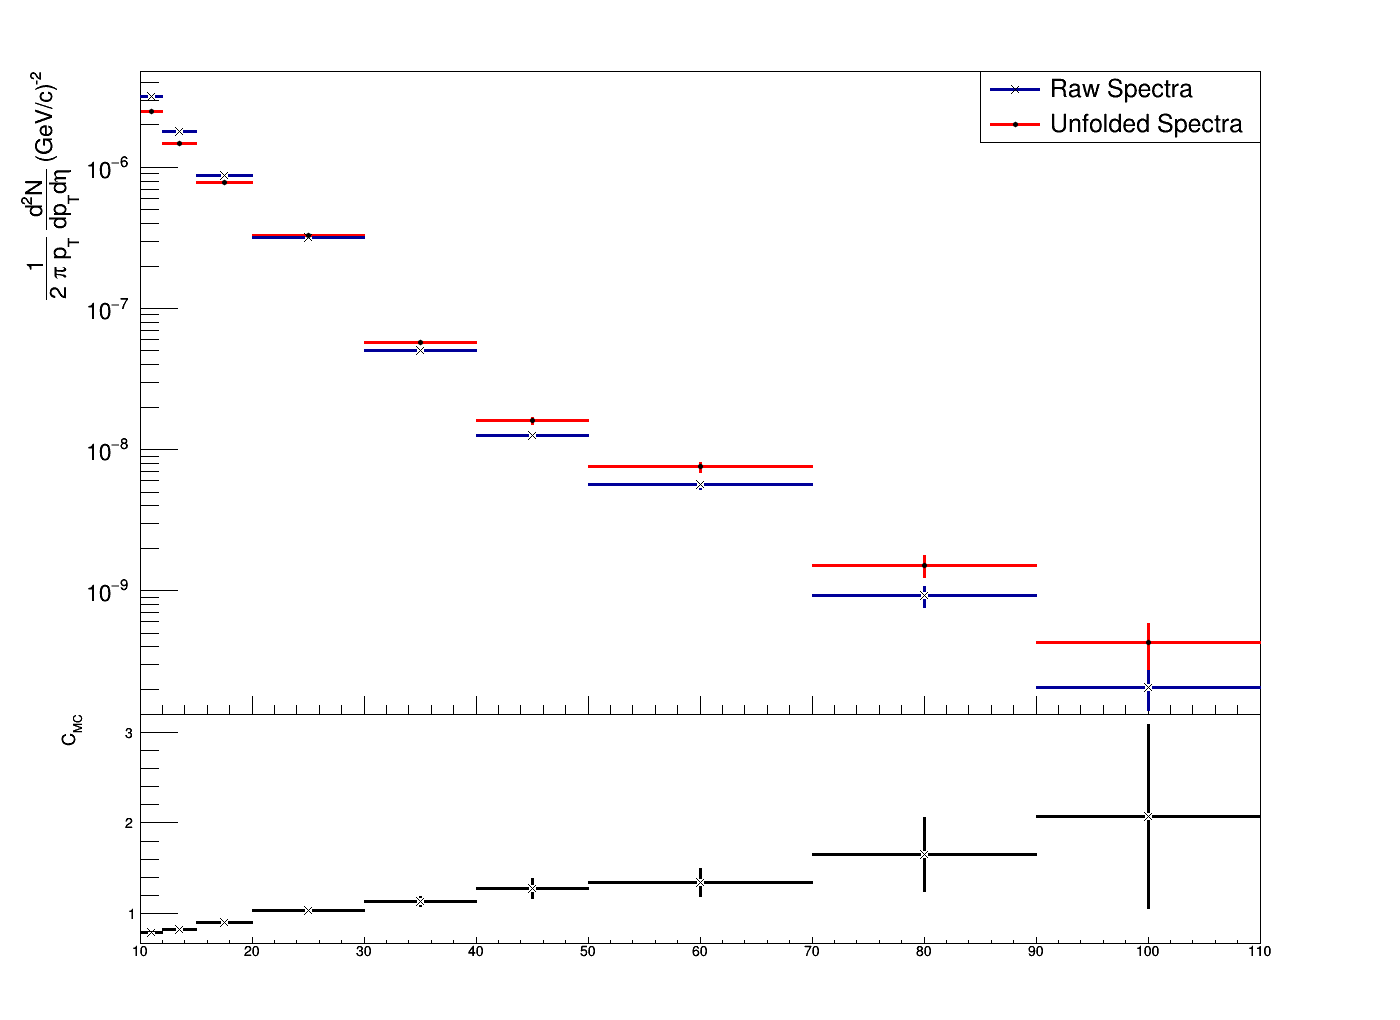
\includegraphics[width=0.5\textwidth]{UnfoldedR02MinBias} &
    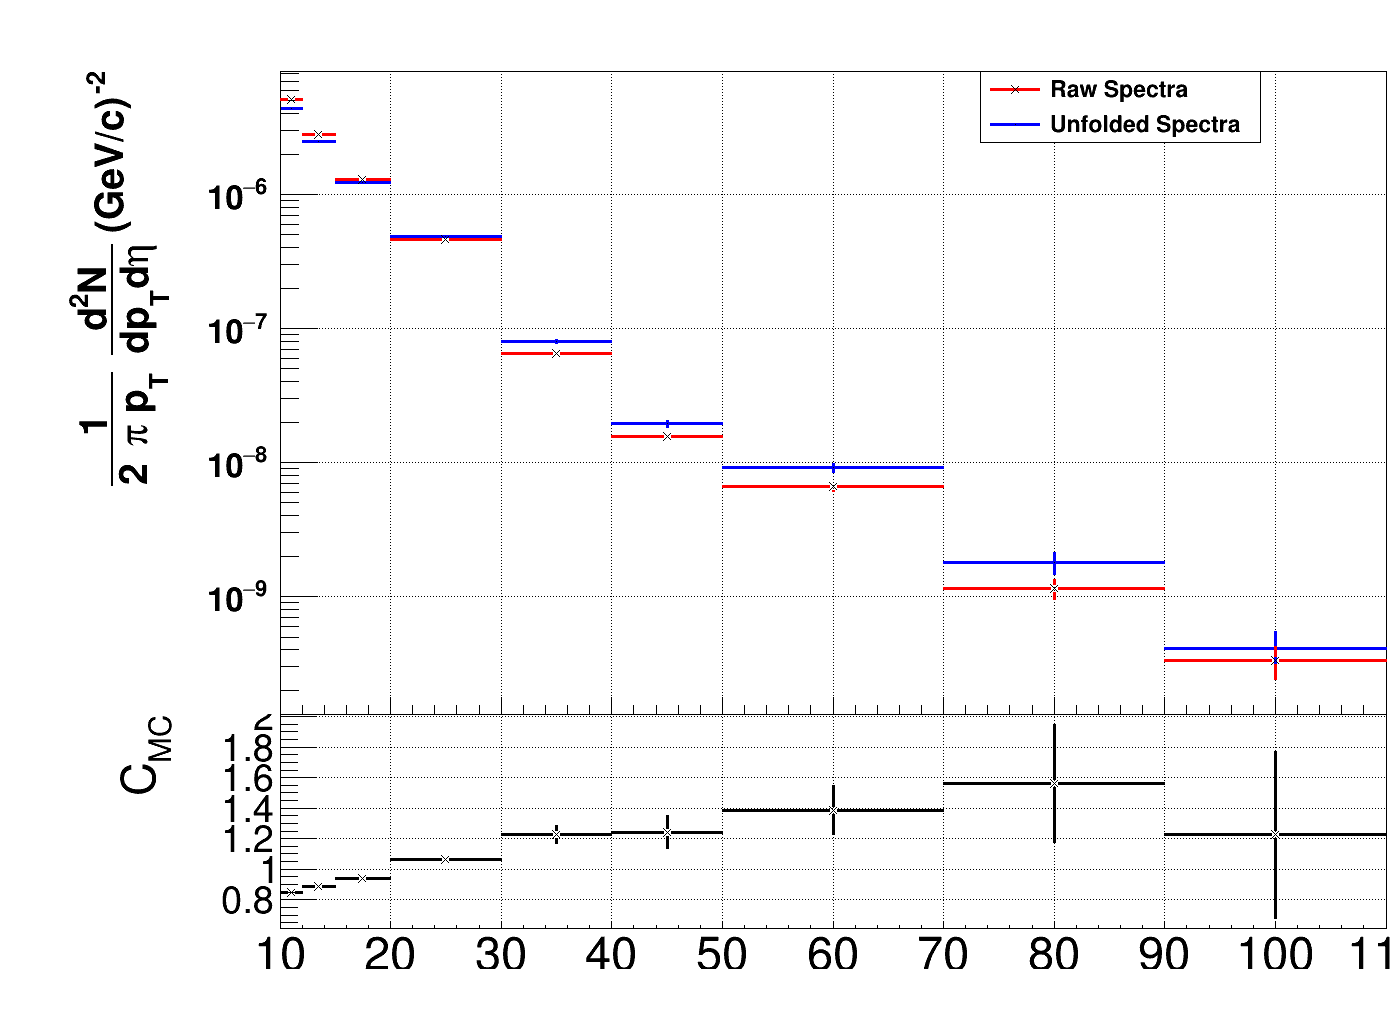
\includegraphics[width=0.5\textwidth]{UnfoldedR03MinBias}\\
    \multicolumn{2}{c}{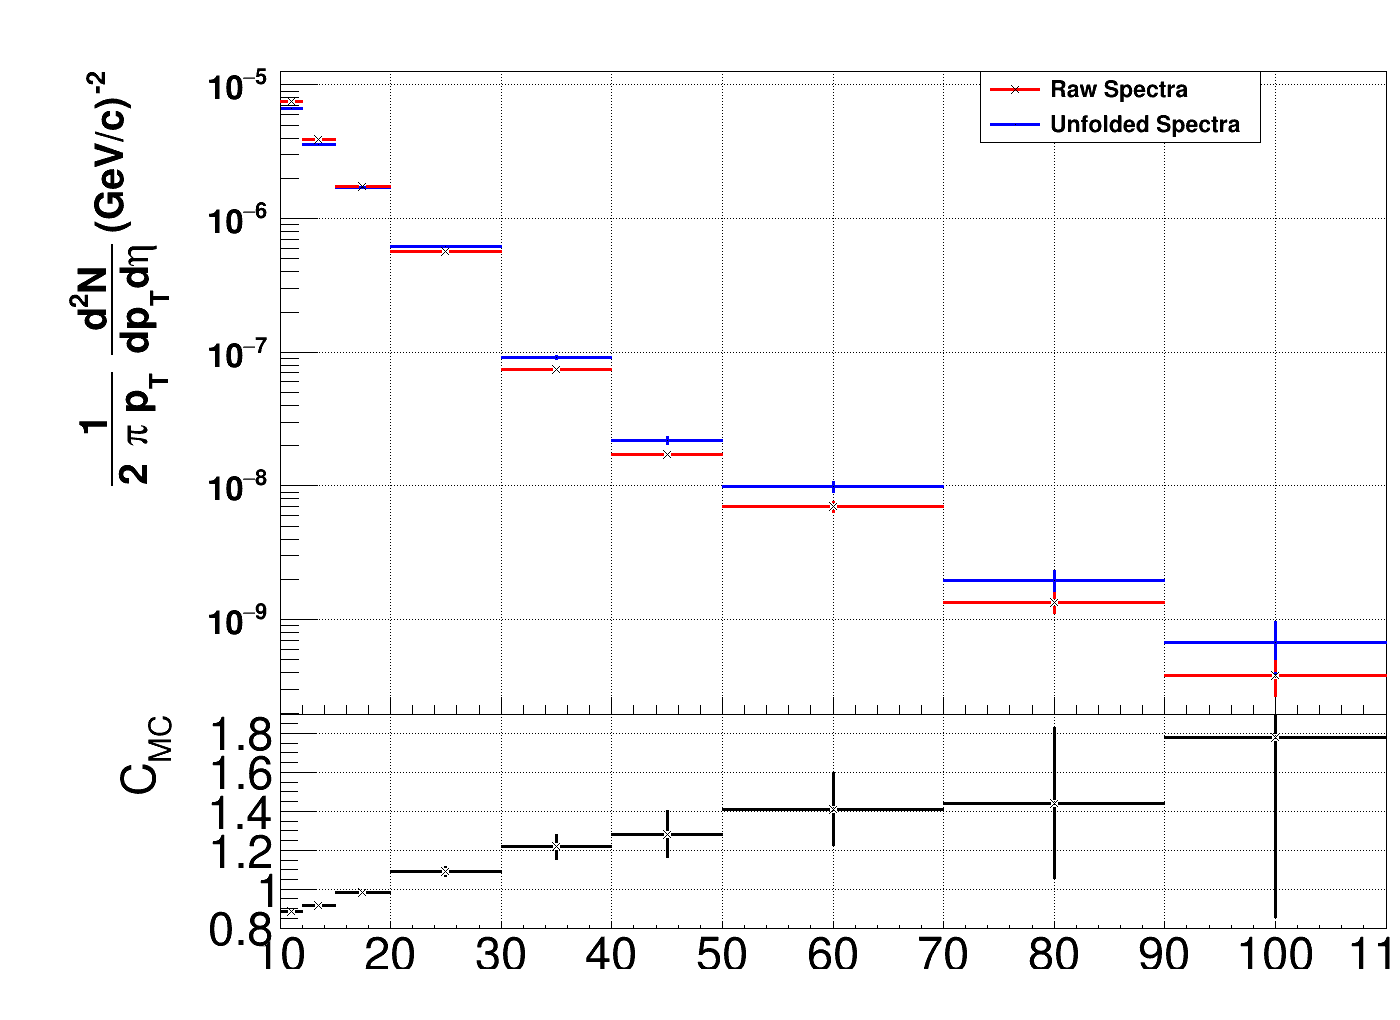
\includegraphics[width=0.5\textwidth]{UnfoldedR04MinBias}}
\end{array}$
\caption[Corrected Jet Spectra to Monte Carlo level for R = 0.2, R=0.3, and R = 0.4 jets.]{\label{fig:unfoldMinbias}Unfolded Min Bias Jet Spectra with correction factors, $C_{MC}$, for R = 0.2, R=0.3, and R = 0.4 jets.}
\end{figure*}

\subsubsection{Unfolded EMCal Triggered Spectra}
The unfolding procedure was repeated again for the EMCal triggered jet spectra.  The response matrix from the Min Bias sample was used for the bin-by-bin unfolding and performed using a fine binning.  The detector level and particle level jets were configured in the same manner as above and the output from the unfolded triggered spectra were reported after rebinning to a variable size over the same kinematic range, as seen in Figure \ref{fig:unfoldEGA}.

\begin{figure*}[t!]
$\begin{array}{rl}
    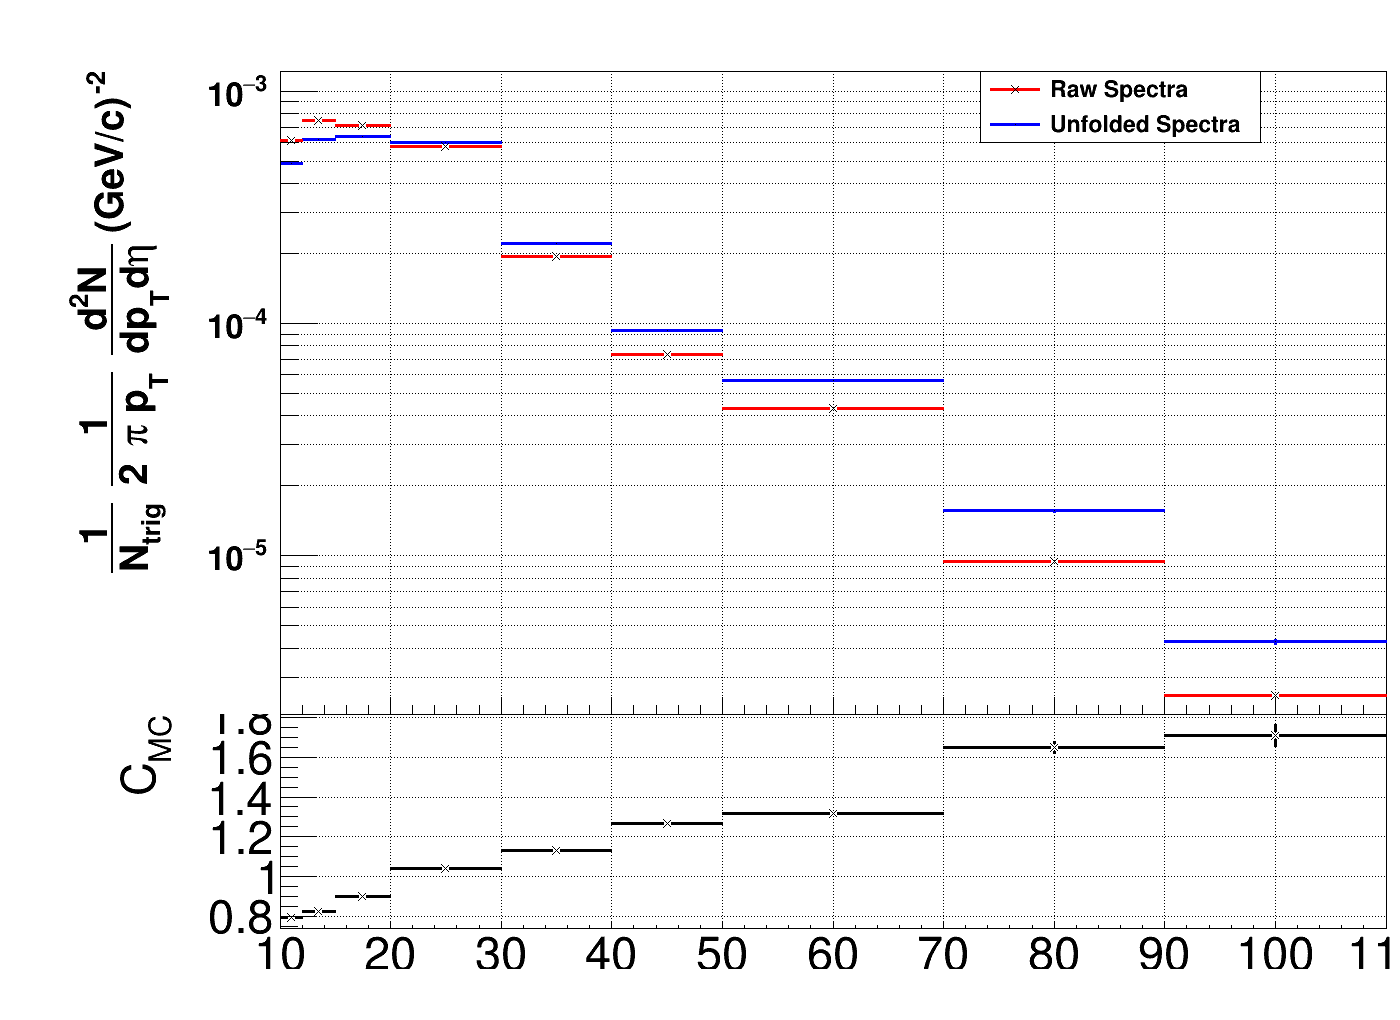
\includegraphics[width=0.5\textwidth]{UnfoldedR02EGAtrigger} &
    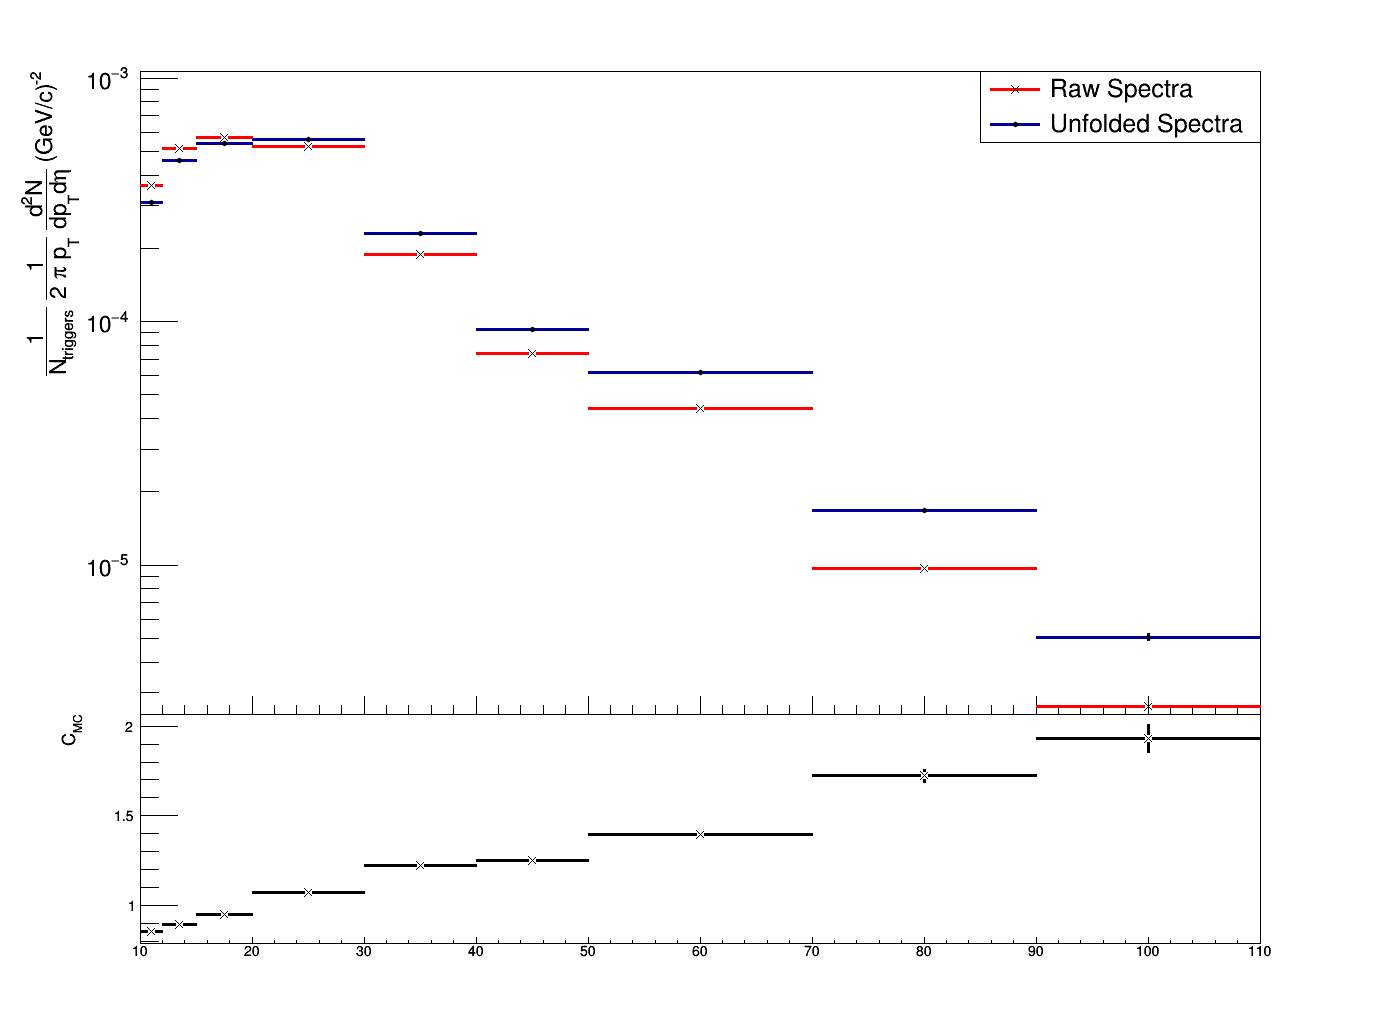
\includegraphics[width=0.5\textwidth]{UnfoldedR03EGAtrigger}\\
    \multicolumn{2}{c}{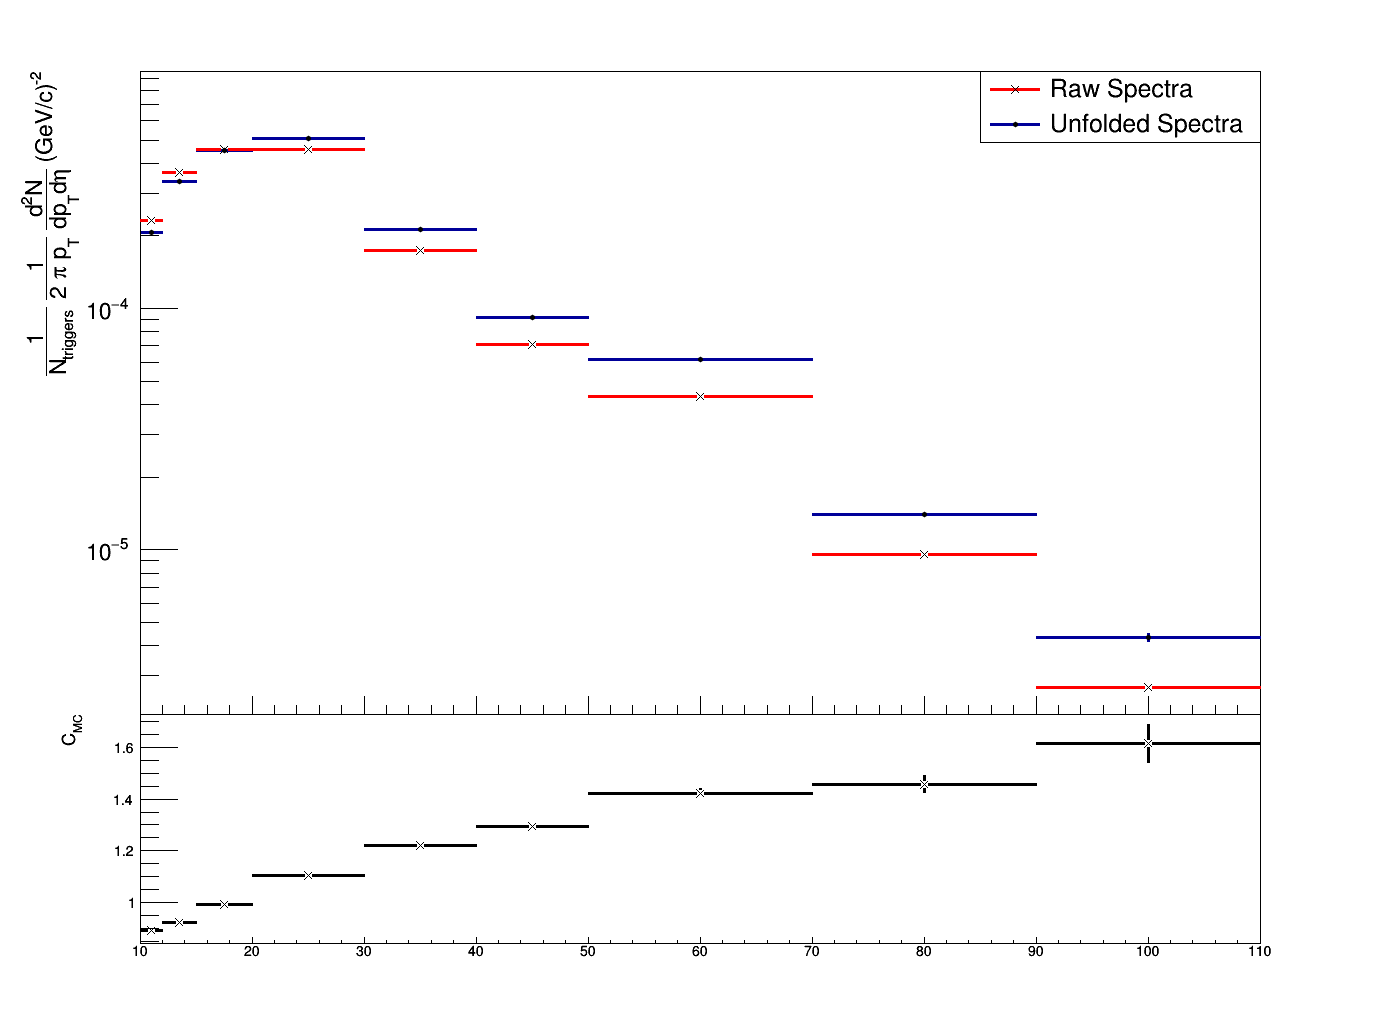
\includegraphics[width=0.5\textwidth]{UnfoldedR04EGAtrigger}}
\end{array}$
\caption[Corrected EMCal Triggered Jet Spectra to Monte Carlo level for R = 0.2, R=0.3, and R = 0.4 jets.]{\label{fig:unfoldEGA}Unfolded EMCal Triggered Jet Spectra with correction factors, $C_{MC}$, for R = 0.2, R=0.3, and R = 0.4 jets.}
\end{figure*}


Due to the limitations of the response matrix, the bin-by-bin unfolding of the EMCal triggered data was only stable up to 120 GeV.  Again, it should be noted that the hump in the EMCal jet spectra is due to the firing threshold of the trigger.  The unfolded EMCal jet spectra was used to estimate the ratio that the jet yields between the Min Bias and triggered data samples, from this point the trigger scaling was calculated.  Due to the lack of a trigger modeled with the 8 TeV Monte Carlo productions, were unable to extend the kinematic range of the jet spectras beyond 120 GeV.  This presents a missed opportunity in terms of the recorded data from the 8 TeV runs.  In order to address this issue a new Monte Carlo production will need to be requested from the ALICE collaboration.

\section{Jet Reconstruction and Matching Efficiency}
In order to quantify the inefficiencies due to unfolding along with the inefficiencies in the ALICE experiment in reconstructing jets, we quantify the jet reconstruction efficiency, $\epsilon_{reco} (p_{T, jet})$, and the jet matching efficiency, $\epsilon_{match} (p_{T, jet})$.

\begin{equation}
 \epsilon_{reco} (p_{T, jet}) = \frac{N_{reco}(p_{T, jet}) }{N_{Truth} (p_{T, jet})}
\label{eq:jetrecoeff}
\end{equation}

\begin{equation}
 \epsilon_{match} (p_{T, jet}) = \frac{N_{match}(p_{T, jet}) }{N_{Truth}(p_{T, jet})}
\label{eq:jetmatchoeff}
\end{equation}

\noindent 
where $N_{reco} (p_{T, jet})$ is the reconstructed jet yield at the detector level per $p_{T}$ bin, $N_{match}(p_{T, jet})$ is the reconstructed jet at the detector level that was matched to a particle level jet per $p_{T}$ bin, and $N_{truth} (p_{T, jet})$ is the truth-level particle jet yield from the Pythia embedded event per $p_{T}$ bin.  

The $N_{truth} (p_{T, jet})$ were obtained by running FastJet on Pythia events with no constituent $p_{T}$ cut, while $N_{match}(p_{T, jet})$ and $N_{reco} (p_{T, jet})$ had the same kinematic cuts as the data driven analysis mentioned earlier in this chapter.  The truth level jets contained no geometric acceptance cut in order to account for jets that may have been reconstructed at the detector level, but had no match to a particle level because part of the particle level jet was outside the EMCal acceptance.  The spectrums were corrected by these efficiencies after the bin-by-bin corrections were performed.  The correction factors are shown in Figures \ref{fig:JetMatcheff} and \ref{fig:JetRecoeff}.

\begin{figure*}[t!]
$\begin{array}{rl}
    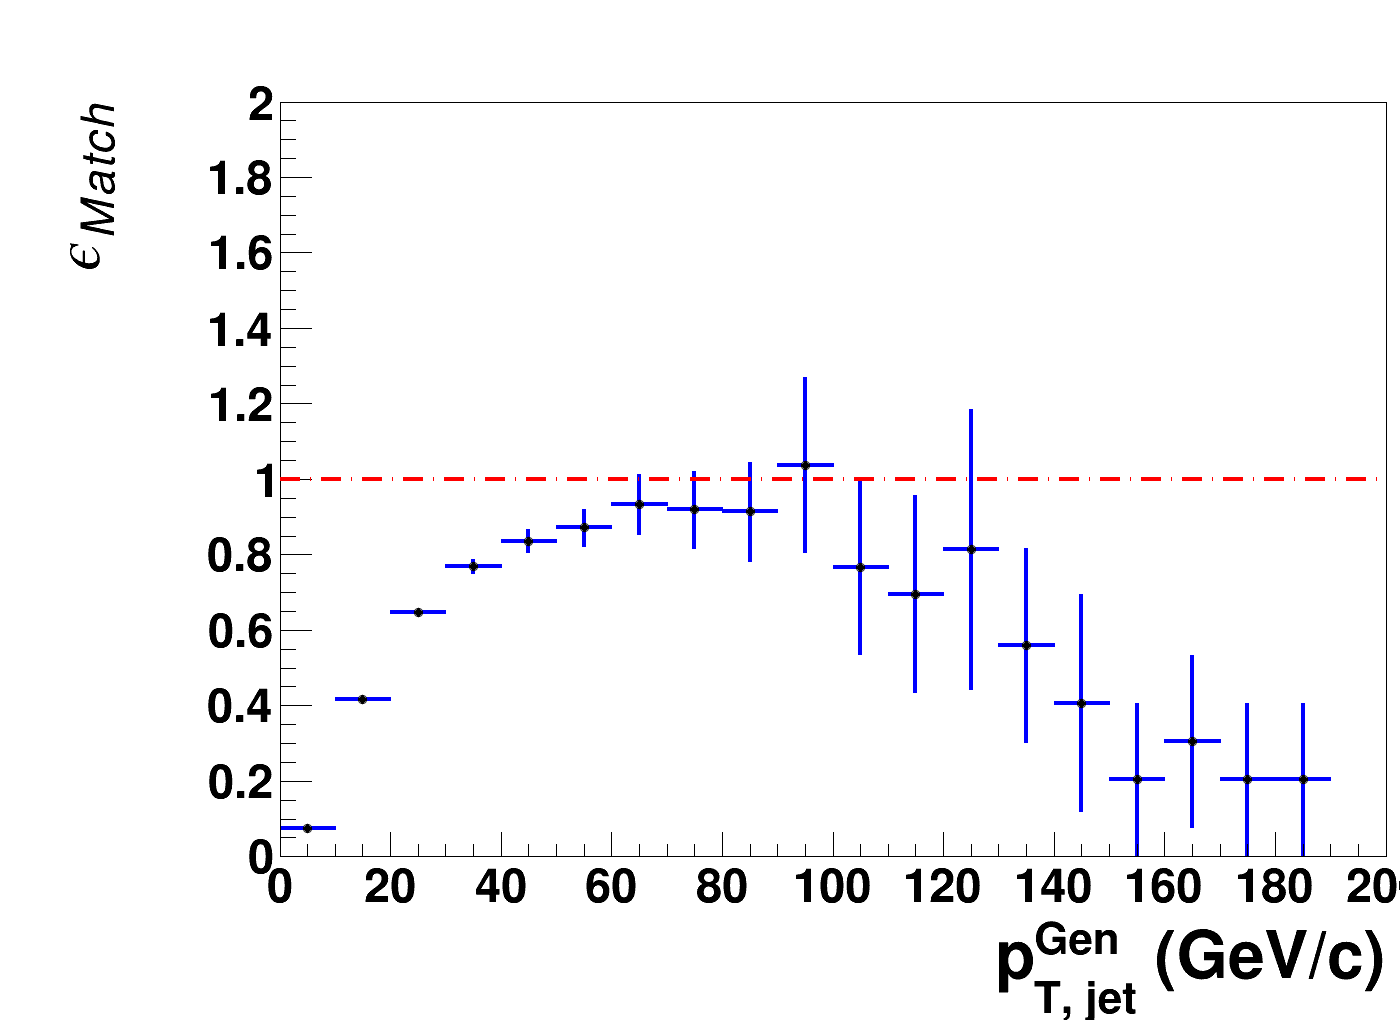
\includegraphics[width=0.5\textwidth]{Ematch_R02} &
    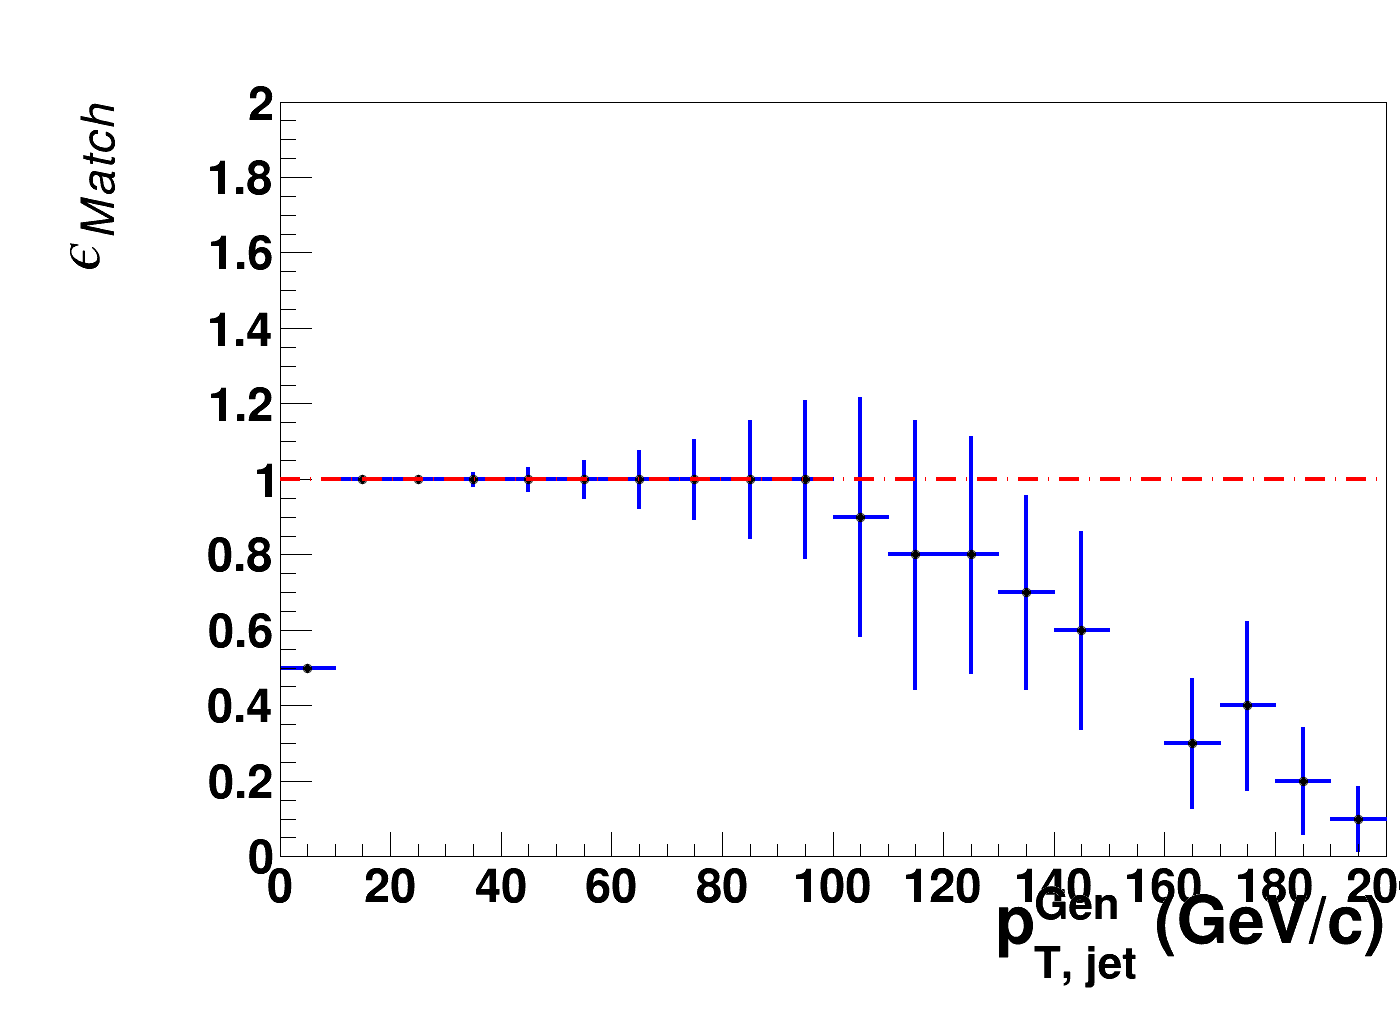
\includegraphics[width=0.5\textwidth]{Ematch_R03}\\
    \multicolumn{2}{c}{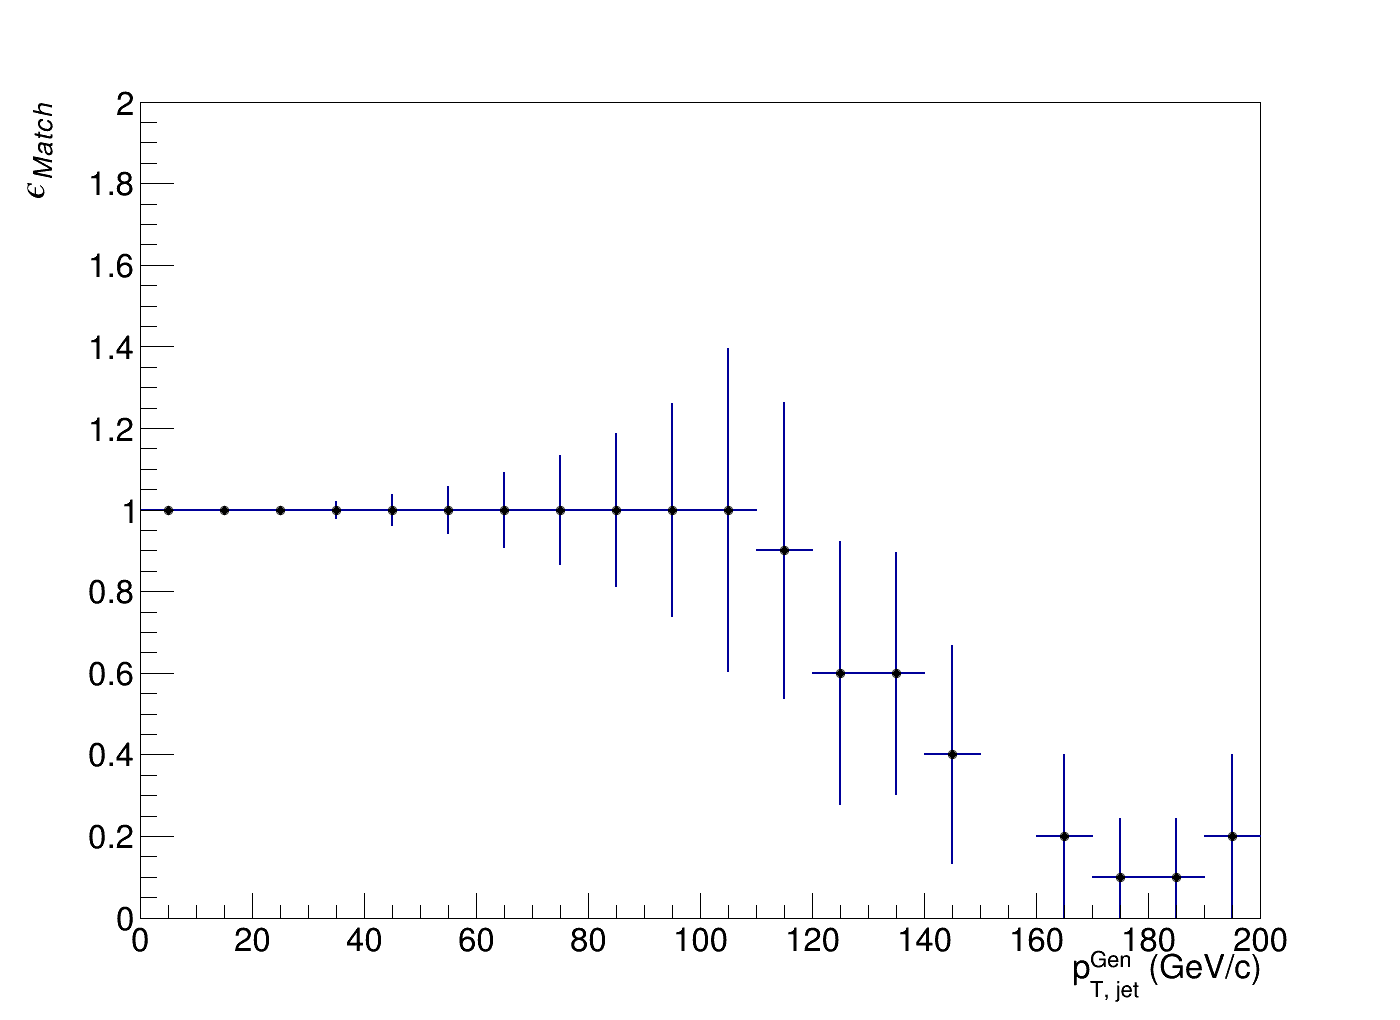
\includegraphics[width=0.5\textwidth]{Ematch_R04}}
\end{array}$
\caption[Jet reconstruction efficiency for jets between R = 0.2 and R = 0.4. ]{\label{fig:JetMatcheff}Jet matching efficiency for jets between R = 0.2 and R = 0.4.}
\end{figure*}

\begin{figure*}[t!]
$\begin{array}{rl}
    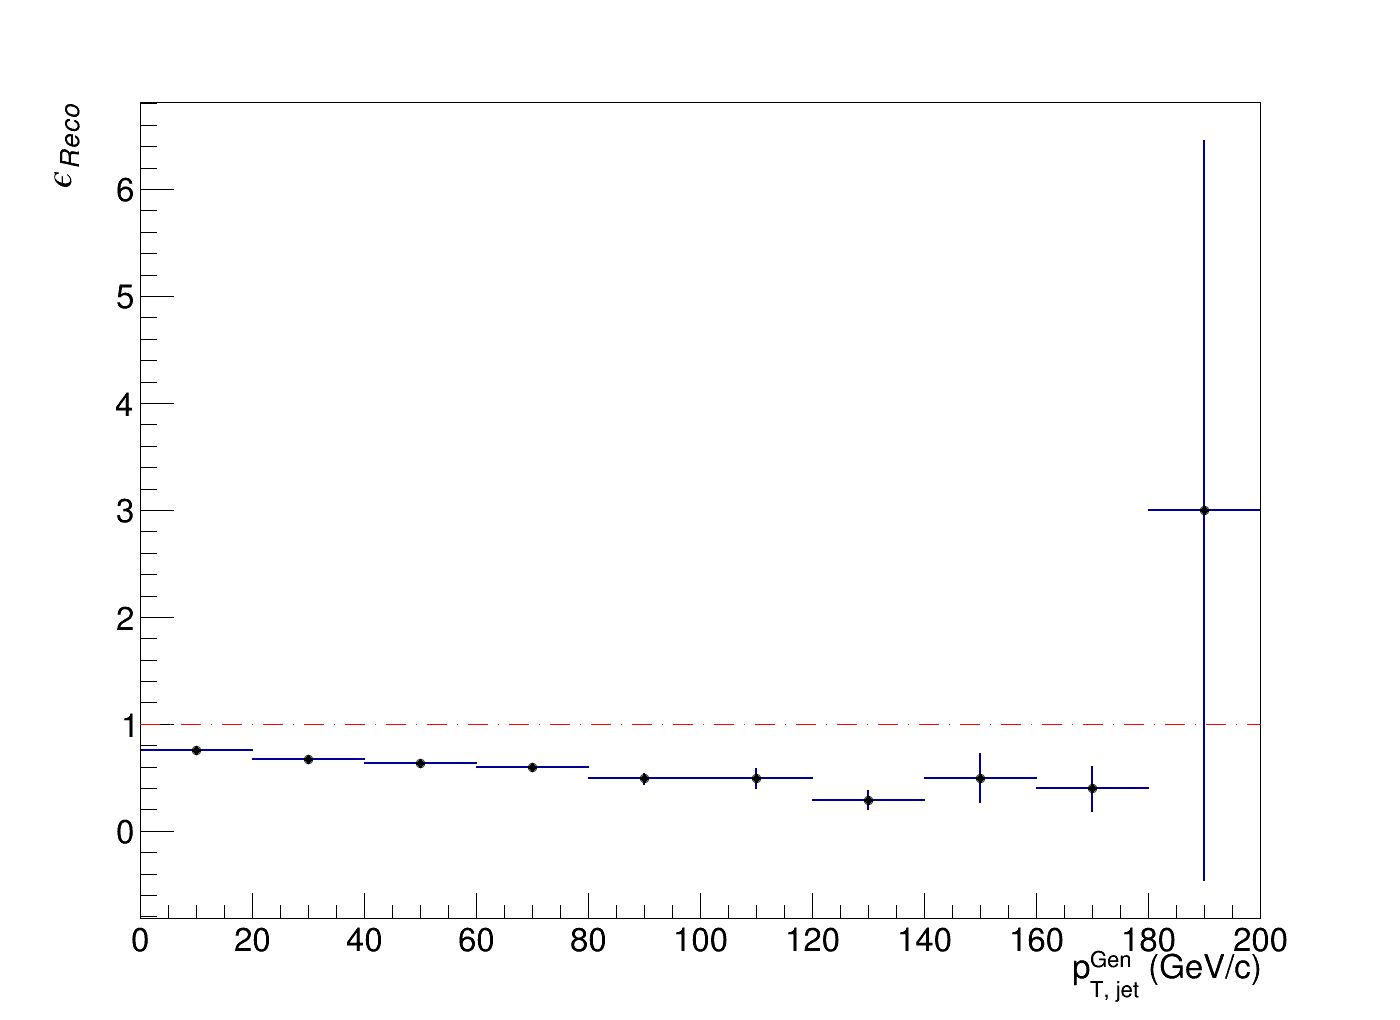
\includegraphics[width=0.5\textwidth]{Ereco_R02} &
    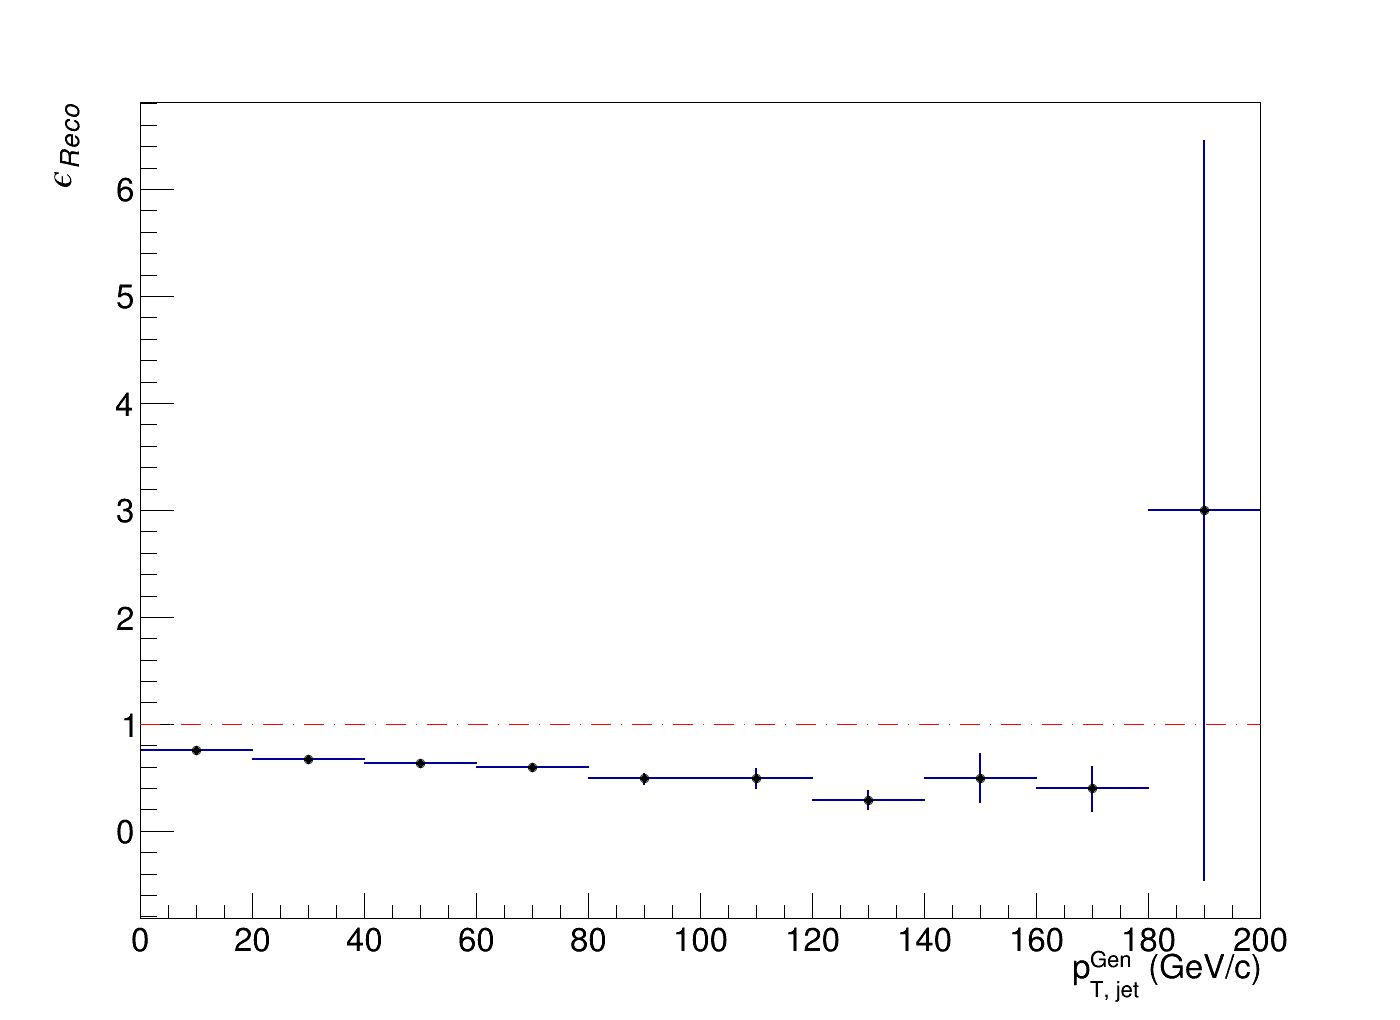
\includegraphics[width=0.5\textwidth]{Ereco_R02}\\
    \multicolumn{2}{c}{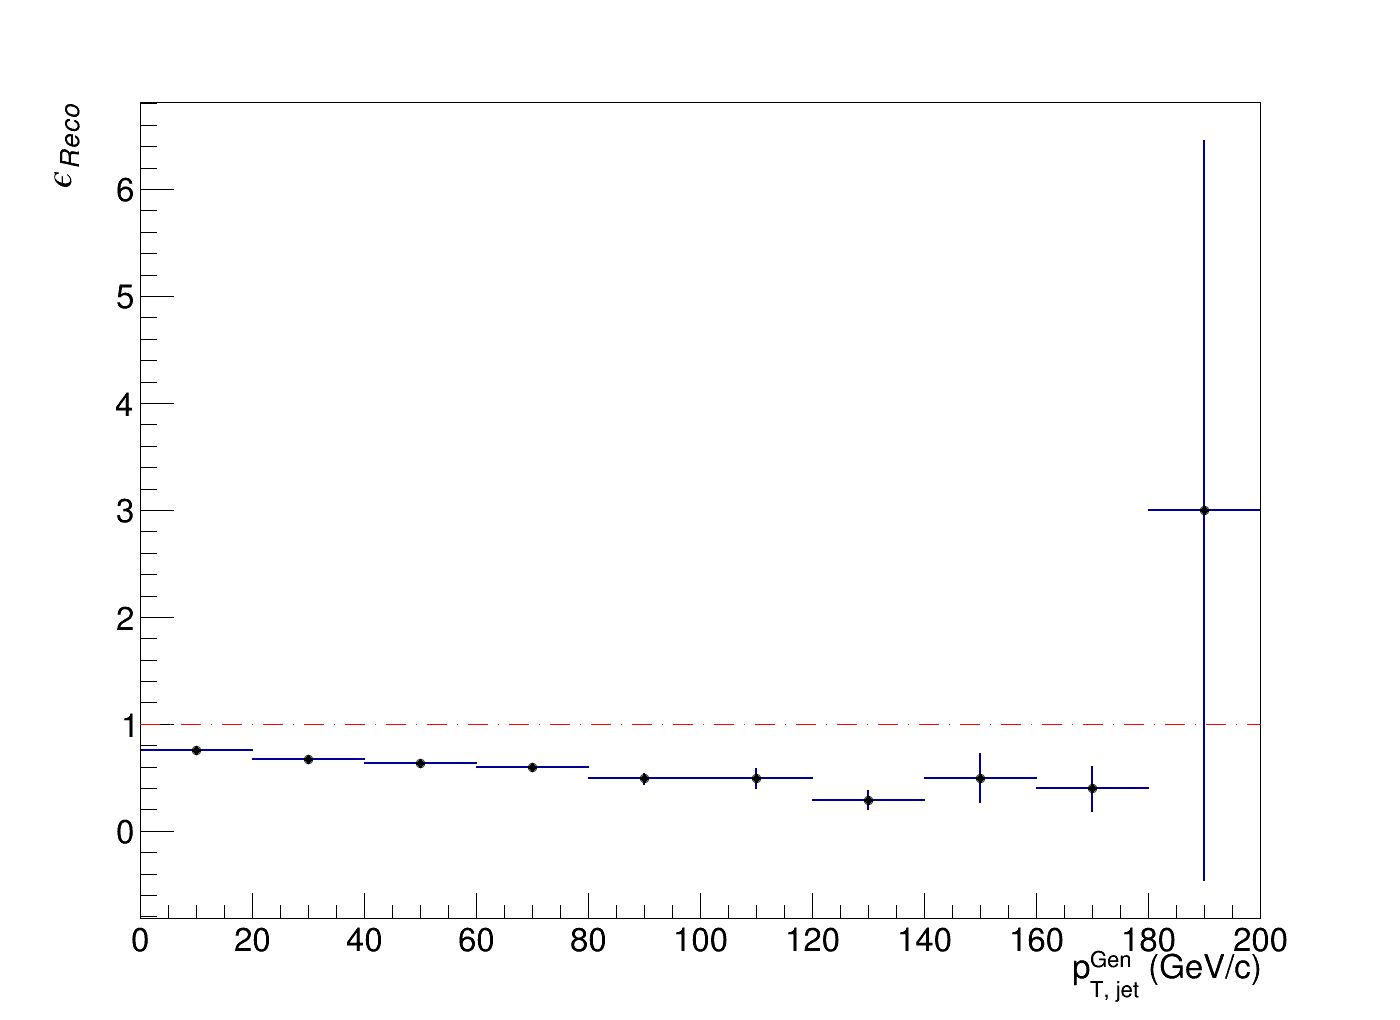
\includegraphics[width=0.5\textwidth]{Ereco_R02}}
\end{array}$
\caption[Jet reconstruction efficiency for jets between R = 0.2 and R = 0.4.]{\label{fig:JetRecoeff}Jet reconstruction efficiency for jets between R = 0.2 and R = 0.4}
\end{figure*}


The major steps performed for this thesis have been described in this chapter.  The final chapter will go over the systematic errors reported for the final results, present the final cross-sections measured at 8 TeV, and compare these results to previous measurements and  calculations.

